\section{eplustbl.\textless{}ext\textgreater{}}\label{eplustbl.ext}

The eplustbl file contains the tabular output results that are created when using the following objects:

\begin{itemize}
\item
  Output:Table:SummaryReports
\item
  Output:Table:TimeBins
\item
  Output:Table:Monthly
\item
  UtilityCost:Tariff
\item
  ComponentCost:Line Item
\end{itemize}

The format and the extension for the file depends on the setting of the ColumnSeparator field of the Output:Table:Style object. The choices of HTML, tab, fixed, comma, and XML result in eplustbl.htm, eplustbl.tab, eplustbl.txt, eplustbl.csv, eplustbl.xml respectively. The HTML version of the report also includes a table of contents that allows easier navigation through the file.

By default the energy units reported in all of the eplustbl files are in Joules (J) but the UnitConversion field of the Output:Table:Style object allows for the values to be reported in MJ, GJ or in kWh. In addition, the Output:Table:Style object can specify for the tables to be in IP units for all fields.

\subsection{Output:Table:SummaryReports}\label{outputtablesummaryreports}

Several predefined reports are available from the Output:Table:SummaryReports object including the following. (spaces are inserted in names for readability; keys are included in the Input Data Dictionary or by just removing the spaces):

\begin{itemize}
\tightlist
\item
  All Summary
\end{itemize}

Lists all following applicable tables with ``Summary'' in the name.

\begin{itemize}
\tightlist
\item
  All Monthly
\end{itemize}

Lists all following applicable tables with ``Monthly'' in the name.

\begin{itemize}
\tightlist
\item
  All Summary And Monthly
\end{itemize}

Lists all following applicable tables with both ``Summary'' and ``Monthly'' in the name. This does not include the Zone Component Load Summary report.

\begin{itemize}
\tightlist
\item
  All Summary and Sizing Period
\end{itemize}

Lists the All Summary tables as well as the Zone Component Load report (currently the only Sizing Period report). Please note that the Zone Component Load report does increase the run time because it repeats sizing periods.

\begin{itemize}
\tightlist
\item
  All Summary Monthly and Sizing Period
\end{itemize}

Lists the All Summary tables, the Monthly tables as well as the Zone Component Load report (currently the only Sizing Period report). Please note that the Zone Component Load report does increase the run time because it repeats sizing periods.

\begin{itemize}
\item
  Annual Building Utility Performance Summary
\item
  Input Verification and Results Summary
\item
  Demand End Use Components Summary
\item
  Source Energy End Use Components Summary
\item
  Climatic Data Summary
\item
  Equipment Summary
\item
  Envelope Summary
\item
  Surface Shadowing Summary
\item
  Shading Summary
\item
  Lighting Summary
\item
  HVAC Sizing Summary
\item
  System Summary
\item
  HVAC Topology
\item
  Component Sizing Summary
\item
  Outdoor Air Summary
\item
  Outdoor Air Details
\item
  Object Count Summary
\item
  Component Cost Economics Summary
\item
  Energy Meters
\item
  Sensible Heat Gain Summary
\item
  Standard 62.1 Summary
\item
  Zone Component Load Summary
\item
  Zone Cooling Summary Monthly
\item
  Zone Heating Summary Monthly
\item
  Zone Electric Summary Monthly
\item
  Space Gains Monthly
\item
  Peak Space Gains Monthly
\item
  Space Gain Components At Cooling Peak Monthly
\item
  Energy Consumption Electricity Natural Gas Monthly
\item
  Energy Consumption Electricity Generated Propane Monthly
\item
  Energy Consumption Diesel FuelOil Monthly
\item
  Energy Consumption District Heating Cooling Monthly
\item
  Energy Consumption Coal Gasoline Monthly
\item
  End Use Energy Consumption Electricity Monthly
\item
  End Use Energy Consumption NaturalGas Monthly
\item
  End Use Energy Consumption Diesel Monthly
\item
  End Use Energy Consumption FuelOil Monthly
\item
  End Use Energy Consumption Coal Monthly
\item
  End Use Energy Consumption Propane Monthly
\item
  End Use Energy Consumption Gasoline Monthly
\item
  Peak Energy End Use Electricity Part1 Monthly
\item
  Peak Energy End Use Electricity Part2 Monthly
\item
  Electric Components Of Peak Demand Monthly
\item
  Peak Energy End Use NaturalGas Monthly
\item
  Peak Energy End Use Diesel Monthly
\item
  Peak Energy End Use FuelOil Monthly
\item
  Peak Energy End Use Coal Monthly
\item
  Peak Energy End Use Propane Monthly
\item
  Peak Energy End Use Gasoline Monthly
\item
  Setpoints Not Met With Temperatures Monthly
\item
  Comfort Report Simple55 Monthly
\item
  Unglazed Transpired Solar Collector Summary Monthly
\item
  Occupant Comfort Data Summary Monthly
\item
  Chiller Report Monthly
\item
  Tower Report Monthly
\item
  Boiler Report Monthly
\item
  DX Report Monthly
\item
  Window Report Monthly
\item
  Window Energy Report Monthly
\item
  Window Zone Summary Monthly
\item
  Window Energy Zone Summary Monthly
\item
  Average Outdoor Conditions Monthly
\item
  Outdoor Conditions Maximum DryBulb Monthly
\item
  Outdoor Conditions Minimum DryBulb Monthly
\item
  Outdoor Conditions Maximum WetBulb Monthly
\item
  Outdoor Conditions Maximum DewPoint Monthly
\item
  Outdoor Ground Conditions Monthly
\item
  WindowAC Report Monthly
\item
  Water Heater Report Monthly
\item
  Generator Report Monthly
\item
  Daylighting Report Monthly
\item
  Coil Report Monthly
\item
  PlantLoop Demand Report Monthly
\item
  Fan Report Monthly
\item
  Pump Report Monthly
\item
  CondLoop Demand Report Monthly
\item
  Zone Temperature Oscillation Report Monthly
\item
  AirLoop System Energy And Water Use Monthly
\item
  AirLoop System Component Loads Monthly
\item
  AirLoop System Component Energy Use Monthly
\item
  Mechanical Ventilation Loads Monthly
\end{itemize}

Each of these reports is made up of several sub-tables of information. Examples of some of the tables are shown below. To enable all of the reports the single All Summary may be specified.

\subsection{Annual Building Utility Performance Summary}\label{annual-building-utility-performance-summary}

The Annual Building Utility Performance Summary report provides an overview of energy consumption in the building for different end uses. The following is an example this report (some columns may be truncated due to page size). The key used to obtain this report is AnnualBuildingUtilityPerformanceSummary.

In the \emph{Comfort and Setpoint Not Met Summary} sub-table, facility hours represents the total number of hours that any single zone did not meet the comfort or setpoint criteria. It is not weighted by number of zones or number of occupants.

The values in the \emph{End Uses} sub-table are from report meters. To determine which components are attached to each end-use meter, consult the meter details output file (*.mtd).

Report: Annual Building Utility Performance Summary

For: Entire Facility

Timestamp: 2009-02-10 12:39:35

Values gathered over 8760.00 hours

Site and Source Energy

\begin{longtable}[c]{>{\raggedright}p{1.5in}>{\raggedright}p{1.5in}>{\raggedright}p{1.5in}>{\raggedright}p{1.5in}}
\toprule 
~ & Total Energy (GJ) & Energy Per Total Building Area (MJ/m2) & Energy Per Conditioned Building Area (MJ/m2) \tabularnewline
\midrule
\endfirsthead

\toprule 
~ & Total Energy (GJ) & Energy Per Total Building Area (MJ/m2) & Energy Per Conditioned Building Area (MJ/m2) \tabularnewline
\midrule
\endhead

Total Site Energy & 194.80 & 210.09 & 210.09 \tabularnewline
Net Site Energy & 194.80 & 210.09 & 210.09 \tabularnewline
Total Source Energy & 532.25 & 574.04 & 574.04 \tabularnewline
Net Source Energy & 532.25 & 574.04 & 574.04 \tabularnewline
\bottomrule
\end{longtable}

Source to Site Energy Converstion Factors

\begin{longtable}[c]{@{}ll@{}}
\toprule 
~ & Source= > Site Conversion Factor \tabularnewline
\midrule
\endfirsthead

\toprule 
~ & Source= > Site Conversion Factor \tabularnewline
\midrule
\endhead

Electricity & 3.167 \tabularnewline
Natural Gas & 1.084 \tabularnewline
District Cooling & 1.056 \tabularnewline
District Heating & 3.613 \tabularnewline
Steam & 0.300 \tabularnewline
Gasoline & 1.050 \tabularnewline
Diesel & 1.050 \tabularnewline
Coal & 1.050 \tabularnewline
Fuel Oil No 1 & 1.050 \tabularnewline
Fuel Oil No 2 & 1050 \tabularnewline
Propane & 1.050 \tabularnewline
\bottomrule
\end{longtable}

Building Area

\begin{longtable}[c]{@{}ll@{}}
\toprule 
~ & Area (m2) \tabularnewline
\midrule
\endfirsthead

\toprule 
~ & Area (m2) \tabularnewline
\midrule
\endhead

Total Building Area & 927.20 \tabularnewline
Net Conditioned Building Area & 927.20 \tabularnewline
Unconditioned Building Area & 0.00 \tabularnewline
\bottomrule
\end{longtable}

End Uses

{\scriptsize
\begin{longtable}[c]{>{\raggedright}p{0.85in}>{\raggedright}p{0.85in}>{\raggedright}p{0.85in}>{\raggedright}p{0.85in}>{\raggedright}p{0.85in}>{\raggedright}p{0.85in}>{\raggedright}p{0.85in}}
\toprule 
~ & Electricity (GJ) & Natural Gas (GJ) & Other Fuel (GJ) & District Cooling (GJ) & District Heating (GJ) & Water (m3) \tabularnewline
\midrule
\endfirsthead

\toprule 
~ & Electricity (GJ) & Natural Gas (GJ) & Other Fuel (GJ) & District Cooling (GJ) & District Heating (GJ) & Water (m3) \tabularnewline
\midrule
\endhead

Heating & 0.00 & 40.65 & 0.00 & 0.00 & 0.00 & 0.00 \tabularnewline
Cooling & 18.18 & 0.00 & 0.00 & 0.00 & 0.00 & 0.00 \tabularnewline
Interior Lighting & 81.24 & 0.00 & 0.00 & 0.00 & 0.00 & 0.00 \tabularnewline
Exterior Lighting & 0.00 & 0.00 & 0.00 & 0.00 & 0.00 & 0.00 \tabularnewline
Interior Equipment & 47.70 & 0.00 & 0.00 & 0.00 & 0.00 & 0.00 \tabularnewline
Exterior Equipment & 0.00 & 0.00 & 0.00 & 0.00 & 0.00 & 0.00 \tabularnewline
Fans & 7.03 & 0.00 & 0.00 & 0.00 & 0.00 & 0.00 \tabularnewline
Pumps & 0.00 & 0.00 & 0.00 & 0.00 & 0.00 & 0.00 \tabularnewline
Heat Rejection & 0.00 & 0.00 & 0.00 & 0.00 & 0.00 & 0.00 \tabularnewline
Humidification & 0.00 & 0.00 & 0.00 & 0.00 & 0.00 & 0.00 \tabularnewline
Heat Recovery & 0.00 & 0.00 & 0.00 & 0.00 & 0.00 & 0.00 \tabularnewline
Water Systems & 0.00 & 0.00 & 0.00 & 0.00 & 0.00 & 0.00 \tabularnewline
Refrigeration & 0.00 & 0.00 & 0.00 & 0.00 & 0.00 & 0.00 \tabularnewline
Generators & 0.00 & 0.00 & 0.00 & 0.00 & 0.00 & 0.00 \tabularnewline
~ & ~ & ~ & ~ & ~ & ~ & ~ \tabularnewline
Total End Uses & 154.15 & 40.65 & 0.00 & 0.00 & 0.00 & 0.00 \tabularnewline
\bottomrule
\end{longtable}}

\emph{Note: Natural gas appears to be the principal heating source based on energy usage.}

End Uses By Subcategory

{\scriptsize
\begin{longtable}[c]{>{\raggedright}p{0.75in}>{\raggedright}p{0.75in}>{\raggedright}p{0.75in}>{\raggedright}p{0.75in}>{\raggedright}p{0.75in}>{\raggedright}p{0.75in}>{\raggedright}p{0.75in}>{\raggedright}p{0.75in}}
\toprule 
~ & Subcategory & Electricity (GJ) & Natural Gas (GJ) & Other Fuel (GJ) & District Cooling (GJ) & District Heating (GJ) & Water (m3) \tabularnewline
\midrule
\endfirsthead

\toprule 
~ & Subcategory & Electricity (GJ) & Natural Gas (GJ) & Other Fuel (GJ) & District Cooling (GJ) & District Heating (GJ) & Water (m3) \tabularnewline
\midrule
\endhead

Heating & General & 0.00 & 40.65 & 0.00 & 0.00 & 0.00 & 0.00 \tabularnewline
Cooling & General & 18.18 & 0.00 & 0.00 & 0.00 & 0.00 & 0.00 \tabularnewline
Interior Lighting & GeneralLights & 81.24 & 0.00 & 0.00 & 0.00 & 0.00 & 0.00 \tabularnewline
Exterior Lighting & General & 0.00 & 0.00 & 0.00 & 0.00 & 0.00 & 0.00 \tabularnewline
Interior Equipment & General & 47.70 & 0.00 & 0.00 & 0.00 & 0.00 & 0.00 \tabularnewline
Exterior Equipment & General & 0.00 & 0.00 & 0.00 & 0.00 & 0.00 & 0.00 \tabularnewline
Fans & General & 7.03 & 0.00 & 0.00 & 0.00 & 0.00 & 0.00 \tabularnewline
Pumps & General & 0.00 & 0.00 & 0.00 & 0.00 & 0.00 & 0.00 \tabularnewline
Heat Rejection & General & 0.00 & 0.00 & 0.00 & 0.00 & 0.00 & 0.00 \tabularnewline
Humidification & General & 0.00 & 0.00 & 0.00 & 0.00 & 0.00 & 0.00 \tabularnewline
Heat Recovery & General & 0.00 & 0.00 & 0.00 & 0.00 & 0.00 & 0.00 \tabularnewline
Water Systems & General & 0.00 & 0.00 & 0.00 & 0.00 & 0.00 & 0.00 \tabularnewline
Refrigeration & General & 0.00 & 0.00 & 0.00 & 0.00 & 0.00 & 0.00 \tabularnewline
Generators & General & 0.00 & 0.00 & 0.00 & 0.00 & 0.00 & 0.00 \tabularnewline
\bottomrule
\end{longtable}}

Normalized Metrics

Utility Use Per Conditioned Floor Area

\begin{longtable}[c]{>{\raggedright}p{0.85in}>{\raggedright}p{0.85in}>{\raggedright}p{0.85in}>{\raggedright}p{0.85in}>{\raggedright}p{0.85in}>{\raggedright}p{0.85in}>{\raggedright}p{0.85in}}
\toprule 
~ & Electricity Intensity (MJ/m2) & Natural Gas Intensity (MJ/m2) & Other Fuel Intensity (MJ/m2) & District Cooling Intensity (MJ/m2) & District Heating Intensity (MJ/m2) & Water Intensity (m3/m2) \tabularnewline
\midrule
\endfirsthead

\toprule 
~ & Electricity Intensity (MJ/m2) & Natural Gas Intensity (MJ/m2) & Other Fuel Intensity (MJ/m2) & District Cooling Intensity (MJ/m2) & District Heating Intensity (MJ/m2) & Water Intensity (m3/m2) \tabularnewline
\midrule
\endhead

Lighting & 87.62 & 0.00 & 0.00 & 0.00 & 0.00 & 0.00 \tabularnewline
HVAC & 27.19 & 43.84 & 0.00 & 0.00 & 0.00 & 0.00 \tabularnewline
Other & 51.44 & 0.00 & 0.00 & 0.00 & 0.00 & 0.00 \tabularnewline
Total & 166.25 & 43.84 & 0.00 & 0.00 & 0.00 & 0.00 \tabularnewline
\bottomrule
\end{longtable}

Utility Use Per Total Floor Area

\begin{longtable}[c]{>{\raggedright}p{0.85in}>{\raggedright}p{0.85in}>{\raggedright}p{0.85in}>{\raggedright}p{0.85in}>{\raggedright}p{0.85in}>{\raggedright}p{0.85in}>{\raggedright}p{0.85in}}
\toprule 
~ & Electricity Intensity (MJ/m2) & Natural Gas Intensity (MJ/m2) & Other Fuel Intensity (MJ/m2) & District Cooling Intensity (MJ/m2) & District Heating Intensity (MJ/m2) & Water Intensity (m3/m2) \tabularnewline
\midrule
\endfirsthead

\toprule 
~ & Electricity Intensity (MJ/m2) & Natural Gas Intensity (MJ/m2) & Other Fuel Intensity (MJ/m2) & District Cooling Intensity (MJ/m2) & District Heating Intensity (MJ/m2) & Water Intensity (m3/m2) \tabularnewline
\midrule
\endhead

Lighting & 87.62 & 0.00 & 0.00 & 0.00 & 0.00 & 0.00 \tabularnewline
HVAC & 27.19 & 43.84 & 0.00 & 0.00 & 0.00 & 0.00 \tabularnewline
Other & 51.44 & 0.00 & 0.00 & 0.00 & 0.00 & 0.00 \tabularnewline
Total & 166.25 & 43.84 & 0.00 & 0.00 & 0.00 & 0.00 \tabularnewline
\bottomrule
\end{longtable}

Electric Loads Satisfied

\begin{longtable}[c]{>{\raggedright}p{2.9in}>{\raggedright}p{1.5in}>{\raggedright}p{1.59in}}
\toprule 
~ & Electricity (GJ) & Percent Electricity (\%) \tabularnewline
\midrule
\endfirsthead

\toprule 
~ & Electricity (GJ) & Percent Electricity (\%) \tabularnewline
\midrule
\endhead

Fuel-Fired Power Generation & 0.00 & 0.00 \tabularnewline
High Temperature Geothermal* & 0.00 & 0.00 \tabularnewline
Photovoltaic Power & 0.00 & 0.00 \tabularnewline
Wind Power* & 0.00 & 0.00 \tabularnewline
Net Decrease in On-Site Storage & 0.00 & 0.00 \tabularnewline
Total On-Site Electric Sources & 0.00 & 0.00 \tabularnewline
~ & ~ & ~ \tabularnewline
Electricity Coming From Utility & 154.15 & 100.00 \tabularnewline
Surplus Electricity Going To Utility & 0.00 & 0.00 \tabularnewline
Net Electricity From Utility & 154.15 & 100.00 \tabularnewline
~ & ~ & ~ \tabularnewline
Total On-Site and Utility Electric Sources & 154.15 & 100.00 \tabularnewline
Total Electricity End Uses & 154.15 & 100.00 \tabularnewline
\bottomrule
\end{longtable}

On-Site Thermal Sources

\begin{longtable}[c]{@{}lll@{}}
\toprule 
~ & Heat (GJ) & Percent Heat (\%) \tabularnewline
\midrule
\endfirsthead

\toprule 
~ & Heat (GJ) & Percent Heat (\%) \tabularnewline
\midrule
\endhead

Water-Side Heat Recovery & 0.00 & ~ \tabularnewline
Air to Air Heat Recovery for Cooling & 0.00 & ~ \tabularnewline
Air to Air Heat Recovery for Heating & 0.00 & ~ \tabularnewline
High-Temperature Geothermal* & 0.00 & ~ \tabularnewline
Solar Water Thermal & 0.00 & ~ \tabularnewline
Solar Air Thermal & 0.00 & ~ \tabularnewline
Total On-Site Thermal Sources & 0.00 & ~ \tabularnewline
\bottomrule
\end{longtable}

Water Source Summary

\begin{longtable}[c]{>{\raggedright}p{3.0in}>{\raggedright}p{1.5in}>{\raggedright}p{1.5in}}
\toprule 
~ & Water (m3) & Percent Water (\%) \tabularnewline
\midrule
\endfirsthead

\toprule 
~ & Water (m3) & Percent Water (\%) \tabularnewline
\midrule
\endhead

Rainwater Collection & 0.00 & - \tabularnewline
Condensate Collection & 0.00 & - \tabularnewline
Groundwater Well & 0.00 & - \tabularnewline
Total On Site Water Sources & 0.00 & - \tabularnewline
- & - & - \tabularnewline
Initial Storage & 0.00 & - \tabularnewline
Final Storage & 0.00 & - \tabularnewline
Change in Storage & 0.00 & - \tabularnewline
- & - & - \tabularnewline
Water Supplied by Utility & 0.00 & - \tabularnewline
- & - & - \tabularnewline
Total On Site, Change in Storage, and Utility Water Sources & 0.00 & - \tabularnewline
Total Water End Uses & 0.00 & - \tabularnewline
\bottomrule
\end{longtable}

Comfort and Setpoint Not Met Summary

\begin{longtable}[c]{>{\raggedright}p{4.5in}>{\raggedright}p{1.5in}}
\toprule 
~ & Facility (Hours) \tabularnewline
\midrule
\endfirsthead

\toprule 
~ & Facility (Hours) \tabularnewline
\midrule
\endhead

Time Set Point Not Met During Occupied Heating & 0.00 \tabularnewline
Time Set Point Not Met During Occupied Cooling & 406.00 \tabularnewline
Time Not Comfortable Based on Simple ASHRAE 55-2004 & 1033.00 \tabularnewline
\bottomrule
\end{longtable}

Note 1: An asterisk (*) indicates that the feature is not yet implemented.

\subsection{Input Verification and Results Summary}\label{input-verification-and-results-summary}

The Input Verification and Results Summary report provides a summary of some of the most common input assumptions that are not included in any of the other predefined reports. Directly following is an example of the report. The key used to obtain this report is InputVerificationandResultsSummary.

Report: Input Verification and Results Summary

For: Entire Facility

Timestamp: 2009-02-10 12:39:35

General

\begin{longtable}[c]{>{\raggedright}p{2.04in}>{\raggedright}p{3.94in}}
\toprule 
~ & Value \tabularnewline
\midrule
\endfirsthead

\toprule 
~ & Value \tabularnewline
\midrule
\endhead

Program Version and Build & EnergyPlus, Version 3.1 \tabularnewline
Weather & Chicago IL United States TMY2 94846 WMO\#=725340 \tabularnewline
Latitude (deg) & 41.78 \tabularnewline
Longitude (deg) & -87.8 \tabularnewline
Elevation (m) & 190.00 \tabularnewline
Time Zone & -6.0 \tabularnewline
North Axis Angle (deg) & 30.00 \tabularnewline
Hours Simulated (hrs) & 8760.00 \tabularnewline
\bottomrule
\end{longtable}

ENVELOPE

Window-Wall Ratio

\begin{longtable}[c]{>{\raggedright}p{1.0in}>{\raggedright}p{1.0in}>{\raggedright}p{1.0in}>{\raggedright}p{1.0in}>{\raggedright}p{1.0in}>{\raggedright}p{1.0in}}
\toprule 
~ & Total & North (315 to 45 deg) & East (45 to 135 deg) & South (135 to 225 deg) & West (225 to 315 deg) \tabularnewline
\midrule
\endfirsthead

\toprule 
~ & Total & North (315 to 45 deg) & East (45 to 135 deg) & South (135 to 225 deg) & West (225 to 315 deg) \tabularnewline
\midrule
\endhead

Gross Wall Area (m2) & 274.20 & 91.50 & 45.60 & 91.50 & 45.60 \tabularnewline
Window Opening Area (m2) & 61.65 & 20.85 & 9.12 & 22.56 & 9.12 \tabularnewline
Window-Wall Ratio (\%) & 22.48 & 22.79 & 20.00 & 24.66 & 20.00 \tabularnewline
\bottomrule
\end{longtable}

Skylight-Roof Ratio

\begin{longtable}[c]{@{}ll@{}}
\toprule 
~ & Total \tabularnewline
\midrule
\endfirsthead

\toprule 
~ & Total \tabularnewline
\midrule
\endhead

Gross Roof Area (m2) & 463.60 \tabularnewline
Skylight Area (m2) & 0.00 \tabularnewline
Skylight-Roof Ratio (\%) & 0.00 \tabularnewline
\bottomrule
\end{longtable}

PERFORMANCE

Zone Summary

\textbf{Note:} In order to properly read the summary rows of this table, the following rules apply:

\begin{itemize}
    \item
        If the Zone \lstinline!Part of Total Floor Area! is set to `No', then it will only be counted towards the ``Not Part of Total'' row
    \item
        Otherwise, it is added to the ``Total'' row. Then, if the zone is also conditioned, it is added to the ``Conditioned Total'' row;
        If unconditioned, it is added to the ``Unconditioned Total'' row.
\end{itemize}

{\tiny
\begin{longtable}[c]{|p{0.8in}|p{0.25in}|p{0.50in}|p{0.35in}|p{0.30in}|p{0.30in}|p{0.35in}|p{0.5in}|p{0.30in}|p{0.30in}|p{0.30in}|p{0.35in}|p{0.35in}|}
\hline
 & Area {[}m2{]} & Conditioned (Y/N) & Part of Total Floor Area (Y/N) & Volume {[}m3{]} & Multi-pliers & Above Ground Gross Wall Area {[}m2{]} & Underground Gross Wall Area {[}m2{]} & Window Glass Area {[}m2{]} & Opening Area {[}m2{]} & Lighting {[}W/m2{]} & People {[}m2 per person{]} & Plug and Process {[}W/m2{]} \\ \hline
\endhead
%
SPACE-1 & 200 & {\color{DarkGreen}Yes} & {\color{red}No} & 400 & 1 & 20 & 0 & 0 & 0 & 4 & 300 & 4 \\ \hline
SPACE-2 & 100 & {\color{red}No} & {\color{red}No} & 200 & 1 & 50 & 0 & 0 & 0 & 1 & 100 & 1 \\ \hline
SPACE-3 & 1000 & {\color{DarkGreen}Yes} & {\color{DarkGreen}Yes} & 2000 & 1 & 180 & 0 & 40 & 5 & 20 & 10 & 10 \\ \hline
SPACE-4 & 500 & {\color{red}No} & {\color{DarkGreen}Yes} & 1000 & 1 & 110 & 10 & 10 & 0 & 5 & 45 & 4 \\ \hline
Total & 1500 &  &  & 3000 &  & 290 & 10 & 50 & 5 & 15 & 13.5 & 8 \\ \hline
Conditioned Total & 1000 &  &  & 2000 &  & 180 & 0 & 40 & 5 & 20 & 10 & 10 \\ \hline
Unconditioned Total & 500 &  &  & 1000 &  & 110 & 10 & 10 & 0 & 5 & 45 & 4 \\ \hline
Not Part of Total & 300 &  &  & 600 &  & 70 & 0 & 0 & 0 & 3 & 180 & 3 \\ \hline
\end{longtable}
}

\subsection{Demand End Use Components Summary}\label{demand-end-use-components-summary}

The Demand End Use Components Summary report shows the demand breakdown by component end use at the time that the peak demand for each source of energy is set. The time of the peak demand is shown in the first row. The contributions of each end use at the time of the peak demand of the energy source is shown in this report. The key used to obtain this report is DemandEndUseComponentsSummary.

Report: Demand End Use Components Summary

For: Entire Facility

Timestamp: 2009-02-10 12:39:35

End Uses

{\scriptsize
\begin{longtable}[c]{>{\raggedright}p{0.85in}>{\raggedright}p{0.85in}>{\raggedright}p{0.85in}>{\raggedright}p{0.85in}>{\raggedright}p{0.85in}>{\raggedright}p{0.85in}>{\raggedright}p{0.85in}}
\toprule 
~ & Electricity (W) & Natural Gas (W) & Propane (W) & District Cooling (W) & Steam (W) & Water (m3/s) \tabularnewline
\midrule
\endfirsthead

\toprule 
~ & Electricity (W) & Natural Gas (W) & Propane (W) & District Cooling (W) & Steam (W) & Water (m3/s) \tabularnewline
\midrule
\endhead

Time of Peak & 02-JUL-14:00 & 31-DEC-07:15 & - & - & - & - \tabularnewline
Heating & 0.00 & 81764.44 & 0.00 & 0.00 & 0.00 & 0.00 \tabularnewline
Cooling & 12342.62 & 0.00 & 0.00 & 0.00 & 0.00 & 0.00 \tabularnewline
Interior Lighting & 7500.00 & 0.00 & 0.00 & 0.00 & 0.00 & 0.00 \tabularnewline
Exterior Lighting & 0.00 & 0.00 & 0.00 & 0.00 & 0.00 & 0.00 \tabularnewline
Interior Equipment & 4000.00 & 0.00 & 0.00 & 0.00 & 0.00 & 0.00 \tabularnewline
Exterior Equipment & 0.00 & 0.00 & 0.00 & 0.00 & 0.00 & 0.00 \tabularnewline
Fans & 1498.36 & 0.00 & 0.00 & 0.00 & 0.00 & 0.00 \tabularnewline
Pumps & 0.00 & 0.00 & 0.00 & 0.00 & 0.00 & 0.00 \tabularnewline
Heat Rejection & 0.00 & 0.00 & 0.00 & 0.00 & 0.00 & 0.00 \tabularnewline
Humidification & 0.00 & 0.00 & 0.00 & 0.00 & 0.00 & 0.00 \tabularnewline
Heat Recovery & 0.00 & 0.00 & 0.00 & 0.00 & 0.00 & 0.00 \tabularnewline
Water Systems & 0.00 & 0.00 & 0.00 & 0.00 & 0.00 & 0.00 \tabularnewline
Refrigeration & 0.00 & 0.00 & 0.00 & 0.00 & 0.00 & 0.00 \tabularnewline
Generators & 0.00 & 0.00 & 0.00 & 0.00 & 0.00 & 0.00 \tabularnewline
~ & ~ & ~ & ~ & ~ & ~ & ~ \tabularnewline
Total End Uses & 25340.97 & 81764.44 & 0.00 & 0.00 & 0.00 & 0.00 \tabularnewline
\bottomrule
\end{longtable}}

End Uses By Subcategory

{\scriptsize
\begin{longtable}[c]{>{\raggedright}p{0.75in}>{\raggedright}p{0.75in}>{\raggedright}p{0.75in}>{\raggedright}p{0.75in}>{\raggedright}p{0.75in}>{\raggedright}p{0.75in}>{\raggedright}p{0.75in}>{\raggedright}p{0.75in}}
\toprule 
~ & Subcategory & Electricity (W) & Natural Gas (W) & Propane (W) & District Cooling (W) & Steam (W) & Water (m3/s) \tabularnewline
\midrule
\endfirsthead

\toprule 
~ & Subcategory & Electricity (W) & Natural Gas (W) & Propane (W) & District Cooling (W) & Steam (W) & Water (m3/s) \tabularnewline
\midrule
\endhead

Heating & General & 0.00 & 81764.44 & 0.00 & 0.00 & 0.00 & 0.00 \tabularnewline
Cooling & General & 12342.62 & 0.00 & 0.00 & 0.00 & 0.00 & 0.00 \tabularnewline
Interior Lighting & GeneralLights & 7500.00 & 0.00 & 0.00 & 0.00 & 0.00 & 0.00 \tabularnewline
Exterior Lighting & General & 0.00 & 0.00 & 0.00 & 0.00 & 0.00 & 0.00 \tabularnewline
Interior Equipment & General & 4000.00 & 0.00 & 0.00 & 0.00 & 0.00 & 0.00 \tabularnewline
Exterior Equipment & General & 0.00 & 0.00 & 0.00 & 0.00 & 0.00 & 0.00 \tabularnewline
Fans & General & 1498.36 & 0.00 & 0.00 & 0.00 & 0.00 & 0.00 \tabularnewline
Pumps & General & 0.00 & 0.00 & 0.00 & 0.00 & 0.00 & 0.00 \tabularnewline
Heat Rejection & General & 0.00 & 0.00 & 0.00 & 0.00 & 0.00 & 0.00 \tabularnewline
Humidification & General & 0.00 & 0.00 & 0.00 & 0.00 & 0.00 & 0.00 \tabularnewline
Heat Recovery & General & 0.00 & 0.00 & 0.00 & 0.00 & 0.00 & 0.00 \tabularnewline
Water Systems & General & 0.00 & 0.00 & 0.00 & 0.00 & 0.00 & 0.00 \tabularnewline
Refrigeration & General & 0.00 & 0.00 & 0.00 & 0.00 & 0.00 & 0.00 \tabularnewline
Generators & General & 0.00 & 0.00 & 0.00 & 0.00 & 0.00 & 0.00 \tabularnewline
\bottomrule
\end{longtable}}

\subsection{Source Energy End Use Components Summary}\label{source-energy-end-use-components-summary}

The Source Energy End Use Components Summary report produces a report that includes three tables. These tables display source energy by fuel type that is calculated based on site to source energy factors specified by the user in the EnvironmentalImpactFactors and FuelFactors objects. The last two tables display the source energy in terms of area normalized metrics. Directly following is an example of the three tables. The key used to obtain this report is SourceEnergyEndUseComponentsSummary.

Report: \textbf{Source Energy End Use Components Summary}

For: \textbf{Entire Facility}

Timestamp: \textbf{2011-10-07 20:53:43}

\textbf{Values gathered over 8760.00 hours}

\textbf{Source Energy End Use Components Summary}

\begin{longtable}[c]{>{\raggedright}p{1.0in}>{\raggedright}p{1.0in}>{\raggedright}p{1.0in}>{\raggedright}p{1.0in}>{\raggedright}p{1.0in}>{\raggedright}p{1.0in}}
\toprule 
 & Source Electricity [GJ] & Source Natural Gas [GJ] & Source Other Fuel [GJ] & Source District Cooling [GJ] & Source District Heating [GJ] \tabularnewline
\midrule
\endfirsthead

\toprule 
 & Source Electricity [GJ] & Source Natural Gas [GJ] & Source Other Fuel [GJ] & Source District Cooling [GJ] & Source District Heating [GJ] \tabularnewline
\midrule
\endhead

Heating & 0.00 & 140.03 & 0.00 & 0.00 & 0.00 \tabularnewline
Cooling & 167.65 & 0.00 & 0.00 & 0.00 & 0.00 \tabularnewline
Interior Lighting & 569.39 & 0.00 & 0.00 & 0.00 & 0.00 \tabularnewline
Exterior Lighting & 0.00 & 0.00 & 0.00 & 0.00 & 0.00 \tabularnewline
Interior Equipment & 325.49 & 0.00 & 0.00 & 0.00 & 0.00 \tabularnewline
Exterior Equipment & 0.00 & 0.00 & 0.00 & 0.00 & 0.00 \tabularnewline
Fans & 55.72 & 0.00 & 0.00 & 0.00 & 0.00 \tabularnewline
Pumps & 7.57 & 0.00 & 0.00 & 0.00 & 0.00 \tabularnewline
Heat Rejection & 0.00 & 0.00 & 0.00 & 0.00 & 0.00 \tabularnewline
Humidification & 0.00 & 0.00 & 0.00 & 0.00 & 0.00 \tabularnewline
Heat Recovery & 0.00 & 0.00 & 0.00 & 0.00 & 0.00 \tabularnewline
Water Systems & 0.00 & 0.00 & 0.00 & 0.00 & 0.00 \tabularnewline
Refrigeration & 0.00 & 0.00 & 0.00 & 0.00 & 0.00 \tabularnewline
Generators & 0.00 & 0.00 & 0.00 & 0.00 & 0.00 \tabularnewline
 &  &  &  &  &  \tabularnewline
Total Source Energy End Use Components & 1125.82 & 140.03 & 0.00 & 0.00 & 0.00 \tabularnewline
\bottomrule
\end{longtable}

\textbf{Normalized Metrics}

\textbf{Source Energy End Use Components Per Conditioned Floor Area}

\begin{longtable}[c]{>{\raggedright}p{1.0in}>{\raggedright}p{1.0in}>{\raggedright}p{1.0in}>{\raggedright}p{1.0in}>{\raggedright}p{1.0in}>{\raggedright}p{1.0in}}
\toprule 
 & Source Electricity [MJ/m2] & Source Natural Gas [MJ/m2] & Source Other Fuel [MJ/m2] & Source District Cooling [MJ/m2] & Source District Heating [MJ/m2] \tabularnewline
\midrule
\endfirsthead

\toprule 
 & Source Electricity [MJ/m2] & Source Natural Gas [MJ/m2] & Source Other Fuel [MJ/m2] & Source District Cooling [MJ/m2] & Source District Heating [MJ/m2] \tabularnewline
\midrule
\endhead

Heating & 0.00 & 151.02 & 0.00 & 0.00 & 0.00 \tabularnewline
Cooling & 180.82 & 0.00 & 0.00 & 0.00 & 0.00 \tabularnewline
Interior Lighting & 614.09 & 0.00 & 0.00 & 0.00 & 0.00 \tabularnewline
Exterior Lighting & 0.00 & 0.00 & 0.00 & 0.00 & 0.00 \tabularnewline
Interior Equipment & 351.05 & 0.00 & 0.00 & 0.00 & 0.00 \tabularnewline
Exterior Equipment & 0.00 & 0.00 & 0.00 & 0.00 & 0.00 \tabularnewline
Fans & 60.10 & 0.00 & 0.00 & 0.00 & 0.00 \tabularnewline
Pumps & 8.16 & 0.00 & 0.00 & 0.00 & 0.00 \tabularnewline
Heat Rejection & 0.00 & 0.00 & 0.00 & 0.00 & 0.00 \tabularnewline
Humidification & 0.00 & 0.00 & 0.00 & 0.00 & 0.00 \tabularnewline
Heat Recovery & 0.00 & 0.00 & 0.00 & 0.00 & 0.00 \tabularnewline
Water Systems & 0.00 & 0.00 & 0.00 & 0.00 & 0.00 \tabularnewline
Refrigeration & 0.00 & 0.00 & 0.00 & 0.00 & 0.00 \tabularnewline
Generators & 0.00 & 0.00 & 0.00 & 0.00 & 0.00 \tabularnewline
 &  &  &  &  &  \tabularnewline
Total Source Energy End Use Components & 1214.22 & 151.02 & 0.00 & 0.00 & 0.00 \tabularnewline
\bottomrule
\end{longtable}

\textbf{Source Energy End Use Components Per Total Floor Area}

\begin{longtable}[c]{>{\raggedright}p{1.0in}>{\raggedright}p{1.0in}>{\raggedright}p{1.0in}>{\raggedright}p{1.0in}>{\raggedright}p{1.0in}>{\raggedright}p{1.0in}}
\toprule 
 & Source Electricity [MJ/m2] & Source Natural Gas [MJ/m2] & Source Other Fuel [MJ/m2] & Source District Cooling [MJ/m2] & Source District Heating [MJ/m2] \tabularnewline
\midrule
\endfirsthead

\toprule 
 & Source Electricity [MJ/m2] & Source Natural Gas [MJ/m2] & Source Other Fuel [MJ/m2] & Source District Cooling [MJ/m2] & Source District Heating [MJ/m2] \tabularnewline
\midrule
\endhead

Heating & 0.00 & 151.02 & 0.00 & 0.00 & 0.00 \tabularnewline
Cooling & 180.82 & 0.00 & 0.00 & 0.00 & 0.00 \tabularnewline
Interior Lighting & 614.09 & 0.00 & 0.00 & 0.00 & 0.00 \tabularnewline
Exterior Lighting & 0.00 & 0.00 & 0.00 & 0.00 & 0.00 \tabularnewline
Interior Equipment & 351.05 & 0.00 & 0.00 & 0.00 & 0.00 \tabularnewline
Exterior Equipment & 0.00 & 0.00 & 0.00 & 0.00 & 0.00 \tabularnewline
Fans & 60.10 & 0.00 & 0.00 & 0.00 & 0.00 \tabularnewline
Pumps & 8.16 & 0.00 & 0.00 & 0.00 & 0.00 \tabularnewline
Heat Rejection & 0.00 & 0.00 & 0.00 & 0.00 & 0.00 \tabularnewline
Humidification & 0.00 & 0.00 & 0.00 & 0.00 & 0.00 \tabularnewline
Heat Recovery & 0.00 & 0.00 & 0.00 & 0.00 & 0.00 \tabularnewline
Water Systems & 0.00 & 0.00 & 0.00 & 0.00 & 0.00 \tabularnewline
Refrigeration & 0.00 & 0.00 & 0.00 & 0.00 & 0.00 \tabularnewline
Generators & 0.00 & 0.00 & 0.00 & 0.00 & 0.00 \tabularnewline
 &  &  &  &  &  \tabularnewline
Total Source Energy End Use Components & 1214.22 & 151.02 & 0.00 & 0.00 & 0.00 \tabularnewline
\bottomrule
\end{longtable}

\subsection{Equipment Summary}\label{equipment-summary}

The Equipment Summary report provides a summary of the HVAC related equipment in the building. The central chiller example shows the most common type of chillers, boilers and towers used in EnergyPlus. The remaining subtables cover DX coils, fans and water heating equipment. Not every type of HVAC equipment is represented in this report. Directly following is an example of the report. The key used to obtain this report is EquipmentSummary.

Report: Equipment Summary

For: Entire Facility

Timestamp: 2009-02-10 12:39:35

Central Plant

\begin{longtable}[c]{@{}llll@{}}
\toprule 
~ & Type & Nominal Capacity (W) & Nominal Efficiency (W/W) \tabularnewline
\midrule
\endfirsthead

\toprule 
~ & Type & Nominal Capacity (W) & Nominal Efficiency (W/W) \tabularnewline
\midrule
\endhead

None & ~ & ~ & ~ \tabularnewline
\bottomrule
\end{longtable}

Cooling Coils

{\scriptsize
\begin{longtable}[c]{>{\raggedright}p{0.85in}>{\raggedright}p{0.85in}>{\raggedright}p{0.85in}>{\raggedright}p{0.85in}>{\raggedright}p{0.85in}>{\raggedright}p{0.85in}>{\raggedright}p{0.85in}}
\toprule 
~ & Type & Nominal Total Capacity (W) & Nominal Sensible Capacity (W) & Nominal Latent Capacity (W) & Nominal Sensible Heat Ratio & Nominal Efficiency (W/W) \tabularnewline
\midrule
\endfirsthead

\toprule 
~ & Type & Nominal Total Capacity (W) & Nominal Sensible Capacity (W) & Nominal Latent Capacity (W) & Nominal Sensible Heat Ratio & Nominal Efficiency (W/W) \tabularnewline
\midrule
\endhead

MAIN COOLING COIL 1 & Coil:\-Cooling:\-DX:\-TwoSpeed & 37506.82 & 25504.64 & 12002.18 & 0.68 & 3.00 \tabularnewline
\bottomrule
\end{longtable}}

Heating Coils

{\scriptsize
\begin{longtable}[c]{>{\raggedright}p{1.5in}>{\raggedright}p{1.5in}>{\raggedright}p{1.5in}>{\raggedright}p{1.5in}}
\toprule 
~ & Type & Nominal Total Capacity (W) & Nominal Efficiency (W/W) \tabularnewline
\midrule
\endfirsthead

\toprule 
~ & Type & Nominal Total Capacity (W) & Nominal Efficiency (W/W) \tabularnewline
\midrule
\endhead

SPACE1-1 ZONE COIL & Coil:Heating:Fuel & 17614.83 & 0.80 \tabularnewline
SPACE2-1 ZONE COIL & Coil:Heating:Fuel & 14619.82 & 0.80 \tabularnewline
SPACE3-1 ZONE COIL & Coil:Heating:Fuel & 16093.74 & 0.80 \tabularnewline
SPACE4-1 ZONE COIL & Coil:Heating:Fuel & 18942.35 & 0.80 \tabularnewline
SPACE5-1 ZONE COIL & Coil:Heating:Fuel & 19146.73 & 0.80 \tabularnewline
MAIN HEATING COIL 1 & Coil:Heating:Fuel & 19754.61 & 0.80 \tabularnewline
\bottomrule
\end{longtable}}

Fans

{\scriptsize
\begin{longtable}[c]{>{\raggedright}p{0.75in}>{\raggedright}p{0.75in}>{\raggedright}p{0.75in}>{\raggedright}p{0.75in}>{\raggedright}p{0.75in}>{\raggedright}p{0.75in}>{\raggedright}p{0.75in}>{\raggedright}p{0.75in}}
\toprule 
~ & Type & Total Efficiency (W/W) & Delta Pressure (pa) & Max Flow Rate (m3/s) & Rated Power (W) & Motor Heat In Air Fraction & End Use \tabularnewline
\midrule
\endfirsthead

\toprule 
~ & Type & Total Efficiency (W/W) & Delta Pressure (pa) & Max Flow Rate (m3/s) & Rated Power (W) & Motor Heat In Air Fraction & End Use \tabularnewline
\midrule
\endhead

SUPPLY FAN 1 & Fan:\-Variable\-Volume & 0.70 & 600.00 & 2.27 & 1942.10 & 1.00 & General \tabularnewline
\bottomrule
\end{longtable}}

Pumps

\begin{longtable}[c]{@{}llllll@{}}
\toprule 
~ & Type & Control & Head (pa) & Power (W) & Motor Efficiency (W/W) \tabularnewline
\midrule
\endfirsthead

\toprule 
~ & Type & Control & Head (pa) & Power (W) & Motor Efficiency (W/W) \tabularnewline
\midrule
\endhead

None & ~ & ~ & ~ & ~ & ~ \tabularnewline
\bottomrule
\end{longtable}

Service Water Heating

\begin{longtable}[c]{>{\raggedright}p{0.85in}>{\raggedright}p{0.85in}>{\raggedright}p{0.85in}>{\raggedright}p{0.85in}>{\raggedright}p{0.85in}>{\raggedright}p{0.85in}>{\raggedright}p{0.85in}}
\toprule 
~ & Type & Storage Volume (m3) & Input(W) & Thermal Efficiency (W/W) & Recovery Efficiency (W/W) & Energy Factor \tabularnewline
\midrule
\endfirsthead

\toprule 
~ & Type & Storage Volume (m3) & Input(W) & Thermal Efficiency (W/W) & Recovery Efficiency (W/W) & Energy Factor \tabularnewline
\midrule
\endhead

None & ~ & ~ & ~ & ~ & ~ & ~ \tabularnewline
\bottomrule
\end{longtable}

Chillers

The columns for this report are shown below as a list:

\begin{itemize}
\item
  Type
\item
  Reference Capacity[W]
\item
  Reference Efficiency [W/W]
\item
  Rated Capacity [W]
\item
  Rated Efficiency [W/W]
\item
  IPLV in SI Units [W/W]
\item
  IPLV in IP Units [Btu/W-h]
\item
  Minimum Part Load Ratio
\item
  Fuel Type
\item
  Rated Entering Condenser Temperature [C]
\item
  Rated Leaving Evaporator Temperature [C]
\item
  Reference Entering Condenser Temperature [C]
\item
  Reference Leaving Evaporator Temperature [C]
\item
  Design Size Reference Chilled Water Flow Rate [kg/s]
\item
  Design Size Reference Condenser Fluid Flow Rate [kg/s]
\item
  Plantloop Name
\item
  Plantloop Branch Name
\item
  Condenser Loop Name
\item
  Condenser Loop Branch Name
\item
  Heat Recovery Plantloop Name
\item
  Heat Recovery Plantloop Branch Name
\item
  Recovery Relative Capacity Fraction
\end{itemize}

An example of the report is shown here

\begin{figure}[htb]
\centering
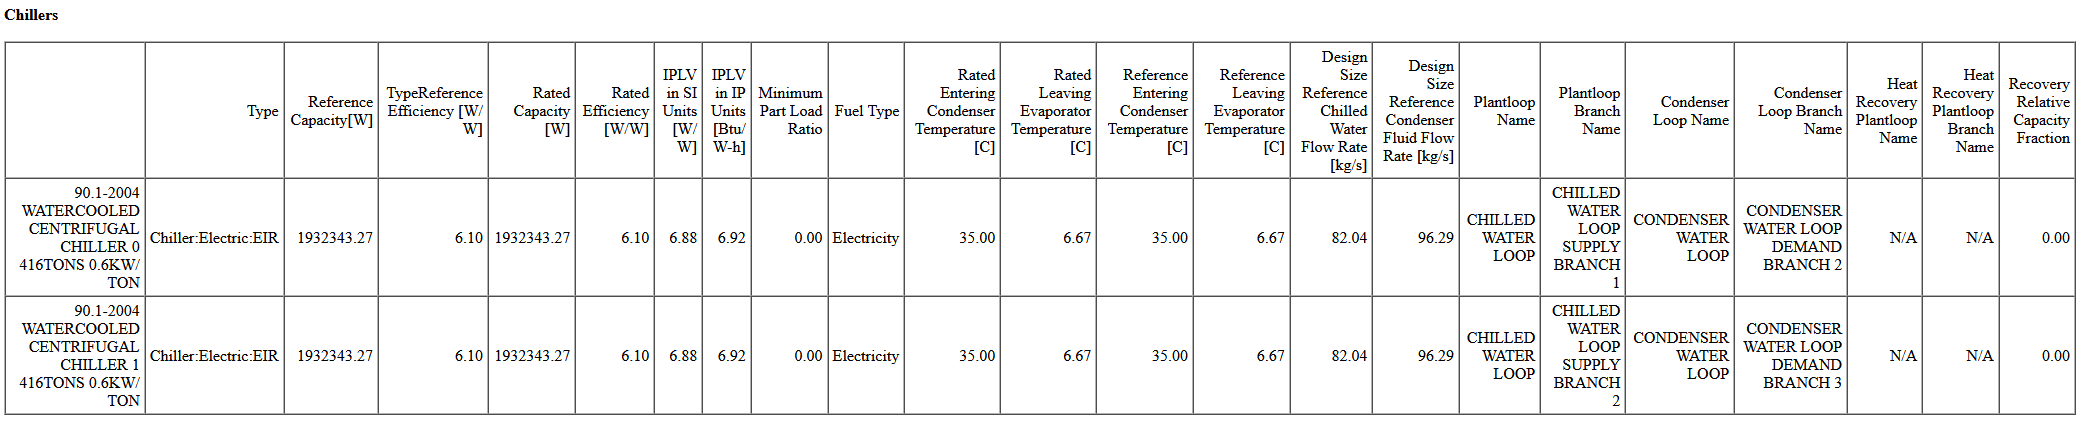
\includegraphics{media/chiller-table-example.PNG}
\caption{}
\end{figure}

Boilers

The columns for this report are shown below as a list:

\begin{itemize}
\item
	Type
\item
	Reference Capacity [W]
\item
	Reference Efficiency[W/W]
\item
	Rated Capacity [W]
\item
	Rated Efficiency [W/W]
\item
	Minimum Part Load Ratio
\item
	Fuel Type
\item
	Parasitic Electric Load [W]
\item
	Plantloop Name
\item
	Plantloop Branch Name
\end{itemize}

\begin{figure}[h!]
\centering
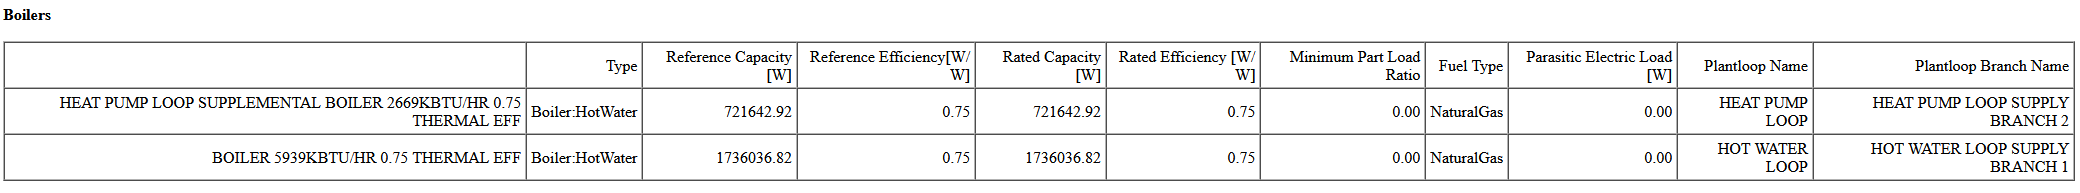
\includegraphics{media/boiler-table-example.PNG}
\caption{}
\end{figure}

Cooling Towers and Fluid Coolers

The columns for this report are shown below as a list:

\begin{itemize}
\item
	Type
\item
	Fluid Type
\item
	Range [C]
\item
	Approach [C]
\item
	Design Fan Power [W]
\item
	Design Inlet Air Wet-Bulb Temperature [C]
\item
	Design Water Flow Rate [m3/s]
\item
	Leaving Water Setpoint Temperature [C]
\item
	Condenser Loop Name
\item
	Condenser Loop Branch Name
\end{itemize}

\begin{figure}[h!]
\centering
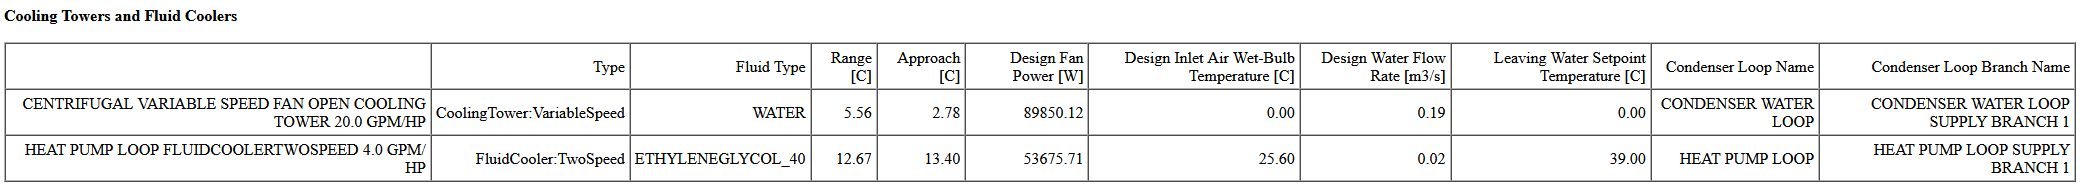
\includegraphics{media/cooling-tower-table-example.PNG}
\caption{}
\end{figure}

PlantLoop or CondenserLoop

The columns for this report are shown below as a list:

\begin{itemize}
\item
	Type
\item
	Provides Heating
\item
	Provides Cooling
\item
	Maximum Loop Flow Rate [m3/s]
\item
	Minimum Loop Flow Rate [m3/s]
\end{itemize}

\begin{figure}[h!]
\centering
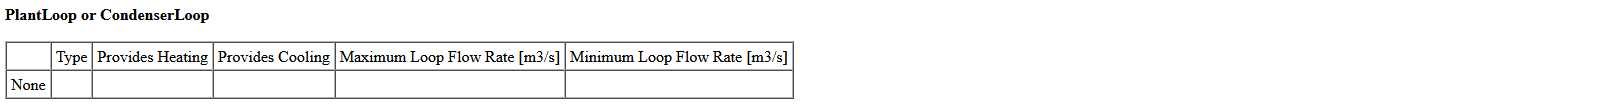
\includegraphics{media/plantloop-table-example.PNG}
\caption{}
\end{figure}

Air Terminals

The columns for this report are shown below as a list:

\begin{itemize}
\item
	Zone Name
\item
	Minimum Flow [m3/s]
\item
	Minimum Outdoor Flow [m3/s]
\item
	Supply Cooling Setpoint [C]
\item
	Supply Heating Setpoint [C]
\item
	Heating Capacity [W]
\item
	Cooling Capacity [W]
\item
	Type of Input Object
\item
	Heat/Reheat Coil Object Type
\item
	Chilled Water Coil Object Type
\item
	Fan Object Type
\item
	Fan Name
\item
	Primary Air Flow Rate [m3/s]
\item
	Secondary Air Flow Rate [m3/s]
\item
	Minimum Flow Schedule Name
\item
	Maximum Flow During Reheat [m3/s]
\item
	Minimum Outdoor Flow Schedule Name
\end{itemize}

\begin{figure}[h!]
\centering
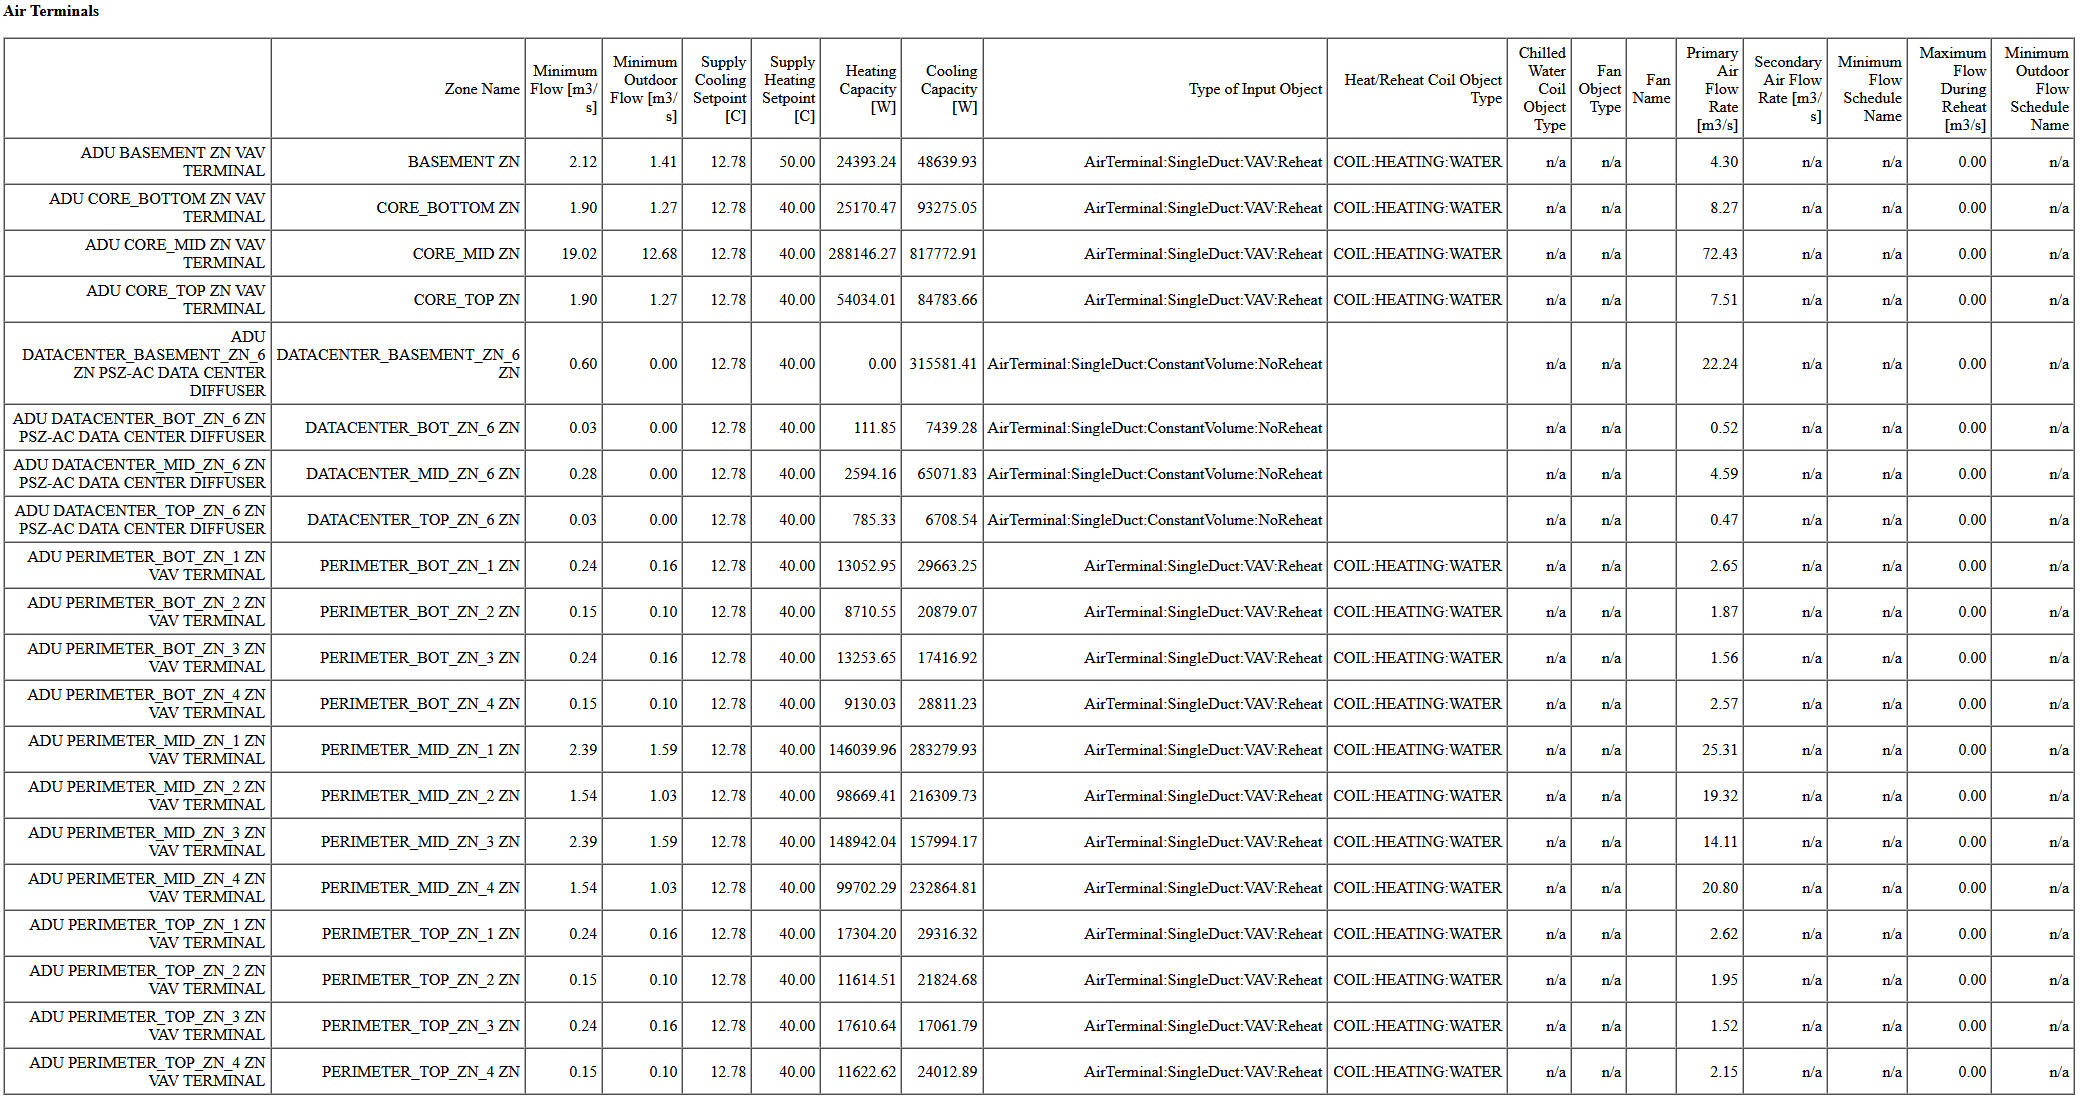
\includegraphics{media/air-terminal-table-example.PNG}
\caption{}
\end{figure}

Air Heat Recovery

The columns for this report are shown below as a list:

\begin{itemize}
\item
	Name
\item
	Input object type
\item
	Plate/Rotary
\item
	Sensible Effectiveness at 100% Heating Air Flow
\item
	Sensible Effectiveness at 100% Cooling Air Flow
\item
	Latent Effectiveness at 100% Heating Air Flow
\item
	Latent Effectiveness at 100% Cooling Air Flow
\item
	Exhaust Airflow [kg/s]
\item
	Outdoor Airflow [kg/s]
\end{itemize}


\begin{figure}[h!]
\centering
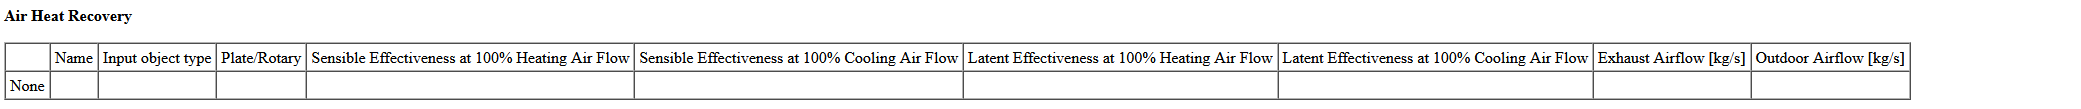
\includegraphics{media/air-heat-recovery-table-example.PNG}
\caption{}
\end{figure}


\subsection{Envelope Summary}\label{envelope-summary}

The Envelope Summary report provides a summary of the elements of the envelope of the building. The first table describes the exterior opaque elements and the second table describes the fenestration elements. Reflectance is defined as one minus the thermal absorptance. Directly following is an example of the report. The key used to obtain this report is EnvelopeSummary.

Report: Envelope Summary

For: Entire Facility

Timestamp: 2009-02-10 12:39:35

Opaque Exterior

{\scriptsize
\begin{longtable}[c]{>{\raggedright}p{0.6in}>{\raggedright}p{0.6in}>{\raggedright}p{0.6in}>{\raggedright}p{0.6in}>{\raggedright}p{0.6in}>{\raggedright}p{0.6in}>{\raggedright}p{0.6in}>{\raggedright}p{0.6in}>{\raggedright}p{0.6in}}
\toprule 
~ & Construction & Reflectance & U-Factor with Film (W/m2-K) & U-Factor no Film (W/m2-K) & Gross Area (m2) & Azimuth (deg) & Tilt (deg) & Cardinal Direction \tabularnewline
\midrule
\endfirsthead

\toprule 
~ & Construction & Reflectance & U-Factor with Film (W/m2-K) & U-Factor no Film (W/m2-K) & Gross Area (m2) & Azimuth (deg) & Tilt (deg) & Cardinal Direction \tabularnewline
\midrule
\endhead

WALL-1PF & WALL-1 & 0.22 & 0.384 & 0.41 & 18.30 & 210.00 & 90.00 & S \tabularnewline
WALL-1PR & WALL-1 & 0.22 & 0.384 & 0.41 & 9.12 & 120.00 & 90.00 & E \tabularnewline
WALL-1PB & WALL-1 & 0.22 & 0.384 & 0.41 & 18.30 & 30.00 & 90.00 & N \tabularnewline
WALL-1PL & WALL-1 & 0.22 & 0.384 & 0.41 & 9.12 & 300.00 & 90.00 & W \tabularnewline
TOP-1 & ROOF-1 & 0.35 & 0.268 & 0.28 & 463.60 & 210.00 & 0.00 & ~ \tabularnewline
FRONT-1 & WALL-1 & 0.22 & 0.384 & 0.41 & 73.20 & 210.00 & 90.00 & S \tabularnewline
F1-1 & FLOOR-SLAB-1 & 0.35 & 1.454 & 2.25 & 99.16 & 30.00 & 180.00 & ~ \tabularnewline
RIGHT-1 & WALL-1 & 0.22 & 0.384 & 0.41 & 36.48 & 120.00 & 90.00 & E \tabularnewline
F2-1 & FLOOR-SLAB-1 & 0.35 & 1.454 & 2.25 & 42.73 & 300.00 & 180.00 & ~ \tabularnewline
BACK-1 & WALL-1 & 0.22 & 0.384 & 0.41 & 73.20 & 30.00 & 90.00 & N \tabularnewline
F3-1 & FLOOR-SLAB-1 & 0.35 & 1.454 & 2.25 & 96.48 & 74.22 & 180.00 & ~ \tabularnewline
LEFT-1 & WALL-1 & 0.22 & 0.384 & 0.41 & 36.48 & 300.00 & 90.00 & W \tabularnewline
F4-1 & FLOOR-SLAB-1 & 0.35 & 1.454 & 2.25 & 42.73 & 120.00 & 180.00 & ~ \tabularnewline
F5-1 & FLOOR-SLAB-1 & 0.35 & 1.454 & 2.25 & 182.49 & 30.00 & 180.00 & ~ \tabularnewline
\bottomrule
\end{longtable}}

Exterior Fenestration

{\scriptsize
\begin{longtable}[c]{>{\raggedright}p{0.5in}>{\raggedright}p{0.5in}>{\raggedright}p{0.5in}>{\raggedright}p{0.5in}>{\raggedright}p{0.5in}>{\raggedright}p{0.5in}>{\raggedright}p{0.5in}>{\raggedright}p{0.5in}>{\raggedright}p{0.5in}>{\raggedright}p{0.5in}>{\raggedright}p{0.5in}}
\toprule 
~ & Construction & Area of One Opening (m2) & Area of Openings (m2) & U-Factor & SHGC & Visible Transmittance & Shade Control & Parent Surface & Azimuth (deg) & Cardinal Direction \tabularnewline
\midrule
\endfirsthead

\toprule 
~ & Construction & Area of One Opening (m2) & Area of Openings (m2) & U-Factor & SHGC & Visible Transmittance & Shade Control & Parent Surface & Azimuth (deg) & Cardinal Direction \tabularnewline
\midrule
\endhead

WF-1 & DBL CLR 3MM/13MM AIR & 16.56 & 16.56 & 2.72 & 0.763 & 0.812 & No & FRONT-1 & 210.00 & S \tabularnewline
DF-1 & SGL GREY 3MM & 6.00 & 6.00 & 5.89 & 0.708 & 0.611 & No & FRONT-1 & 210.00 & S \tabularnewline
WR-1 & DBL CLR 3MM/13MM AIR & 9.12 & 9.12 & 2.72 & 0.763 & 0.812 & No & RIGHT-1 & 120.00 & E \tabularnewline
WB-1 & DBL CLR 3MM/13MM AIR & 16.44 & 16.44 & 2.72 & 0.763 & 0.812 & No & BACK-1 & 30.00 & N \tabularnewline
DB-1 & SGL GREY 3MM & 4.41 & 4.41 & 5.89 & 0.708 & 0.611 & No & BACK-1 & 30.00 & N \tabularnewline
WL-1 & DBL CLR 3MM/13MM AIR & 9.12 & 9.12 & 2.72 & 0.763 & 0.812 & No & LEFT-1 & 300.00 & W \tabularnewline
Total or Average & ~ & ~ & 61.65 & 3.26 & 0.753 & 0.778 & ~ & ~ & ~ & ~ \tabularnewline
North Total or Average & ~ & ~ & 20.85 & 3.39 & 0.751 & 0.769 & ~ & ~ & ~ & ~ \tabularnewline
Non-North Total or Average & ~ & ~ & 40.80 & 3.19 & 0.755 & 0.782 & ~ & ~ & ~ & ~ \tabularnewline
\bottomrule
\end{longtable}}

The Exterior Fenestration table has been enhanced to show additional columns of data but an explicit example will not fit well on a page so instead the list of columns is shown below:

\begin{itemize}
\item
  Window Name
\item
  Construction
\item
  Glass Area [m2]
\item
  Frame Area [m2]
\item
  Divider Area [m2]
\item
  Area of One Opening [m2]
\item
  Area of Multiplied Openings [m2]
\item
  Glass U-Factor [W/m2-K]
\item
  Glass SHGC
\item
  Glass Visible Transmittance
\item
  Frame Conductance [W/m2-K]
\item
  Divider Conductance [W/m2-K]
\item
  NFRC Product Type
\item
  Assembly U-Factor [W/m2-K]
\item
  Assembly SHGC
\item
  Assembly Visible Transmittance
\item
  Shade Control (yes or no)
\item
  Parent Surface
\item
  Azimuth [deg]
\item
  Tilt [deg]
\item
  Cardinal Direction
\end{itemize}



Exterior Fenestration Shaded State


{\scriptsize
\begin{longtable}[c]{>{\raggedright}p{0.5in}>{\raggedright}p{0.5in}>{\raggedright}p{0.5in}>{\raggedright}p{0.5in}>{\raggedright}p{0.5in}>{\raggedright}p{0.5in}>{\raggedright}p{0.5in}>{\raggedright}p{0.5in}>{\raggedright}p{0.5in}>{\raggedright}p{0.5in}>{\raggedright}p{0.5in}}
\toprule 
~ & Glass U-Factor [W/m2-K] & Glass SHGC & Glass Visible Transmittance & Assembly U-Factor [W/m2-K] & Assembly SHGC & Assembly Visible Transmittance \tabularnewline
\midrule
\endfirsthead

\toprule 
~ & Glass U-Factor [W/m2-K] & Glass SHGC & Glass Visible Transmittance & Assembly U-Factor [W/m2-K] & Assembly SHGC & Assembly Visible Transmittance \tabularnewline
\midrule
\endhead

ELECTRO-CON-DARK & 2.560 & 0.710 & 0.113 & 2.742 & 0.207 & 0.108 \tabularnewline

\bottomrule
\end{longtable}}

Opaque Construction Layers

The columns for this report are shown as the ten possible layers of the construction, in order. An example of the report is shown.

\begin{figure}[h!]
\centering
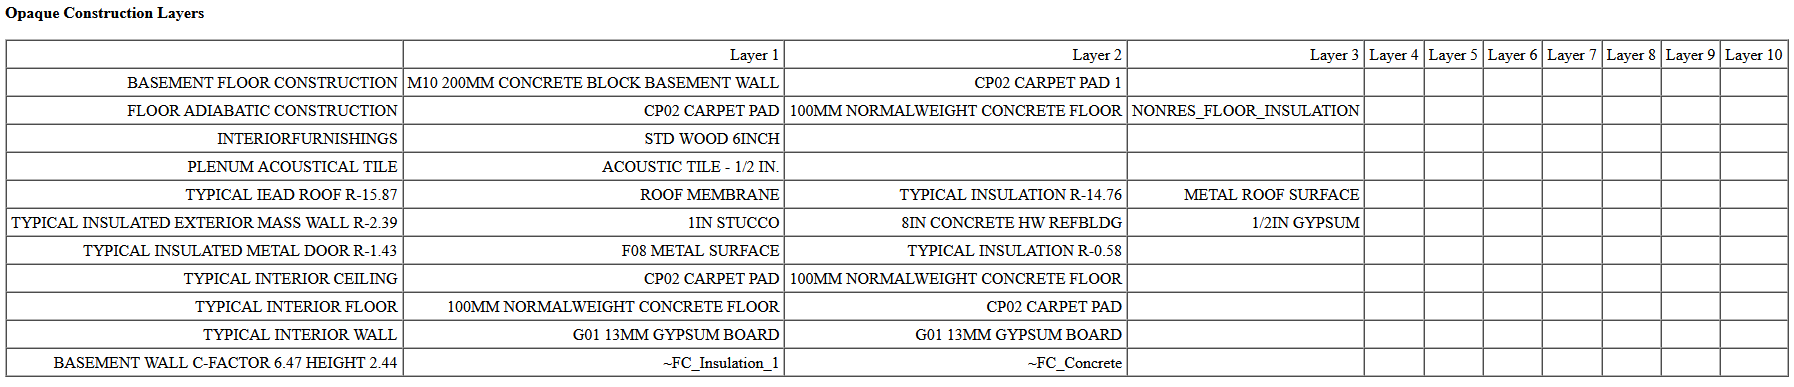
\includegraphics{media/layers-table-example.PNG}
\caption{}
\end{figure}




\subsection{Surface Shadowing Summary}\label{surface-shadowing-summary}

The Surface Shadowing Summary report summarizes how the surfaces may cast shadows on other surfaces. Directly following is an example of the report. The key used to obtain this report is SurfaceShadowingSummary.

Report: Surface Shadowing Summary

For: Entire Facility

Timestamp: 2007-10-17 08:54:27

Surfaces (Walls, Roofs, etc) that may be Shadowed by Other Surfaces

\begin{longtable}[c]{>{\raggedright}p{1.5in}>{\raggedright}p{4.5in}}
\toprule 
~ & Possible Shadow Casters \tabularnewline
\midrule
\endfirsthead

\toprule 
~ & Possible Shadow Casters \tabularnewline
\midrule
\endhead

FRONT-1 & MAIN SOUTH OVERHANG |Mir-MAIN SOUTH OVERHANG | \tabularnewline
SOUTH DOOR OVERHANG & Mir-MAIN SOUTH OVERHANG |WALL-1PF |FRONT-1 | \tabularnewline
WALL-1PF & Mir-MAIN SOUTH OVERHANG |SOUTH DOOR OVERHANG |Mir-SOUTH DOOR OVERHANG | \tabularnewline
MAIN SOUTH OVERHANG & FRONT-1 | \tabularnewline
\bottomrule
\end{longtable}

Subsurfaces (Windows and Doors) that may be Shadowed by Surfaces

\begin{longtable}[c]{@{}ll@{}}
\toprule 
~ & Possible Shadow Casters \tabularnewline
\midrule
\endfirsthead

\toprule 
~ & Possible Shadow Casters \tabularnewline
\midrule
\endhead

WF-1 & FRONT-1 | \tabularnewline
DF-1 & FRONT-1 | \tabularnewline
WR-1 & RIGHT-1 | \tabularnewline
WB-1 & BACK-1 | \tabularnewline
DB-1 & BACK-1 | \tabularnewline
WL-1 & LEFT-1 | \tabularnewline
\bottomrule
\end{longtable}

\subsection{Shading Summary}\label{shading-summary-000}

The Shading Summary report shows how much of each window is sunlit at different times of the year and also includes a summary of the window controls. Directly following is an example of the report. The key used to obtain this report is ShadingSummary.

Report: Shading Summary

For: Entire Facility

Timestamp: 2007-10-17 08:54:27

Sunlit Fraction

{\scriptsize
\begin{longtable}[c]{p{0.6in}p{0.6in}p{0.6in}p{0.6in}p{0.6in}p{0.6in}p{0.6in}p{0.6in}p{0.6in}p{0.6in}}
\toprule 
~ & March 21 9am & March 21 noon & March 21 3pm & June 21 9am & June 21 noon & June 21 3pm & December 21 9am & December 21 noon & December 21 3pm \tabularnewline
\midrule
\endfirsthead

\toprule 
~ & March 21 9am & March 21 noon & March 21 3pm & June 21 9am & June 21 noon & June 21 3pm & December 21 9am & December 21 noon & December 21 3pm \tabularnewline
\midrule
\endhead

WF-1 & 0.00 & 0.00 & 0.43 & 0.00 & 0.00 & 0.00 & 0.30 & 0.52 & 0.86 \tabularnewline
DF-1 & 0.73 & 0.26 & 0.62 & 0.00 & 0.00 & 0.28 & 0.90 & 0.69 & 0.92 \tabularnewline
WR-1 & 1.00 & 1.00 & 0.00 & 1.00 & 1.00 & 0.00 & 1.00 & 1.00 & 0.00 \tabularnewline
WB-1 & 0.00 & 0.00 & 0.00 & 1.00 & 0.00 & 0.00 & 0.00 & 0.00 & 0.00 \tabularnewline
DB-1 & 0.00 & 0.00 & 0.00 & 1.00 & 0.00 & 0.00 & 0.00 & 0.00 & 0.00 \tabularnewline
WL-1 & 0.00 & 0.00 & 1.00 & 0.00 & 0.00 & 1.00 & 0.00 & 0.00 & 1.00 \tabularnewline
\bottomrule
\end{longtable}}

Window Control

\begin{longtable}[c]{@{}llllll@{}}
\toprule 
~ & Name & Type & Shaded Construction & Control & Glare Control \tabularnewline
\midrule
\endfirsthead

\toprule 
~ & Name & Type & Shaded Construction & Control & Glare Control \tabularnewline
\midrule
\endhead

none & ~ & ~ & ~ & ~ & ~ \tabularnewline
\bottomrule
\end{longtable}

\subsection{Lighting Summary}\label{lighting-summary}

The Lighting Summary report provides a description of the interior and exterior lighting systems being simulated. It also provides a summary of daylighting controls. The Interior Lighting table has three columns that are explained below:

Scheduled Hours/Week {[}hr{]} - In the schedule shown, this represents the average weekly sum of hourly values. It is based on a full year even if the simulation is only performed for part of the year. It is not affected by daylighting.

Hours/Week \textgreater{} 1\% {[}hr{]} -- This represents the average hours per week that are above 1\% of the design value.

Full Load Hours/Week {[}hr{]} -- This is based on consumption and hours that the consumption occurred. It is dependent on the run period used. When simulating only a portion of the year, the value depends on which days of the year (the number of weekdays versus weekend days, for example) are simulated. It also indicates the impact of daylighting control. Directly following is an example of the report. The key used to obtain this report is LightingSummary.

Report: Lighting Summary

For: Entire Facility

Timestamp: 2012-09-05 12:10:52

Interior Lighting

{\scriptsize
\begin{longtable}[c]{>{\raggedright}p{0.46in}>{\raggedright}p{0.46in}>{\raggedright}p{0.46in}>{\raggedright}p{0.46in}>{\raggedright}p{0.46in}>{\raggedright}p{0.46in}>{\raggedright}p{0.46in}>{\raggedright}p{0.46in}>{\raggedright}p{0.46in}>{\raggedright}p{0.46in}>{\raggedright}p{0.46in}>{\raggedright}p{0.46in}>{\raggedright}p{0.46in}}
\toprule 
 & Zone & Lighting Power Density [W/m2] & Zone Area [m2] & Total Power [W] & End Use Subcategory & Schedule Name & Scheduled Hours/Week [hr] & Hours/Week  >  1\% [hr] & Full Load Hours/Week [hr] & Return Air Fraction & Conditioned (Y/N) & Consumption [GJ] \tabularnewline
\midrule
\endfirsthead

\toprule 
 & Zone & Lighting Power Density [W/m2] & Zone Area [m2] & Total Power [W] & End Use Subcategory & Schedule Name & Scheduled Hours/Week [hr] & Hours/Week  >  1\% [hr] & Full Load Hours/Week [hr] & Return Air Fraction & Conditioned (Y/N) & Consumption [GJ] \tabularnewline
\midrule
\endhead

SPACE1-1 LIGHTS 1 & SPACE1-1 & 15.9742 & 99.16 & 1584.00 & GeneralLights & LIGHTS-1 & 57.70 & 168.00 & 57.70 & 0.2000 & Y & 17.16 \tabularnewline
SPACE2-1 LIGHTS 1 & SPACE2-1 & 16.0056 & 42.73 & 684.00 & GeneralLights & HALFPERCENT & 0.60 & 0.00 & 0.59 & 0.2000 & Y & 0.08 \tabularnewline
SPACE3-1 LIGHTS 1 & SPACE3-1 & 16.4179 & 96.48 & 1584.00 & GeneralLights & ALWAYSON & 168.00 & 168.00 & 168.00 & 0.2000 & Y & 49.95 \tabularnewline
SPACE4-1 LIGHTS 1 & SPACE4-1 & 16.0056 & 42.73 & 684.00 & GeneralLights & LIGHTS-1 & 57.70 & 168.00 & 57.70 & 0.2000 & Y & 7.41 \tabularnewline
SPACE5-1 LIGHTS 1 & SPACE5-1 & 16.2420 & 182.49 & 2964.00 & GeneralLights & LIGHTS-1 & 57.70 & 168.00 & 57.70 & 0.2000 & Y & 32.11 \tabularnewline
Interior Lighting Total & ~ & 16.1777 & 463.60 & 7500.00 & ~ & ~ & ~ & ~ & ~ & ~ & ~ & 106.70 \tabularnewline
\bottomrule
\end{longtable}}

Daylighting

\begin{longtable}[c]{p{0.85in}p{0.85in}p{0.85in}p{0.85in}p{0.85in}p{0.85in}p{0.85in}}
\toprule 
 & Zone & Daylighting Type & Control Type & Fraction Controlled & Lighting Installed in Zone [W] & Lighting Controlled [W] \tabularnewline
\midrule
\endfirsthead

\toprule 
 & Zone & Daylighting Type & Control Type & Fraction Controlled & Lighting Installed in Zone [W] & Lighting Controlled [W] \tabularnewline
\midrule
\endhead

None & ~ & ~ & ~ & ~ & ~ & ~ \tabularnewline
\bottomrule
\end{longtable}

Exterior Lighting

\begin{longtable}[c]{>{\raggedright}p{0.75in}>{\raggedright}p{0.75in}>{\raggedright}p{0.75in}>{\raggedright}p{0.75in}>{\raggedright}p{0.75in}>{\raggedright}p{0.75in}>{\raggedright}p{0.75in}>{\raggedright}p{0.75in}}
\toprule 
 & Total Watts & Astronomical Clock/Schedule & Schedule Name & Scheduled Hours/Week [hr] & Hours/Week  >  1\% [hr] & Full Load Hours/Week [hr] & Consumption [GJ] \tabularnewline
\midrule
\endfirsthead

\toprule 
 & Total Watts & Astronomical Clock/Schedule & Schedule Name & Scheduled Hours/Week [hr] & Hours/Week  >  1\% [hr] & Full Load Hours/Week [hr] & Consumption [GJ] \tabularnewline
\midrule
\endhead

Exterior Lighting Total & 0.00 & ~ & ~ & ~ & ~ & ~ & 0.00 \tabularnewline
\bottomrule
\end{longtable}

\subsection{HVAC Sizing Summary}\label{hvac-sizing-summary}

The HVAC Sizing Summary report provides information on the zone cooling and heating sizing and the peak load conditions as well as information about the system air flow sizing. The Design Load is the zone sensible load only and it does not include any system effects or ventilation loads. The user specified design load and airflow and the values calculated by the program are shown in the report along with the time of the peak load and the temperature and humidity ratio at the time of the peak during the sizing periods. This information is generated for both the Zone Sensible Cooling and Zone Sensible Heating tables.

Also included is the System Design Air Flow Rates which includes the calculated cooling air flow rate, the user specified air flow rate for cooling, the calculated heating air flow rate, and the user specified air flow rate for heating.

\emph{Note:} values listed as ``calculated'' are the unaltered result of the zone or system sizing calculations, using the design sizing period weather and schedules specified in the input. Values listed as ``user specified'' are either the calculated values modified by global or zone sizing factors or values specified with the \emph{flow/zone} or \emph{flow/system} design air flow method.

The HVAC Sizing Summary also includes a coil summary report table. This is a large data table that collects a variety of results organized by each individual coil.  It can be viewed in html or csv format but it expected to be used from the sqlite database.  The table has 87 columns and a row for each coil in the building model.  The column titles are also called fields here, as in fields to use with a database query. 

Throughout this table the special value of -999.0 is deliberately used to signal that no data are available to report for that coil for that field or column.  This could be for a variety of reasons such as, no sizing calculations in the model, did not run design day full simulations, particular fields only applies to certain types of coils, certain calculations are only performed for particular coils, etc.  If you find a -999.0 in a situation where you think the value should be available, please report it.  Another special value of -99999.0 may be encountered which is used within EnergyPlus to signal that numeric input fields were set to Autosize, Autocalculate, or left blank and in some cases this value will carry into the coil report table.

The encyclopedic documentation that follows is important because in many cases, very similar data are available from up to three separate fields and one must be careful to understand the subtle differences and be aware that there is some repetition of the similar types of data in the fields.  This is mainly because coil performance changes with the conditions under which it operates and so an important part of this table is describing each coil under different sets of operating conditions.

There are three broad groupings of data fields in the table:

\begin{itemize}
\item
  Meta data.  The meta data fields include string names to identify the coil, where it is being used, names and types of IDF objects involved, what some of the various sizing method input choices were set to, and information about the supply fan and plant found to be associated with the coil.  40 fields. 
\item
  Ideal loads sizing summary. The collection of fields whose names end with ``at Ideal Loads Peak'' are all related to the sizing calculations done by the ideal loads zone sizing routines and the system sizing routines based on them.  Many of the values reported here come from Sizing:Zone and/or Sizing:System input.  The operating conditions occurring during Ideal Loads sizing calculations are unlikely to match the conditions used in the definitions for coil input data.  36 fields.
\item
  Rating point summary.  This is a collection of fields with names that end in ``at Rating Conditions.''  The model input data for many types of coils is based on defined set of conditions variously referred to as the rating point, reference, nominal, or design.  The coil models are calculated with conditions set to match the rating point and the inputs and outputs from that are reported here.  Many of the values here are from the input documentation that defines the conditions at the rating point. The coil capacities and leaving conditions are the results from the running complete coil model. Some coil models do not have a rating point as part of the model definition, because the models are not sensitive to operating conditions, and those coils will have -999.0 in these fields. 11 fields.
\end{itemize}

The following is a comprehensive listing of each column/field in the coil summary table with a brief definition and/or summary.

\emph{Coil Type} The input object class name in IDF syntax. Text string. 

\emph{Coil Location} The broad type of HVAC this coil is being used in.  ``AirLoop'' means the coil is part of a central air system, such as a main coil in a multizone air handler.  ``Zone Equipment'' means that the coil is part of Zone equipment like a PTAC, or in the zone terminal unit of an airhandler like a VAV reheat coil.   Text string.

\emph{HVAC Type} This is more specifically what HVAC the coil is used in. The values are the input object class name, in IDF syntax, found to be associated with the coil. Text string.

\emph{HVAC Name} This is the unique user name input for the \emph{HVAC Type}.  The strings  will be converted to upper case compared to what is in the actual input data file.  Text string.

\emph{Zone Name(s)} This is the zone, or list of zones, found to be associated with this coil.  The zone name is defined by the user in the Zone object.  For multizone systems, the coils can have a list of zone names with the individual names separated by a semicolon. The zones listed here are those used to generate (aggregate and volume-weighted average) values for the room conditions and loads. Text string. 

\emph{System Sizing Method Concurrence} This field applies to ``AirLoop'' coils.  It describes if the central air system sizing was done using ``Coincident'' or ``Non-Coincident'' method. This refers to how the ideal loads sizing routines process the time sequence of zone loads.  The concurrent sum of peaks, or coincident or ``block'', is often lower than the sum of the individual peaks regardless of when they occur, or non-coincident sum.  This field is not applicable to ``Zone Equipment'' coils and will show ``N/A'' here.  This corresponds to the input field called Type of Zone Sum to Use in the Sizing:System input object. Text string.

\emph{System Sizing Method Capacity} This field applies to ``AirLoop'' coils.  It describes what was chosen for the method of determining coil capacity during ideal loads sizing routines. The values here will match the input key choices available for the the Sizing:System object's input fields called \emph{Cooling Design Capacity Method}, for cooling coils, and \emph{Heating Design Capacity Method}, for heating coils. Values here of ``HeatingDesignCapacity'' or ``CoolingDesignCapacity'' mean that the coil was sized using the design loads calculated from the zone ideal loads results. When sizing was scaled using floor area the value here would be ``CapacityPerFloorArea.''  Values of \emph{FractionOfAutosizedHeatingCapacity} and \emph{FractionOfAutosizeCoolingCapacity} mean that the usual design load based results were further scaled by a separate user scaling factor. This field is not applicable to ``Zone Equipment'' coils and will show ``N/A'' here. Text string.

\emph{System Sizing Method Air Flow} This field applies to ``AirLoop'' coils.  It describes what was chosen for the method of determining the system air flow rate during ideal loads sizing routines. This field is not applicable to ``Zone Equipment'' coils and will show ``N/A'' here. Text string.

\emph{Autosized Coil Capacity?} This field describes if the coil capacity was autosized or not.  Values here will be ``Yes'' or ``No.''  A ``No'' means that the size of the coil was set at input, hard sized, and no capacity sizing calculations were done for the coil. A ``Yes'' means that coil's capacity was autosized. Text string.

\emph{Autosized Coil Airflow?} This field describes if the coil's airflow rate was autosized or not. Values here will be ``Yes'' or ``No.''  A ``No'' means that the airflow rate used to size the coil's capacity was set at input, hard sized.  This means that the coil's capacity was set for an airflow rate that was not autosized. A ``Yes'' means that the airflow rate for the coil came from sizing calculations. Text string.

\emph{Autosized Coil Water Flow?} This field describes if the coil's water flow rate was autosized or not. Values here will be ``Yes'' or ``No.''  A ``No'' means that the water flow rate used to size the coil's capacity was set at input, hard sized.  This means that the coil's capacity was set for a water flow rate that was not autosized. A ``Yes'' means that the water flow rate for the coil came from sizing calculations.  This field is only applicable to water-to-air coils. Text string.

\emph{OA Pretreated prior to coil inlet?} This field describes if the coil's sizing calculations are based on the outdoor air being preconditioned, as with a separate coil, or if the outdoor air is unconditioned. Values here will be ``Yes'' or ``No.''  A ``No'' means that the outdoor air is not preconditioned.  A ``Yes'' means that the outdoor is preconditioned.  This field only really applies to central air system coils.  The outdoor air may be mixed with return air before the coil, but that mixed air may be based on either treated or untreated outdoor air, depending on Sizing:System input.  Text string.

\emph{Coil Final Gross Total Capacity [W]} This field describes the coil's gross total capacity, in units of W.  No fan impact.  This field will generally be the main value the model uses for capacity as a result of the sizing calculations.  However if a coil was not autosized, the capacity was hard sized on input, then this field will be filled with the hard sized coil capacity (if that is a parameter in the coil model).  This field is very similar to the field called Coil Total Capacity at Rating Conditions with the difference being that this one is the model input while that other one is the result of running the full coil model at the rating point conditions.  Water heating coil models using UA and design water flow rate performance input method do not have a single design capacity in Watts and this field will show as -99999.0 (and the coil is better characterized using the field called Coil U-value Times Area Value).  Real number. 

\emph{Coil Final Gross Sensible Capacity [W]} Real number. This field describes the coil's gross sensible capacity, if available, in units of W. No fan impact.  This field is generally the total capacity multiplied by the sensible heat ratio if both are defined in the model. Real number.

\emph{Coil Final Reference Air Volume Flow Rate [m3/s]}  This field describes the coil's rated/reference/nominal air flow rate, in units of m3/s.  This field will generally be the model input (or autosize result) for the process air flow rate through the coil at the rating point.  Some coil models do not have any rated/reference/nominal air flow rate as part of the model description (d.g. electric and gas heating coils) and these will have -999.0 in this field. Real number. 

\emph{Coil Final Reference Plant Fluid Volume Flow Rate [m3/s]}  This field describes the coil's rated/reference/nominal water flow rate, in units of m3/s.  This field will be the model input or autosize result for the source water, or other plant fluid type, flow rate through the coil at the design or rating point.  Many coils have no water source and these will have -999.0 in this field.  Real number.

\emph{Coil U-value Times Area Value [W/K]} This field describes the coil's overall UA value, in units of W/K.  This is mainly for the Coil:Heating:Water coil using the Performance Input method of UFactorTimesAirAndDesignWaterFlowRate and is not available for other coils.  This will be the result from the ideal loads sizing calculations or the hard sized entry.  Real number.

\emph{Terminal Unit Reheat Coil Multiplier}  This field describes the coil sizing multiplier that might have affected the calculated size of a coil used as a reheat coil in a zone air terminal unit.  This is a non-dimensional scaling factor.  Real number.

\emph{DX Coil Capacity Increase Ratio from Too Low Flow/Capacity Ratio}  This field describes sizing adjustments that can occur for DX coils when the combination of capacity and air flow rate is outside of prescribed limits.  If the air flow to capacity ratio was too low this will ratio will show how the capacity was increased to force the result into the prescribed range.  Real Number.

\emph{DX Coil Capacity Decrease Ratio from Too High Flow/Capacity Ratio}  This field describes sizing adjustments that can occur for DX coils when the combination of capacity and air flow rate is outside of prescribed limits.  If the air flow to capacity ratio was too high this will ratio will show how the capacity was decreased to force the result into the prescribed range.  Real Number.

\emph{Moist Air Heat Capacity [J/kg-K]}  This is the moist air heat capacity, cp, that is applicable to coil calculations. Real number.

\emph{Dry Air Heat Capacity [J/kg-K]}  This is the dry air heat capacity, cp, that is applicable to coil calculations. Real number.

\emph{Standard Air Density Adjusted for Elevation [kg/m3]}  This is the dry air density, adjusted for elevation above sea level, that is applicable to coil calculations. Real number.

\emph{Supply Fan Name for Coil} The program tries to detect the supply fan associated with the coil.  This field is the user-defined name for that fan. Text string.

\emph{Supply Fan Type for Coil} The program tries to detect the supply fan associated with the coil. The values are the input object class name, in IDF syntax, for the fan.  Text string.

\emph{Supply Fan Maximum Air Volume Flow Rate [m3/s]}  This field is the design volume flow rate, in units of m3/s, for the fan found to be associated with the coil.  Real number

\emph{Supply Fan Maximum Air Mass Flow Rate [kg/s]} This field is the design mass flow rate, in kg/s, for the fan found to be associated with the coil. Real number

\emph{Plant Name for Coil} If the coil is a water-to-air or steam coil, then the program tries to detect the central plant system serving the coil. This field is the user-defined name for that plant system.  This will be the name in the PlantLoop and Sizing:Plant objects.  The next nine fields provides various results for that the central plant loop system.  If the coil is not a water or steam coil, then this field will have ``unknown'' as the value.  Text string.

\emph{Plant Fluid Specific Heat Capacity [J/kg-K]}  This is the specific heat of the fluid circulating through the plant and serving the coil, in units of J/kg-K.  This is evaluated at the temperature used for sizing calculations. The plant need not always be water, glycol mixtures and steam are supported and this value will be adjusted accordingly.  If the coil is not served by a plant, then this field will have -999.0 as the value. Real number.

\emph{Plant Fluid Density [kg/m3]} This is the density of the fluid circulating through the plant and serving the coil, in units of kg/m3.  This is evaluated at the temperature used for sizing calculations. The plant need not always be water, glycol mixtures are supported and this value will be adjusted accordingly.  If the coil is not served by a plant, then this field will have -999.0 as the value.  Real number.

\emph{Plant Maximum Fluid Mass Flow Rate [kg/s]}  This field is the design flow rate for the (entire) central plant system serving the coil, in units of kg/s.  This value is the final outcome from plant sizing calculations, or perhaps from the hard-sized value entered in the PlantLoop object for the maximum volume flow rate.  If the coil is not served by a plant, then this field will have -999.0 as the value. Real number.

\emph{Plant Design Fluid Return Temperature [C]}  This is the value, in degrees Celsius, used in sizing calculations for the temperature of the fluid returning to the supply side of the plant system.  It is derived from values entered in the Sizing:Plant object (except for steam which depends on subcooling input).  If the coil is not served by a plant, then this field will have -999.0 as the value. Real number.

\emph{Plant Design Fluid Supply Temperature [C]}  This is the value, in degrees Celsius, used in the sizing calculations for the temperature of the fluid leaving the supply side of the plant system and going into the coils.  This is the value entered in the Sizing:Plant object in the input field called Design Loop Exit Temperature (except for steam which is 100 C). If the coil is not served by a plant, then this field will have -999.0 as the value. Real number.

\emph{Plant Design Fluid Temperature Difference [Delta C]}  This is the value, in degrees Celsius (difference), used in the sizing calculations for the temperature difference between the plant supply and return temperatures.  This is the value entered in the Sizing:Plant object in the input field called Loop Design Temperature Difference (except for steam it is the amount of subcooling in the coil). If the coil is not served by a plant, then this field will have -999.0 as the value. Real number.

\emph{Plant Design Capacity [W]}  This is the design capacity of the central plant system, in Watts, that is the result of the sizing calculations.  For steam plants it is the capacity of the steam boiler attached to the supply side of the plant. If the coil is not served by a plant, then this field will have -999.0 as the value. Real number.

\emph{Coil Capacity Percentage of Plant Design Capacity [\%]}  The coil being reported on here will be one among many others that might be also be attached to the same plant.  This field compares this coil's (design gross) total capacity to the central plant's design capacity, W/W, and gives a value in percentage from 0.0 to 100.0.  If the coil is not served by a plant, then this field will have -999.0 as the value. Real Number.

\emph{Coil Fluid Flow Rate Percentage of Plant Design Flow Rate [\%]}  The coil being reported on here will be one among many others that might be also be attached to the same plant.  This field compares this coil's design flow rate to the central plant's design flow rate, {kg/s}/{kg/s}, and gives a value in percentage from 0.0 to 100.0.  If the coil is not served by a plant, then this field will have -999.0 as the value. Real Number.

\emph{Design Day Name at Sensible Ideal Loads Peak}  This field is the name of the design day selected to have the sensible load peak for ideal loads sizing calculations.  The text here will be from the user-defined names entered in the name field of the SizingPeriod:DesignDay objects.  If this is a cooling coil, the load peak will be for sensible cooling loads and the name here will be from one of the cooling design days.  If this is a heating coil, the load peak will be for sensible heating loads and the name from the heating design days.  Text String.

\emph{Date/Time at Sensible Ideal Loads Peak}  This field provides the result for the date and time of day when the sensible load peak was found to occur.  The format is (M)M/(D)D HH:MM:00, eg. 1/1 06:00:00 or 12/11 06:00:00.  There is no specific year associated with design days. Text String.

\emph{Design Day Name at Total Ideal Loads Peak}  The name of the design day selected to have the total load peak for ideal loads sizing calculations.  The text here will be from the user-defined names entered in the name field of the SizingPeriod:DesignDay objects.  If this is a cooling coil, the load peak will be for total cooling loads and the name here will be from one of the cooling design days.  If this is a heating coil, this field usually ``unknown'' because EnergyPlus does not use a total load for heating sizing. Text String.

\emph{Date/Time at Total Ideal Loads Peak}  This field provides the result for the date and time of day when the total load peak was found to occur during ideal loads sizing.  The format is (M)M/(D)D HH:MM:00, eg. 1/1 06:00:00 or 12/11 06:00:00.  There is no specific year associated with design days.  If the ideal loads sizing calculations never determine a total load the value here will be ``unknown.''  Text String.

\emph{Design Day Name at Air Flow Ideal Loads Peak}  This field is the name of the design day selected to have the air flow peak for ideal loads sizing calculations.  The text here will be from the user-defined names entered in the name field of the SizingPeriod:DesignDay objects.  If this is a cooling coil, the air flow peak might be calculated separately and the name here will be from one of the cooling design days.  If this is a heating coil, the air flow peak will be the same as the sensible load peak.  Text String.

\emph{Date/Time at Air Flow Ideal Loads Peak}  This field provides the result for the date and time of day when the air flow peak was found to occur.  The format is (M)M/(D)D HH:MM:00, eg. 1/1 06:00:00 or 12/11 06:00:00.  There is no specific year associated with design days. Text String.

\emph{Coil Total Capacity at Ideal Loads Peak [W]}  This field is the coil's gross total capacity, in Watts, resulting from the ideal loads sizing calculations.  This is the total, sensible plus latent, capacity under the conditions used for ideal loads sizing described in other ``Ideal Loads Peak'' fields.  This does not include the supply fan impacts.  Real Number.

\emph{Coil Sensible Capacity at Ideal Loads Peak [W]}  This field is the coil's gross sensible capacity, in Watts, resulting from the ideal loads sizing calculations.  This is the sensible capacity under the conditions used for ideal loads sizing described in the other ``Ideal Loads Peak'' fields.  This does not include the supply fan impacts.  Real number.

\emph{Coil Off-Rating Capacity Modifier at Ideal Loads Peak [ ]}  This field is the capacity modification factor for the conditions during ideal loads sizing.  The coil model may have performance curves that alter the capacity as a function of the conditions experienced by the coil. When the ideal loads sizing conditions are different than the conditions that the performance curves are normalized to, the rating point, the coil is being sized at ``Off-rating.''  This value can be used to convert the Coil Total Capacity at Ideal Loads Peak to what the capacity should be at the rating point.  The ideal loads sizing is often not at the rating point because of a fraction of outdoor air has been mixed into the entering air. Real number.

\emph{Coil Air Mass Flow Rate at Ideal Loads Peak [kg/s]}  This field is the coil's air mass flow rate, in kg/s, resulting from, and/or used during, the ideal loads sizing calculations.  Real number.

\emph{Coil Air Volume Flow Rate at Ideal Loads Peak [m3/s]}  This field is the coil's air volume flow rate, in m3/s, resulting from, and/or used during, the ideal loads sizing calculations.  Real number.

\emph{Coil Entering Air Drybulb at Ideal Loads Peak [C]}  This field is the drybulb temperature, in degrees Celsius, of the air entering the coil during ideal loads sizing calculations.  Real number.

\emph{Coil Entering Air Wetbulb at Ideal Loads Peak [C]}  This field is the wetbulb temperature, in degrees Celsius, of the air entering the coil during ideal loads sizing calculations.  Real number.

\emph{Coil Entering Air Humidity Ratio at Ideal Loads Peak [kg-H2O/kg-DryAir]}  This field is the humidity ratio, in kg-water/kg-dryAir, of the air entering the coil during ideal loads sizing calculations. Real number.

\emph{Coil Entering Air Enthalpy at Ideal Loads Peak [J/(kg-K)]}  This field is the enthalpy, in J/kg-K (base 0.0 at drybulb = 0.0$^\circ$C), of the air entering the coil during ideal loads sizing calculations. Real number.

\emph{Coil Leaving Air Drybulb at Ideal Loads Peak [C]}  This field is the drybulb temperature, in degrees Celsius, of the air leaving the coil during the ideal loads sizing calculations for the coil.  Real number.

\emph{Coil Leaving Air Wetbulb at Ideal Loads Peak [C]}  This field is the wetbulb temperature, in degrees Celsius, of the air leaving the coil during ideal loads sizing calculations. Real number.

\emph{Coil Leaving Air Humidity Ratio at Ideal Loads Peak [C]}  This field is the humidity ratio, in kg-water/kg-dryAir, of the air leaving the coil during ideal loads sizing calculations. Real number.

\emph{Coil Leaving Air Enthalpy at Ideal Loads Peak [J/(kg-K)]}  This field is the enthalpy, in J/kg-K (base 0.0 at drybulb = 0.0$^\circ$C), of the air leaving the coil during ideal loads sizing calculations. Real number.

\emph{Coil Plant Fluid Mass Flow Rate at Ideal Loads Peak [kg/s]}  This field is the design or maximum water flow rate, in kg/s, of the plant fluid serving the coil during ideal loads sizing calculations.  If the coil is not a water coil then this field will have a value of -999.0. Real number.

\emph{Coil Entering Plant Fluid Temperature at Ideal Loads Peak [C]}  This field is the water temperature, in degrees Celsius, of the plant fluid entering the coil during ideal loads sizing calculations.  If the coil is not a water coil then this field will have a value of -999.0. Real number.

\emph{Coil Leaving Plant Fluid Temperature at Ideal Loads Peak [C]}  This field is the water temperature, in degrees Celsius, of the plant fluid leaving the coil during ideal loads sizing calculations.  If the coil is not a water coil then this field will have a value of -999.0. Real number.

\emph{Coil Plant Fluid Temperature Difference at Ideal Loads Peak [Delta C]}  This field is the water temperature difference across the coil, in degrees Celsius (difference), of the plant fluid passing through the coil during ideal loads sizing calculations.  If the coil is not a water coil then this field will have a value of -999.0. Real number.

\emph{Supply Fan Air Heat Gain at Ideal Loads Peak [W]}  This field is the fan load that was included in the ideal loads sizing calculations.  This may only be included in calculations for central air system cooling coils.  If the coil was not sized with fan heat gain taken into account, then this value will be 0.0 (even though there still is a fan with heat during normal operation).  Real number.

\emph{Coil and Fan Net Total Capacity at Ideal Loads Peak [W]}  This field shows the net coil total capacity which is the gross total capacity with the fan heat gain, if any was calculated.  Real number.

\emph{Outdoor Air Drybulb at Ideal Loads Peak [C]}  This field is the outdoor air drybulb temperature, in degrees Celsius, used during the ideal loads sizing calculations.  Real number.

\emph{Outdoor Air Humidity Ratio at Ideal Loads Peak [kg-H2O/kg-DryAir]} This field is the outdoor air humidity ratio, in kg of water per kg of dry air, used during the ideal loads sizing calculations.  Real number.

\emph{Outdoor Air Wetbulb at Ideal Loads Peak [C]}  This field is the outdoor air wetbulb temperature, in degrees Celsius, used during the ideal loads sizing calculations.  Real number.

\emph{Outdoor Air Volume Flow Rate at Ideal Loads Peak [m3/s]}  This field is the outdoor air volume flow rate, in m3/s, that occurred during the ideal loads sizing calculations. Real number.

\emph{Outdoor Air Flow Percentage at Ideal Loads Peak [\%]}  This field is the percentage of outdoor air in the air entering the coil that occurred during the ideal loads sizing calculations. Real number.

\emph{System Return Air Drybulb at Ideal Loads Peak [C]}  This field is the drybulb temperature, in degrees C, of air returning into the HVAC system that occurred during the ideal loads sizing calculations. Real number.

\emph{System Return Air Humidity Ratio at Ideal Loads Peak [kg-H2O/kg-DryAir]}  This field is the humidity ratio, in kg of water per kg of dry air, of air returning into the HVAC system that occurred during the ideal loads sizing calculations. Real number.

\emph{Zone Air Drybulb at Ideal Loads Peak [C]}  This field is the drybulb temperature, in degrees C, of the zone air that occurred during the ideal loads sizing calculations. For multizone system this is the supply-air-volume-flow-weighted average. Real number.

\emph{Zone Air Humidity Ratio at Ideal Loads Peak [kg-H2O/kg-DryAir]}  This field is the humidity ratio, in kg of water per kg of dry air, of the zone air that occurred during the ideal loads sizing calculations. For multizone system this is the supply-air-volume-flow-weighted-weighted average. Real number.

\emph{Zone Air Relative Humidity at Ideal Loads Peak [\%]}  This field is the percent relative humidity of the zone air that occurred during the ideal loads sizing calculations. For multizone system this is the supply-air-volume-flow-weighted-weighted average. Real number.

\emph{Zone Sensible Heat Gain at Ideal Loads Peak [W]}  This field is the zone sensible load, in Watts, found during ideal loads sizing.  For multizone system it is the sum of all the zones on the air system. Real number.

\emph{Zone Latent Heat Gain at Ideal Loads Peak [W]}  This field is the zone latent load, in Watts, found during ideal loads sizing.  For multizone system it is the sum of all the zones on the air system. Real number.

\emph{Coil Total Capacity at Rating Conditions [W]}  This field is the gross total capacity of the coil when operated at the rating point conditions, in units of Watts.  This is the result from calculating the full coil model under the operating conditions specified for the rating point.  Real number.

\emph{Coil Sensible Capacity at Rating Conditions [W]}  This field is the gross sensible capacity of the coil when operated at the rating point conditions, in units of Watts.  This is the result from calculating the full coil model under the operating conditions specified for the rating point.  Real number.

\emph{Coil Air Mass Flow Rate at Rating Conditions [kg/s]}  This field is the air mass flow rate, in units of kg/s, used when calculating the full coil model under the operating conditions specified for the rating point.  Real number.

\emph{Coil Entering Air Drybulb at Rating Conditions [C]}  This field is the coil air inlet drybulb temperature, in degrees Celsius, used when calculating the full coil model under the operating conditions specified for the rating point.  The value should match the definition of the rating point as described in the coil model input documentation.  For DX cooling coils, this will be 26.6667C or 80F.  Real number.

\emph{Coil Entering Air Wetbulb at Rating Conditions [C]}  This field is the coil air inlet wetbulb temperature, in degrees Celsius, used when calculating the full coil model under the operating conditions specified for the rating point.  The value should match the definition of the rating point as described in the coil model input documentation.  For DX cooling coils, this will be 19.444C or 67F. Real number

\emph{Coil Entering Air Humidity Ratio at Rating Conditions [kg-H2O/kg-DryAir]}  This field is the coil air inlet humidity ratio, in kg-water/kg-dryAir, used when calculating the full coil model under the operating conditions specified for the rating point.  Real number.

\emph{Coil Entering Air Enthalpy at Rating Conditions [J/(kg-K)]}  This field is the coil air inlet enthalpy, in J/kg-K with zero base at 0.0$^\circ$C, used when calculating the full coil model under the operating conditions specified for the rating point. Real number.

\emph{Coil Leaving Air Drybulb at Rating Conditions [C]}  This field is the coil air outlet drybulb, in degrees Celsius, from calculating the full coil model under the operating conditions specified for the rating point. Real number.

\emph{Coil Leaving Air Wetbulb at Rating Conditions [C]}  This field is the coil air outlet wetbulb, in degrees Celsius, from calculating the full coil model under the operating conditions specified for the rating point. Real number.

\emph{Coil Leaving Air Humidity Ratio at Rating Conditions [kg-H2O/kg-DryAir]}  This field is the coil air outlet humidity ratio, in kg-water/kg-dryair, from calculating the full coil model under the operating conditions specified for the rating point. Real number.

\emph{Coil Leaving Air Enthalpy at Rating Conditions [J/(kg-K)]} This field is the coil air outlet enthalpy, in J/kg-K with zero base at 0.0$^\circ$C, from calculating the full coil model under the operating conditions specified for the rating point. Real number.
Directly following is an example of the report.

The key used to obtain this report is HVACSizingSummary.

Report: \textbf{HVAC Sizing Summary}

For: \textbf{Entire Facility}

** Timestamp: **2011-09-23 15:09:34

\textbf{Zone Sensible Cooling}

{\scriptsize
\begin{longtable}[c]{>{\raggedright}p{0.66in}>{\raggedright}p{0.66in}>{\raggedright}p{0.66in}>{\raggedright}p{0.66in}>{\raggedright}p{0.66in}>{\raggedright}p{0.66in}>{\raggedright}p{0.66in}>{\raggedright}p{0.66in}>{\raggedright}p{0.66in}}
\toprule 
 & Calculated Design Load [W] & User Design Load [W] & Calculated Design Air Flow [m3/s] & User Design Air Flow [m3/s] & Design Day Name & Date/Time Of Peak & Temperature at Peak [C] & Humidity Ratio at Peak [kgWater/kgAir] \tabularnewline
\midrule
\endfirsthead

\toprule 
 & Calculated Design Load [W] & User Design Load [W] & Calculated Design Air Flow [m3/s] & User Design Air Flow [m3/s] & Design Day Name & Date/Time Of Peak & Temperature at Peak [C] & Humidity Ratio at Peak [kgWater/kgAir] \tabularnewline
\midrule
\endhead

SPACE1-1 & 2647.33 & 2647.33 & 0.223 & 0.223 & CHICAGO\-\_IL\-\_USA ANNUAL COOLING 1\% DESIGN CONDITIONS DB/MCWB & 7/21 15:45:00 & 31.02 & 0.01459 \tabularnewline
SPACE2-1 & 2234.38 & 2234.38 & 0.188 & 0.188 & CHICAGO\-\_IL\-\_USA ANNUAL COOLING 1\% DESIGN CONDITIONS DB/MCWB & 7/21 10:00:00 & 27.43 & 0.01459 \tabularnewline
SPACE3-1 & 2506.34 & 2506.34 & 0.211 & 0.211 & CHICAGO\-\_IL\-\_USA ANNUAL COOLING 1\% DESIGN CONDITIONS DB/MCWB & 7/21 15:00:00 & 31.50 & 0.01459 \tabularnewline
SPACE4-1 & 2464.72 & 2464.72 & 0.207 & 0.207 & CHICAGO\-\_IL\-\_USA ANNUAL COOLING 1\% DESIGN CONDITIONS DB/MCWB & 7/21 17:30:00 & 29.47 & 0.01459 \tabularnewline
SPACE5-1 & 2628.69 & 2628.69 & 0.221 & 0.221 & CHICAGO\-\_IL\-\_USA ANNUAL COOLING 1\% DESIGN CONDITIONS DB/MCWB & 7/21 15:00:00 & 31.50 & 0.01459 \tabularnewline
\bottomrule
\end{longtable}}

\textbf{Zone Sensible Heating}

{\scriptsize
\begin{longtable}[c]{>{\raggedright}p{0.66in}>{\raggedright}p{0.66in}>{\raggedright}p{0.66in}>{\raggedright}p{0.66in}>{\raggedright}p{0.66in}>{\raggedright}p{0.66in}>{\raggedright}p{0.66in}>{\raggedright}p{0.66in}>{\raggedright}p{0.66in}}
\toprule 
 & Calculated Design Load [W] & User Design Load [W] & Calculated Design Air Flow [m3/s] & User Design Air Flow [m3/s] & Design Day Name & Date/Time Of Peak & Temperature at Peak [C] & Humidity Ratio at Peak [kgWater/kgAir] \tabularnewline
\midrule
\endfirsthead

\toprule 
 & Calculated Design Load [W] & User Design Load [W] & Calculated Design Air Flow [m3/s] & User Design Air Flow [m3/s] & Design Day Name & Date/Time Of Peak & Temperature at Peak [C] & Humidity Ratio at Peak [kgWater/kgAir] \tabularnewline
\midrule
\endhead

SPACE1-1 & 3860.76 & 3860.76 & 0.117 & 0.117 & CHICAGO\-\_IL\-\_USA ANNUAL HEATING 99\% DESIGN CONDITIONS DB & 1/21 24:00:00 & -17.30 & 0.00084 \tabularnewline
SPACE2-1 & 1625.15 & 1625.15 & 0.049 & 0.049 & CHICAGO\-\_IL\-\_USA ANNUAL HEATING 99\% DESIGN CONDITIONS DB & 1/21 24:00:00 & -17.30 & 0.00084 \tabularnewline
SPACE3-1 & 3753.07 & 3753.07 & 0.113 & 0.113 & CHICAGO\-\_IL\-\_USA ANNUAL HEATING 99\% DESIGN CONDITIONS DB & 1/21 24:00:00 & -17.30 & 0.00084 \tabularnewline
SPACE4-1 & 1625.15 & 1625.15 & 0.049 & 0.049 & CHICAGO\-\_IL\-\_USA ANNUAL HEATING 99\% DESIGN CONDITIONS DB & 1/21 24:00:00 & -17.30 & 0.00084 \tabularnewline
SPACE5-1 & 2981.57 & 2981.57 & 0.090 & 0.103 & CHICAGO\-\_IL\-\_USA ANNUAL HEATING 99\% DESIGN CONDITIONS DB & 1/21 24:00:00 & -17.30 & 0.00084 \tabularnewline
\bottomrule
\end{longtable}}

\textbf{System Design Air Flow Rates}

\begin{longtable}[c]{>{\raggedright}p{1.2in}>{\raggedright}p{1.2in}>{\raggedright}p{1.2in}>{\raggedright}p{1.2in}>{\raggedright}p{1.2in}}
\toprule 
 & Calculated cooling [m3/s] & User cooling [m3/s] & Calculated heating [m3/s] & User heating [m3/s] \tabularnewline
\midrule
\endfirsthead

\toprule 
 & Calculated cooling [m3/s] & User cooling [m3/s] & Calculated heating [m3/s] & User heating [m3/s] \tabularnewline
\midrule
\endhead

VAV SYS 1 & 1.05 & 1.05 & 0.43 & 0.43 \tabularnewline
\bottomrule
\end{longtable}

\textbf{Plant Loop Coincident Design Fluid Flow Rate Adjustments}

{\scriptsize
\begin{longtable}[c]{>{\raggedright}p{0.66in}>{\raggedright}p{0.66in}>{\raggedright}p{0.66in}>{\raggedright}p{0.66in}>{\raggedright}p{0.66in}>{\raggedright}p{0.66in}>{\raggedright}p{0.66in}>{\raggedright}p{0.66in}>{\raggedright}p{0.66in}}
\toprule 
 & Previous Design Volume Flow Rate [m3/s] & Algorithm Volume Flow Rate [m3/s] & Coincident Design Volume Flow Rate [m3/s] & Coincident Size Adjusted & Peak Sizing Period Name & Peak Day into Period & Peak Hour Of Day & Peak Step Start Minute \tabularnewline
\midrule
\endfirsthead

\toprule 
 & Previous Design Volume Flow Rate [m3/s] & Algorithm Volume Flow Rate [m3/s] & Coincident Design Volume Flow Rate [m3/s] & Coincident Size Adjusted & Peak Sizing Period Name & Peak Day into Period & Peak Hour Of Day & Peak Step Start Minute \tabularnewline
\midrule
\endhead

COOLSYS1 Sizing Pass 1 & 0.120672 & 0.141525 & 0.141525 & Yes & CHICAGO ANN CLG .4\% CONDNS WB= > MDB HVAC Sizing Pass 1 & 1 & 2 & 30 > \tabularnewline
HEATSYS1 Sizing Pass 1 & 0.060598 & 0.049054 & 0.049054 & Yes & CHICAGO ANN HTG 99.6\% CONDNS DB HVAC Sizing Pass 1 & 1 & 7 & 20 > \tabularnewline
\bottomrule
\end{longtable}}

\subsection{System Summary}\label{system-summary}

The System Summary report provides information about some of the primary components in the system including the economizer and demand controlled ventilation. In addition, this report describes when the zone conditions are not comfortable or when set points are not met.

In the \emph{Time Not Comfortable Based on Simple ASHRAE 55-2004} and Time Setpoint Not Met sub-tables, The reported time represents the total number of hours that a given zone did not meet the comfort or setpoint criteria. For the Facility row, this is the total numbers of hours that one or more zones were out of range. The values are not weighted by number of zones or number of occupants.

Directly following is an example of the report. The key used to obtain this report is SystemSummary.

Report: System Summary

For: Entire Facility

Timestamp: 2007-10-17 08:54:27

Economizer

\begin{longtable}[c]{>{\raggedright}p{0.75in}>{\raggedright}p{0.75in}>{\raggedright}p{0.75in}>{\raggedright}p{0.75in}>{\raggedright}p{0.75in}>{\raggedright}p{0.75in}>{\raggedright}p{0.75in}>{\raggedright}p{0.75in}}
\toprule 
~ & High Limit Shutoff Control & Minimum Outside Air (m3/s) & Maximum Outside Air (m3/s) & Return Air Temp Limit & Return Air Enthalpy Limit & Outside Air Temperature Limit (C) & Outside Air Enthalpy Limit (C) \tabularnewline
\midrule
\endfirsthead

\toprule 
~ & High Limit Shutoff Control & Minimum Outside Air (m3/s) & Maximum Outside Air (m3/s) & Return Air Temp Limit & Return Air Enthalpy Limit & Outside Air Temperature Limit (C) & Outside Air Enthalpy Limit (C) \tabularnewline
\midrule
\endhead

none & ~ & ~ & ~ & ~ & ~ & ~ & ~ \tabularnewline
\bottomrule
\end{longtable}

Demand Controlled Ventilation using VENTILATION:MECHANICAL

\begin{longtable}[c]{>{\raggedright}p{1.5in}>{\raggedright}p{1.5in}>{\raggedright}p{1.5in}>{\raggedright}p{1.5in}}
\toprule 
~ & Ventilation:Mechanical Name & Outside Air Per Person(m3/s-person) & Outside Air Per Area (m3/s-m2) \tabularnewline
\midrule
\endfirsthead

\toprule 
~ & Ventilation:Mechanical Name & Outside Air Per Person(m3/s-person) & Outside Air Per Area (m3/s-m2) \tabularnewline
\midrule
\endhead

none & ~ & ~ & ~ \tabularnewline
\bottomrule
\end{longtable}

Time Not Comfortable Based on Simple ASHRAE 55-2004

\begin{longtable}[c]{>{\raggedright}p{1.5in}>{\raggedright}p{1.5in}>{\raggedright}p{1.5in}>{\raggedright}p{1.5in}}
\toprule 
~ & Winter Clothes (hr) & Summer Clothes (hr) & Summer or Winter Clothes (hr) \tabularnewline
\midrule
\endfirsthead

\toprule 
~ & Winter Clothes (hr) & Summer Clothes (hr) & Summer or Winter Clothes (hr) \tabularnewline
\midrule
\endhead

SPACE1-1 & 429.00 & 1913.75 & 79.25 \tabularnewline
SPACE2-1 & 739.25 & 1719.75 & 22.50 \tabularnewline
SPACE3-1 & 482.00 & 1885.50 & 85.50 \tabularnewline
SPACE4-1 & 588.25 & 2039.75 & 59.50 \tabularnewline
SPACE5-1 & 14.75 & 2535.75 & 14.75 \tabularnewline
PLENUM-1 & 0.00 & 0.00 & 0.00 \tabularnewline
Facility & 1041.75 & 2564.75 & 97.00 \tabularnewline
\bottomrule
\end{longtable}

Time Setpoint Not Met

\begin{longtable}[c]{>{\raggedright}p{1.2in}>{\raggedright}p{1.2in}>{\raggedright}p{1.2in}>{\raggedright}p{1.2in}>{\raggedright}p{1.2in}}
\toprule 
~ & During Heating (hr) & During Cooling (hr) & During Occupied Heating (hr) & During Occupied Cooling (hr) \tabularnewline
\midrule
\endfirsthead

\toprule 
~ & During Heating (hr) & During Cooling (hr) & During Occupied Heating (hr) & During Occupied Cooling (hr) \tabularnewline
\midrule
\endhead

SPACE1-1 & 321.00 & 45.25 & 35.00 & 45.25 \tabularnewline
SPACE2-1 & 104.25 & 44.00 & 0.25 & 10.75 \tabularnewline
SPACE3-1 & 297.50 & 0.75 & 36.25 & 0.75 \tabularnewline
SPACE4-1 & 77.75 & 27.00 & 0.25 & 0.00 \tabularnewline
SPACE5-1 & 292.25 & 1.00 & 13.75 & 1.00 \tabularnewline
PLENUM-1 & 0.00 & 0.00 & 0.00 & 0.00 \tabularnewline
Facility & 333.50 & 117.00 & 37.25 & 56.75 \tabularnewline
\bottomrule
\end{longtable}

Thermostat Schedules

The columns for this report are shown below as a list:

\begin{itemize}
\item
  Thermostat Name 1
\item
  Control Type Schedule
\item
  Control Type
\item
  Control Type Name
\item
  Heating Schedule
\item
  Cooling Schedule
\end{itemize}

An example of the report is shown here

\begin{figure}[h!]
\centering
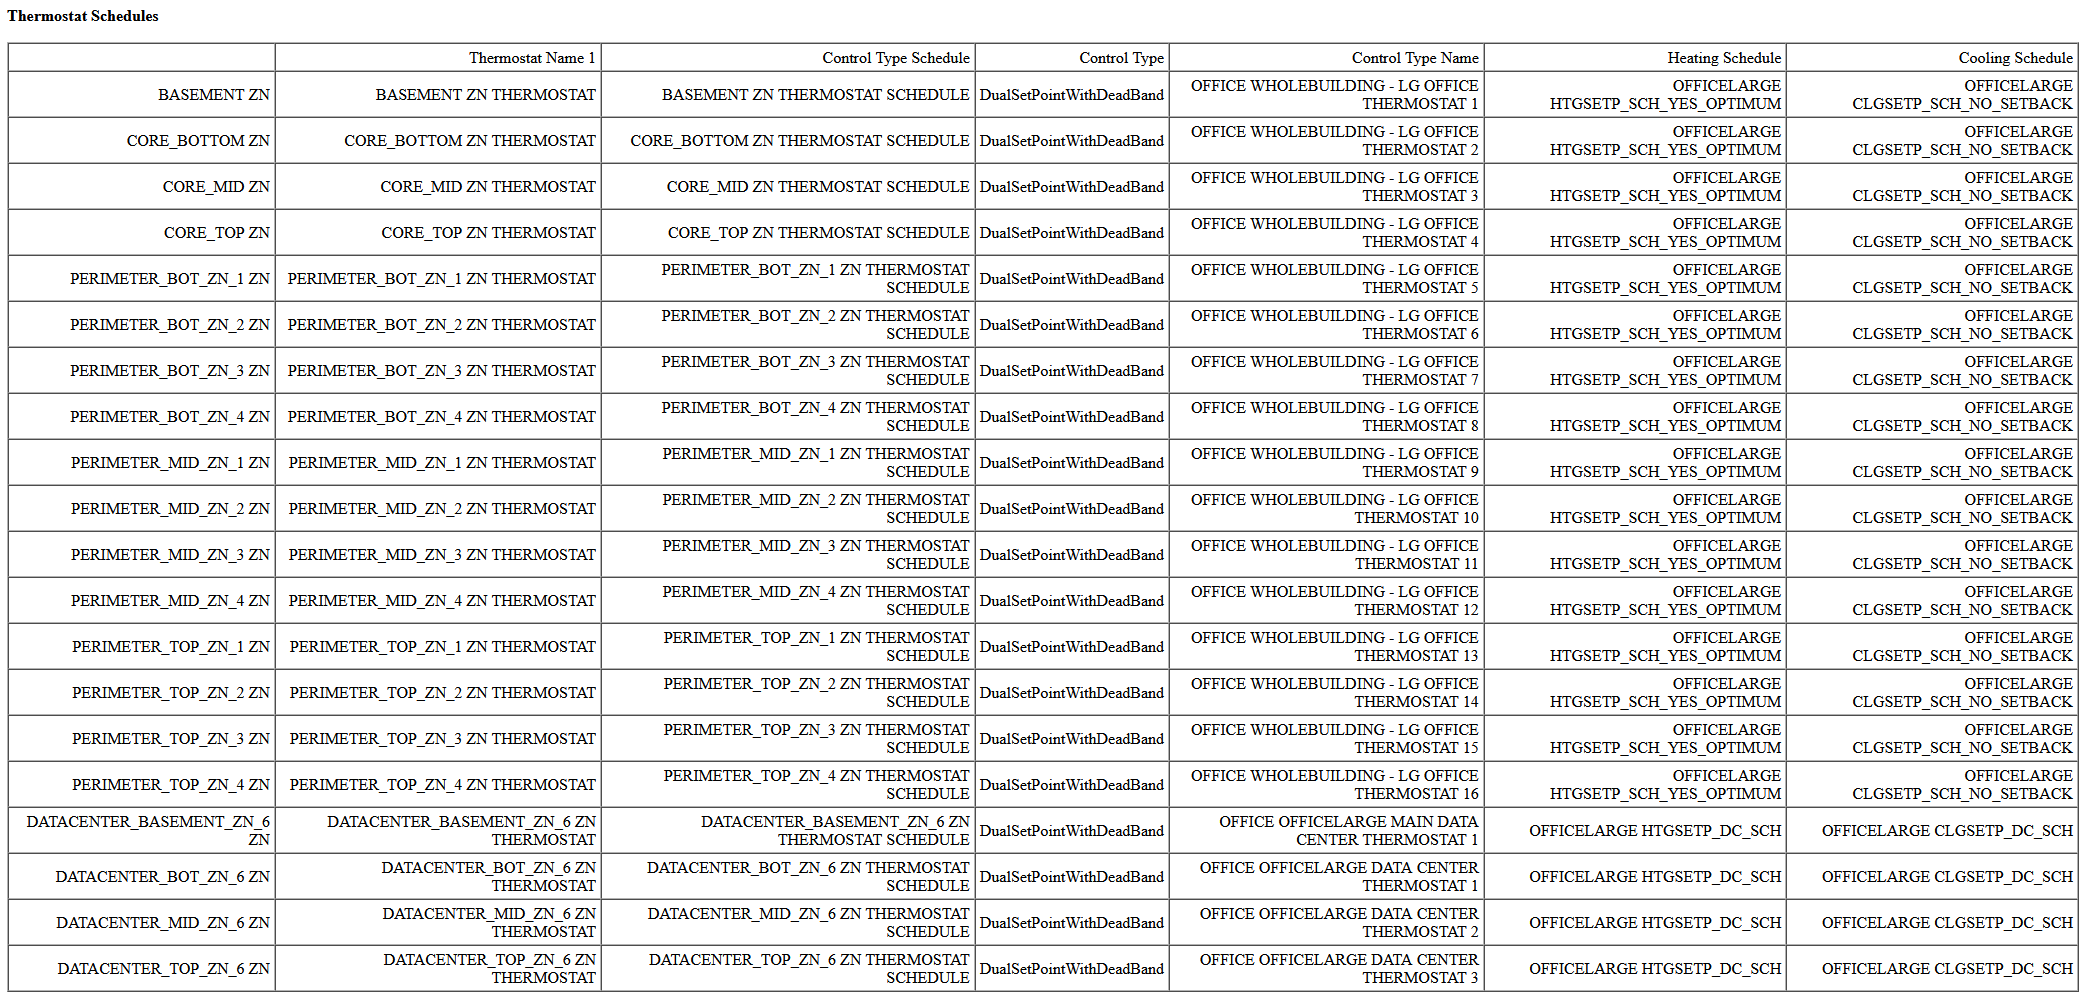
\includegraphics{media/thermostat-schedule-table-example.PNG}
\caption{}
\end{figure}


\subsection{HVAC Topology}\label{hvac-topology}

The HVAC Topology report provides information about the arrangement of HVAC components in the supply and demand side of the airloop, zone equipment, and plant loop. Each row shows the additional component, sub-component, or sub-sub-component being added to the arrangement. 


Air Loop Supply Side Component Arrangement

The columns for this report are shown below as a list:

\begin{itemize}
\item
  Airloop Name
\item
  Upstream Splitter or Mixer Name
\item
  Branch Name
\item
  Component Type
\item
  Component Name
\item
  Sub-Component Type
\item
  Sub-Component Name
\item
  Sub-Sub-Component Type
\item
  Sub-Sub-Component Name
\item
  Downstream Splitter or Mixer Name
\end{itemize}

An example of the report is shown here

\begin{figure}[h!]
\centering
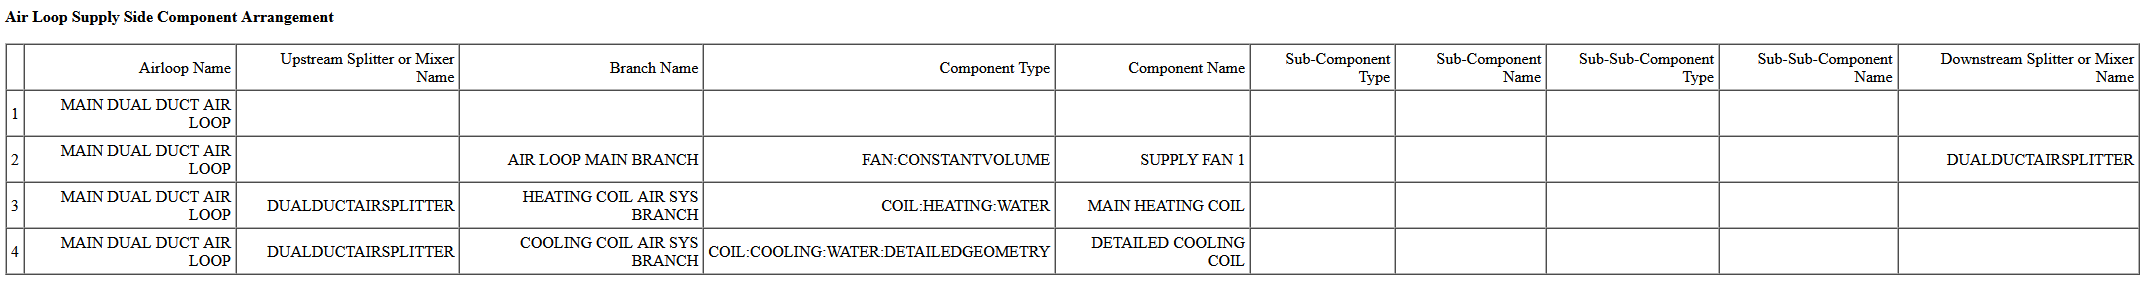
\includegraphics{media/air-supply-side-table-example.PNG}
\caption{}
\end{figure}


Air Loop Demand Side Component Arrangement

The columns for this report are shown below as a list:

\begin{itemize}
\item
  Airloop Name
\item
  Supply Branch Name
\item
  Supply Branch Type
\item
  Supply Path Component Type
\item
  Supply Path Component Name
\item
  Zone Name
\item
  Terminal Unit Type
\item
  Terminal Unit Name
\item
  Return Path Component Type
\item
  Return Path Component Name
\end{itemize}

An example of the report is shown here

\begin{figure}[h!]
\centering
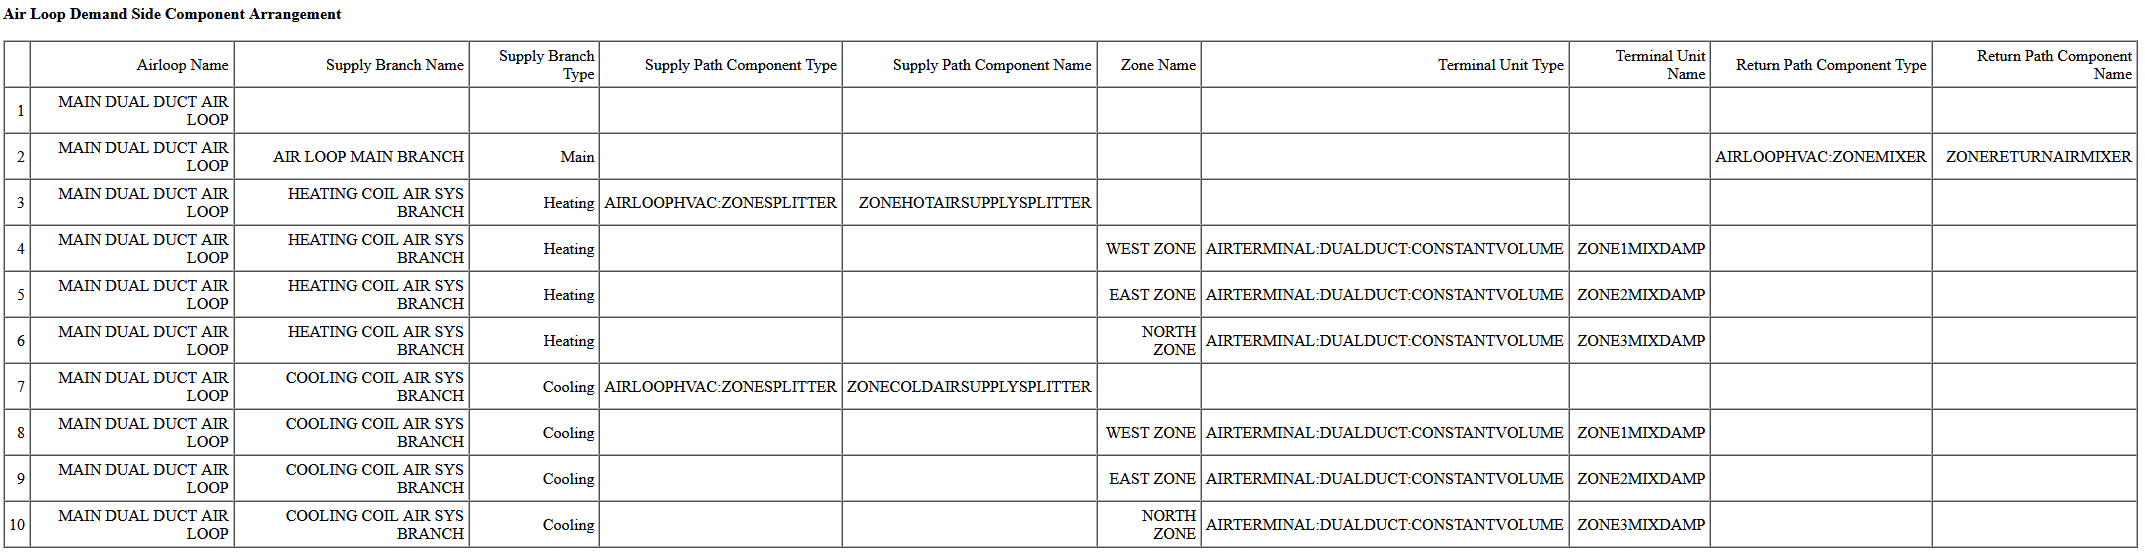
\includegraphics{media/air-demand-side-table-example.PNG}
\caption{}
\end{figure}


Zone Equipment Component Arrangement

The columns for this report are shown below as a list:

\begin{itemize}
\item
  Zone Name
\item
  Component Type
\item
  Component Name
\item
  Sub-Component Type
\item
  Sub-Component Name
\item
  Sub-Sub-Component Type
\item
  Sub-Sub-Component Name
\end{itemize}

An example of the report is shown here

\begin{figure}[h!]
\centering
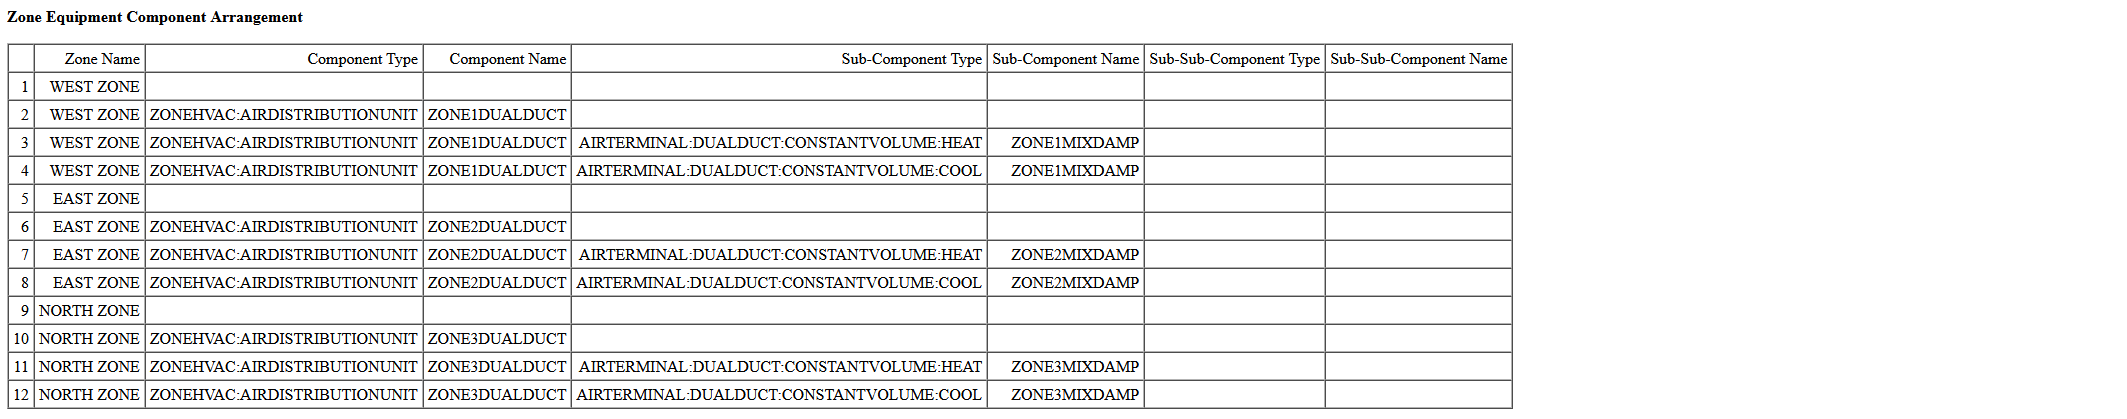
\includegraphics{media/zone-equipment-table-example.png}
\caption{}
\end{figure}


Plant Loop Component Arrangement

The columns for this report are shown below as a list:

\begin{itemize}
\item
  Loop Type
\item
  Loop Name
\item
  Side
\item
  Splitter/Mixer Name
\item
  Branch Name
\item
  Component Type
\item
  Component Name
\end{itemize}

An example of the report is shown here

\begin{figure}[h!]
\centering
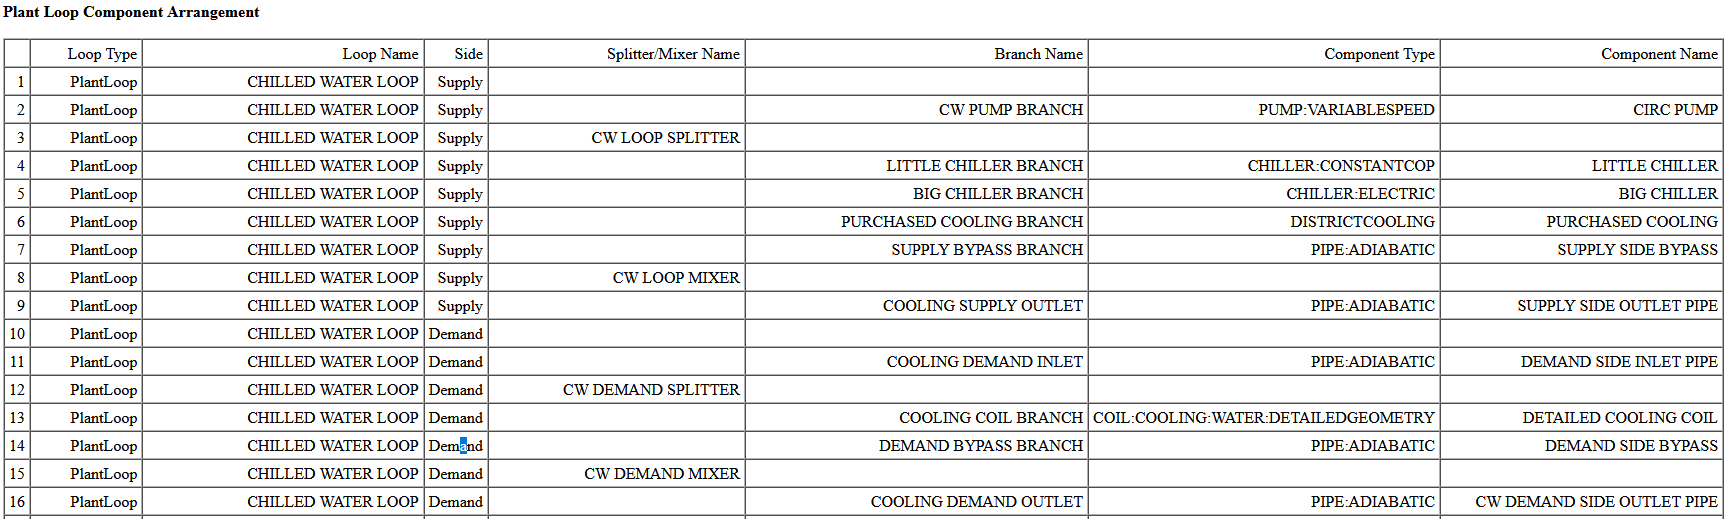
\includegraphics{media/plant-loop-table-example.png}
\caption{}
\end{figure}

\subsection{Component Sizing Summary}\label{component-sizing-summary}

The Component Sizing Summary report includes details on many of the HVAC components in the simulation. For each of the components, one or more parameters are shown. Directly following is an example of the report. The key used to obtain this report is ComponentSizingSummary.

Report: Component Sizing Summary

For: Entire Facility

Timestamp: 2007-10-17 08:54:27

SINGLE DUCT:VAV:REHEAT

\begin{longtable}[c]{>{\raggedright}p{1.52in}>{\raggedright}p{2.24in}>{\raggedright}p{2.24in}}
\toprule 
~ & Maximum air flow rate [m3/s] & Max Reheat Water Flow [m3/s] \tabularnewline
\midrule
\endfirsthead

\toprule 
~ & Maximum air flow rate [m3/s] & Max Reheat Water Flow [m3/s] \tabularnewline
\midrule
\endhead

SPACE1-1 VAV REHEAT & 0.226630 & 0.000059 \tabularnewline
SPACE2-1 VAV REHEAT & 0.176548 & 0.000046 \tabularnewline
SPACE3-1 VAV REHEAT & 0.209331 & 0.000054 \tabularnewline
SPACE4-1 VAV REHEAT & 0.222526 & 0.000058 \tabularnewline
SPACE5-1 VAV REHEAT & 0.221695 & 0.000057 \tabularnewline
\bottomrule
\end{longtable}

COIL:Water:SimpleHeating

\begin{longtable}[c]{>{\raggedright}p{1.5in}>{\raggedright}p{1.5in}>{\raggedright}p{1.5in}>{\raggedright}p{1.5in}}
\toprule 
~ & Max Water Flow Rate of Coil [m3/s] & Design Coil Load [W] & UA of the Coil [W/delK] \tabularnewline
\midrule
\endfirsthead

\toprule 
~ & Max Water Flow Rate of Coil [m3/s] & Design Coil Load [W] & UA of the Coil [W/delK] \tabularnewline
\midrule
\endhead

SPACE1-1 ZONE COIL & 0.000059 & 2698.50 & 66.13 \tabularnewline
SPACE2-1 ZONE COIL & 0.000046 & 2102.17 & 51.51 \tabularnewline
SPACE3-1 ZONE COIL & 0.000054 & 2492.52 & 61.08 \tabularnewline
SPACE4-1 ZONE COIL & 0.000058 & 2649.63 & 64.93 \tabularnewline
SPACE5-1 ZONE COIL & 0.000057 & 2639.74 & 64.69 \tabularnewline
OA HEATING COIL 1 & 0.000148 & 6812.27 & 84.72 \tabularnewline
MAIN HEATING COIL 1 & 0.000075 & 3458.59 & 55.80 \tabularnewline
\bottomrule
\end{longtable}

BRANCH

\begin{longtable}[c]{@{}ll@{}}
\toprule 
~ & Maximum Branch Flow Rate [m3/s] \tabularnewline
\midrule
\endfirsthead

\toprule 
~ & Maximum Branch Flow Rate [m3/s] \tabularnewline
\midrule
\endhead

VAV SYS 1 MAIN BRANCH & 1.06 \tabularnewline
\bottomrule
\end{longtable}

AIR PRIMARY LOOP

\begin{longtable}[c]{@{}ll@{}}
\toprule 
~ & Primary air design volumetric flow rate [m3/s] \tabularnewline
\midrule
\endfirsthead

\toprule 
~ & Primary air design volumetric flow rate [m3/s] \tabularnewline
\midrule
\endhead

VAV SYS 1 & 1.06 \tabularnewline
\bottomrule
\end{longtable}

CONTROLLER:OUTSIDE AIR

\begin{longtable}[c]{>{\raggedright}p{1.5in}>{\raggedright}p{2.25in}>{\raggedright}p{2.25in}}
\toprule 
~ & maximum outside air flow rate [m3/s] & minimum outside air flow rate [m3/s] \tabularnewline
\midrule
\endfirsthead

\toprule 
~ & maximum outside air flow rate [m3/s] & minimum outside air flow rate [m3/s] \tabularnewline
\midrule
\endhead

OA CONTROLLER 1 & 1.06 & 0.264118 \tabularnewline
\bottomrule
\end{longtable}

COIL:Water:Cooling

\begin{longtable}[c]{>{\raggedright}p{0.75in}>{\raggedright}p{0.75in}>{\raggedright}p{0.75in}>{\raggedright}p{0.75in}>{\raggedright}p{0.75in}>{\raggedright}p{0.75in}>{\raggedright}p{0.75in}>{\raggedright}p{0.75in}}
\toprule 
~ & Max Water Flow Rate of Coil [m3/s] & Max Air Flow Rate of Coil [m3/s] & Design Air Inlet Temperature [C] & Design Air Outlet Temperature [C] & Design Water Inlet Temperature [C] & Design Air Inlet Humidity Ratio & Design Air Outlet Humidity Ratio \tabularnewline
\midrule
\endfirsthead

\toprule 
~ & Max Water Flow Rate of Coil [m3/s] & Max Air Flow Rate of Coil [m3/s] & Design Air Inlet Temperature [C] & Design Air Outlet Temperature [C] & Design Water Inlet Temperature [C] & Design Air Inlet Humidity Ratio & Design Air Outlet Humidity Ratio \tabularnewline
\midrule
\endhead

OA COOLING COIL 1 & 0.001145 & 0.264118 & 30.01 & 11.00 & 7.00 & 0.014595 & 0.008000 \tabularnewline
MAIN COOLING COIL 1 & 0.000916 & 1.06 & 21.55 & 12.80 & 7.00 & 0.009333 & 0.008000 \tabularnewline
\bottomrule
\end{longtable}

FAN:SIMPLE:VARIABLEVOLUME

\begin{longtable}[c]{@{}lll@{}}
\toprule 
~ & Max Flow Rate [m3/s] & Min Flow Rate [m3/s] \tabularnewline
\midrule
\endfirsthead

\toprule 
~ & Max Flow Rate [m3/s] & Min Flow Rate [m3/s] \tabularnewline
\midrule
\endhead

SUPPLY FAN 1 & 1.06 & 0.353263 \tabularnewline
\bottomrule
\end{longtable}

CONTROLLER:SIMPLE

\begin{longtable}[c]{@{}ll@{}}
\toprule 
~ & Max Actuated Flow [m3/s] \tabularnewline
\midrule
\endfirsthead

\toprule 
~ & Max Actuated Flow [m3/s] \tabularnewline
\midrule
\endhead

OA CC CONTROLLER 1 & 0.001145 \tabularnewline
OA HC CONTROLLER 1 & 0.000148 \tabularnewline
CENTRAL COOLING COIL CONTROLLER 1 & 0.000916 \tabularnewline
CENTRAL HEATING COIL CONTROLLER 1 & 0.000075 \tabularnewline
\bottomrule
\end{longtable}

PLANT LOOP

\begin{longtable}[c]{>{\raggedright}p{1.5in}>{\raggedright}p{2.62in}>{\raggedright}p{1.87in}}
\toprule 
~ & Maximum Loop Volumetric Flow Rate [m3/s] & Volume of the plant loop [m3] \tabularnewline
\midrule
\endfirsthead

\toprule 
~ & Maximum Loop Volumetric Flow Rate [m3/s] & Volume of the plant loop [m3] \tabularnewline
\midrule
\endhead

HOT WATER LOOP & 0.000497 & 0.559158 \tabularnewline
CHILLED WATER LOOP & 0.002061 & 2.32 \tabularnewline
\bottomrule
\end{longtable}

BOILER:SIMPLE

\begin{longtable}[c]{>{\raggedright}p{1.5in}>{\raggedright}p{1.56in}>{\raggedright}p{2.93in}}
\toprule 
~ & Nominal Capacity [W] & Design Boiler Water Flow Rate [m3/s] \tabularnewline
\midrule
\endfirsthead

\toprule 
~ & Nominal Capacity [W] & Design Boiler Water Flow Rate [m3/s] \tabularnewline
\midrule
\endhead

CENTRAL BOILER & 22853.43 & 0.000497 \tabularnewline
\bottomrule
\end{longtable}

CHILLER:ELECTRIC

\begin{longtable}[c]{>{\raggedright}p{1.5in}>{\raggedright}p{1.5in}>{\raggedright}p{3.0in}}
\toprule 
~ & Nominal Capacity [W] & Design Evaporator Volumetric Water Flow Rate [m3/s] \tabularnewline
\midrule
\endfirsthead

\toprule 
~ & Nominal Capacity [W] & Design Evaporator Volumetric Water Flow Rate [m3/s] \tabularnewline
\midrule
\endhead

CENTRAL CHILLER & 34468.25 & 0.002061 \tabularnewline
\bottomrule
\end{longtable}

PUMP:VARIABLE SPEED

\begin{longtable}[c]{>{\raggedright}p{1.5in}>{\raggedright}p{2.5in}>{\raggedright}p{2.0in}}
\toprule 
~ & Rated Volumetric Flow Rate [m3/s] & Rated Power Consumption [W] \tabularnewline
\midrule
\endfirsthead

\toprule 
~ & Rated Volumetric Flow Rate [m3/s] & Rated Power Consumption [W] \tabularnewline
\midrule
\endhead

HW CIRC PUMP & 0.000497 & 126.98 \tabularnewline
CW CIRC PUMP & 0.002061 & 526.69 \tabularnewline
\bottomrule
\end{longtable}

\subsection{Outdoor Air Summary}\label{outdoor-air-summary}

The Outdoor Air Summary provides information for each zone on the average and minimum ventilation provided.

The reports described so far in this section are displayed when specified in the Output:Table:SummaryReports object. They are either on or off and are not customizable. The next few types of tabular reports are customizable. You can specify the report variables being used in each one.

Directly following is an example of the report. The key used to obtain this report is OutdoorAirSummary.

Report: Outdoor Air Summary

For: Entire Facility

Timestamp: 2007-10-17 08:54:27

Average Outside Air During Occupied Hours

\begin{longtable}[c]{>{\raggedright}p{0.85in}>{\raggedright}p{0.85in}>{\raggedright}p{0.85in}>{\raggedright}p{0.85in}>{\raggedright}p{0.85in}>{\raggedright}p{0.85in}>{\raggedright}p{0.85in}}
\toprule 
~ & Average Number of Occupants & Nominal Number of Occupants & Zone Volume (m3) & Mechanical Ventilation (ach) & Infiltration (ach) & Simple Ventilation (ach) \tabularnewline
\midrule
\endfirsthead

\toprule 
~ & Average Number of Occupants & Nominal Number of Occupants & Zone Volume (m3) & Mechanical Ventilation (ach) & Infiltration (ach) & Simple Ventilation (ach) \tabularnewline
\midrule
\endhead

SPACE1-1 & 9.50 & 11.00 & 239.25 & 0.365 & 0.050 & 0.000 \tabularnewline
SPACE2-1 & 4.32 & 5.00 & 103.31 & 0.630 & 0.051 & 0.000 \tabularnewline
SPACE3-1 & 9.50 & 11.00 & 239.25 & 0.338 & 0.050 & 0.000 \tabularnewline
SPACE4-1 & 4.32 & 5.00 & 103.31 & 0.708 & 0.051 & 0.000 \tabularnewline
SPACE5-1 & 17.27 & 20.00 & 447.68 & 0.214 & 0.052 & 0.000 \tabularnewline
\bottomrule
\end{longtable}

Minimum Outside Air During Occupied Hours

\begin{longtable}[c]{>{\raggedright}p{0.85in}>{\raggedright}p{0.85in}>{\raggedright}p{0.85in}>{\raggedright}p{0.85in}>{\raggedright}p{0.85in}>{\raggedright}p{0.85in}>{\raggedright}p{0.85in}}
\toprule 
~ & Average Number of Occupants & Nominal Number of Occupants & Zone Volume (m3) & Mechanical Ventilation (ach) & Infiltration (ach) & Simple Ventilation (ach) \tabularnewline
\midrule
\endfirsthead

\toprule 
~ & Average Number of Occupants & Nominal Number of Occupants & Zone Volume (m3) & Mechanical Ventilation (ach) & Infiltration (ach) & Simple Ventilation (ach) \tabularnewline
\midrule
\endhead

SPACE1-1 & 9.50 & 11.00 & 239.25 & 0.000 & 0.000 & 0.000 \tabularnewline
SPACE2-1 & 4.32 & 5.00 & 103.31 & 0.000 & 0.000 & 0.000 \tabularnewline
SPACE3-1 & 9.50 & 11.00 & 239.25 & 0.000 & 0.000 & 0.000 \tabularnewline
SPACE4-1 & 4.32 & 5.00 & 103.31 & 0.000 & 0.000 & 0.000 \tabularnewline
SPACE5-1 & 17.27 & 20.00 & 447.68 & 0.000 & 0.000 & 0.000 \tabularnewline
\bottomrule
\end{longtable}

\subsection{Outdoor Air Details}\label{outdoor-air-details}

The Outdoor Air Details report provides detailed information on outdoor air flow for each zone and air loop. This report may be specified in the  Output:Table:SummaryReports object with the key OutdoorAirDetails. It is also produced for any AllSummary* key. Each subtable and column are described below.

\subsubsection{Mechanical Ventilation Parameters by Zone}\label{mechanical-ventilation-parameters-by-zone}
\begin{description}
  \item[AirLoop Name] The name(s) of air loop(s) serving this zone,if any.
  \item[Average Number of Occupants] Average number of occupants during occupied times (occupants > 0) for the simulation period.
  \item[Nominal Number of Occupants] Total number of people for all People objects in this zone (ignoring schedules).
  \item[Zone Volume] The zone volume in \si{\volume}.
  \item[Zone Area] The zone floor area in \si{\area}.
  \item[Design Zone Outdoor Airflow - \(V_{oz}\)] The design outdoor air flow rate specified in the DesignSpecification:OutdoorAir object for this zone in \si{\volumeFlowRate}. This is the outdoor air flow rate used for sizing without any schedule modifier.
  \item[Minimum Dynamic Target Ventilation - \(V_{oz-dyn-min}\)] The minimum outdoor air flow rate specified in the DesignSpecification:OutdoorAir object for this zone in \si{\volumeFlowRate}. This is the outdoor air flow rate for the minimum number of occupants without any schedule modifier.
\end{description}

\subsubsection{Total Outdoor Air by Zone}\label{total-outdoor-air-by-zone}
\begin{description}
  \item[Mechanical Ventilation] The total outdoor air delivered to this zone by mechanical ventilation (HVAC systems) in \si{\volume} (Output:Variable Zone Mechanical Ventilation Standard Density Volume Flow Rate).

  \item[Natural Ventilation] The total outdoor air delivered to this zone by natural ventilation (ZoneVentilation:* or AirflowNetwork) in \si{\volume}.

  \item[Total Ventilation] The sum of Mechanical and Natural Ventilation in \si{\volume}.

  \item[Infiltration] The total outdoor air delivered to this zone by infiltration (ZoneInfiltration:* or AirflowNetwork) in \si{\volume} (Output:Variable Zone Infiltration Standard Density Volume Flow Rate).

  \item[Total Ventilation and Infiltration] The sum of Mechanical and Natural Ventilation and Infiltration in \si{\volume}.

  \item[Dynamic Target Ventilation - \(V_{oz-dyn}\)] The total dynamic outdoor air flow rate specified in the DesignSpecification:OutdoorAir object for this zone in \si{\volumeFlowRate}. This is the zone target ventilation flow rate \(V_{oz-dyn}\) at standard density at the current timestep including any schedule modifier (Output:Variable Zone Target Voz Ventilation Flow Rate).

  \item[Time Below \(V_{oz-dyn}\)] The time in hours that the Total Ventilation rate (mechanical ventilation plus natural ventilation) is more than 1\% below the Dynamic Target Ventilation - \(V_{oz-dyn}\) flow rate (Output:Variable Zone Ventilation Below Target Voz Time).

  \item[Time At \(V_{oz-dyn}\)] The time in hours that the Total Ventilation rate (mechanical ventilation plus natural ventilation) is within 1\% of the Dynamic Target Ventilation - \(V_{oz-dyn}\) flow rate (Output:Variable Zone Ventilation At Target Voz Time).

  \item[Time Above \(V_{oz-dyn}\)] The time in hours that the Total Ventilation rate (mechanical ventilation plus natural ventilation) is more than 1\% above the Dynamic Target Ventilation - \(V_{oz-dyn}\) flow rate (Output:Variable Zone Ventilation Above Target Voz Time).

  \item[Time Above Zero When Unoccupied] The time in hours that the Total Ventilation rate (mechanical ventilation plus natural ventilation) is greater than zero when the zone is unoccupied (Output:Variable Zone Ventilation When Unoccupied Time).
\end{description}

\subsubsection{Average Outdoor Air During Occupancy by Zone - Flow Rates}\label{average-outdoor-air-during-occupancy-by-zone-flow-rates}
This subtable is the same as Total Outdoor Air by Zone except that it reports average flow rates in \si{\volumeFlowRate} and status times in hours for occupied periods only.

\subsubsection{Total Outdoor Air by AirLoop}\label{total-outdoor-air-by-airloop}
\begin{description}
  \item[Mechanical Ventilation] The total outdoor air delivered to the zones on this air loop by only this air loop in \si{\volume} (Output:Variable Air System Mechanical Ventilation Flow Rate).

  \item[Natural Ventilation] The total outdoor air delivered to the zones on this air loop by natural ventilation (ZoneVentilation:* or AirflowNetwork) in \si{\volume} (Output:Variable Air System Natural Ventilation Flow Rate). If any zone terminal unit has a DesignSpecification:AirTerminal:Sizing object then the natural ventilation rate for that zone is scaled by the Fraction of Minimum Outdoor Air Flow value.

  \item[Total Ventilation] The sum of Mechanical and Natural Ventilation in \si{\volume}.

  \item[Sum Zone Dynamic Target Ventilation - \(V_{oz-dyn}\)] The total dynamic outdoor air flow rate specified in the DesignSpecification:OutdoorAir object for the zones on this air loop in \si{\volumeFlowRate}. This is the sum of the zone target ventilation flow rates \(V_{oz-dyn}\) at standard density at the current timestep including any schedule modifier (Output:Variable Air System Target Voz Ventilation Flow Rate). If any zone terminal unit has a DesignSpecification:AirTerminal:Sizing object then the target ventilation rate for that zone is scaled by the Fraction of Minimum Outdoor Air Flow value.

  \item[Time Below \(V_{oz-dyn}\)] The time in hours that the Total Ventilation rate (mechanical ventilation plus natural ventilation) is more than 1\% below the Sum Zone Dynamic Target Ventilation - \(V_{oz-dyn}\) flow rate (Output:Variable Air System Ventilation Below Target Voz Time).

  \item[Time At \(V_{oz-dyn}\)] The time in hours that the Total Ventilation rate (mechanical ventilation plus natural ventilation) is within 1\% of the Sum Zone Dynamic Target Ventilation - \(V_{oz-dyn}\) flow rate (Output:Variable Air System Ventilation At Target Voz Time).

  \item[Time Above \(V_{oz-dyn}\)] The time in hours that the Total Ventilation rate (mechanical ventilation plus natural ventilation) is more than 1\% above the Sum Zone Dynamic Target Ventilation - \(V_{oz-dyn}\) flow rate (Output:Variable Air System Ventilation Above Target Voz Time).

  \item[Time Above Zero When Unoccupied] The time in hours that the Total Ventilation rate (mechanical ventilation plus natural ventilation) is greater than zero when the all zones on this air loop are unoccupied (Output:Variable Air System Ventilation When Unoccupied Time).
\end{description}

\subsubsection{Average Outdoor Air During Occupancy by AirLoop}\label{average-outdoor-air-during-occupancy-by-airloop}
This subtable is the same as Total Outdoor Air by AirLoop except that it reports average flow rates in \si{\volumeFlowRate} and status times in hours when any zone on this air loop is occupied.

\subsubsection{Outdoor Air Controller Limiting Factors by AirLoop}\label{outdoor-air-controller-limiting-factors-by-airloop}
  Times in hours that the outdoor air flow rate for this airloop is set by one of the following limiting factors (Output:Variable Air System Outdoor Air Limiting Factor).
\begin{description}
  \item[No Limiting Factor] None of the other limiting factors is active.
  \item[Limits and Scheduled Limits] Fixed limits such as Controller:OutdoorAir Minimum Outdoor Air Flow Rate, Maximum Outdoor Air Flow Rate, Minimum Fraction of Outdoor Air Schedule Name, Maximum Fraction of Outdoor Air Schedule Name.
  \item[Economizer] Economizer is active and sets the flow greater than the minimum outdoor air fraction.
  \item[Exhaust Flow] Outdoor air flow rate equals the total zone exhaust flow rate.
  \item[Mixed Air Flow] Outdoor air flow rate is limited by the current mixed air flow rate.
  \item[High Humidity] Controller:OutdoorAir High Humidity Control.
  \item[Demand Controlled Ventilation] Controller:MechanicalVentilation requested more than the minimum outdoor air fraction.
  \item[Night Ventilation] AvailabilityManager:NightVentilation is active.
  \item[Demand Limiting] DemandManager:Ventilation has reduced the outdoor air flow rate.
  \item[Energy Management System] An EnergyManagementSystem:Actuator has overridden the outdoor air flow rate.
\end{description}

\subsubsection{Average Outdoor Air for Limiting Factors During Occupancy}\label{average-outdoor-air-for-limiting-factors-during-occupancy}
This subtable is the same as Outdoor Air Controller Limiting Factors by AirLoop except that it reports average flow rates in \si{\volumeFlowRate} at each limiting factor for occupied periods only.


\subsection{Climatic Data Summary}\label{climatic-data-summary}

The Climatic Data Summary provides some statistics from the .STAT file concerning the selected weather. The Stat file must be available (it is included with all the weather files on the EnergyPlus website) for the report to be fully produced. Directly following is an example of the report. The key used to obtain this report is ClimaticDataSummary.

Report: Climatic Data Summary

For: Entire Facility

Timestamp: 2009-02-10 13:27:45

SizingPeriod:DesignDay

\begin{longtable}[c]{>{\raggedright}p{0.85in}>{\raggedright}p{0.85in}>{\raggedright}p{0.85in}>{\raggedright}p{0.85in}>{\raggedright}p{0.85in}>{\raggedright}p{0.85in}>{\raggedright}p{0.85in}}
\toprule 
~ & Maximum Dry Bulb (C) & Daily Temperature Range (C) & Humidity Value & Humidity Type & Wind Speed (m/s) & Wind Direction \tabularnewline
\midrule
\endfirsthead

\toprule 
~ & Maximum Dry Bulb (C) & Daily Temperature Range (C) & Humidity Value & Humidity Type & Wind Speed (m/s) & Wind Direction \tabularnewline
\midrule
\endhead

CHICAGO\-\_IL\-\_USA ANNUAL HEATING 99\% DESIGN CONDITIONS DB & -17.30 & 0.00 & -17.30 & WETBULB & 4.90 & 270.00 \tabularnewline
CHICAGO\-\_IL\-\_USA ANNUAL COOLING 1\% DESIGN CONDITIONS DB/MCWB & 31.50 & 10.70 & 23.00 & WETBULB & 5.30 & 230.00 \tabularnewline
\bottomrule
\end{longtable}

Weather Statistics File

\begin{longtable}[c]{>{\raggedright}p{2.02in}>{\raggedright}p{3.96in}}
\toprule 
~ & Value \tabularnewline
\midrule
\endfirsthead

\toprule 
~ & Value \tabularnewline
\midrule
\endhead

Reference & USA\_Chicago-OHare\_TMY2 \tabularnewline
Site:Location & Chicago IL USA \tabularnewline
Latitude & N 41° 58' \tabularnewline
Longitude & W 87° 54' \tabularnewline
Time Zone & GMT -6.0 Hours \tabularnewline
Elevation & 190m above sea level \tabularnewline
Standard Pressure at Elevation & 99063Pa \tabularnewline
Data Source & Release Test \tabularnewline
WMO Station & 725300 \tabularnewline
Design Conditions & Climate Design Data 2005 ASHRAE Handbook \tabularnewline
Heating Design Temperature 99.6\% (C) & -20.6 \tabularnewline
Heating Design Temperature 99\% (C) & -17.3 \tabularnewline
Cooling Design Temperature 0.4\% (C) & 33.2 \tabularnewline
Cooling Design Temperature 1\% (C) & 31.5 \tabularnewline
Cooling Design Temperature 2\% (C) & 29.9 \tabularnewline
Maximum Dry Bulb Temperature (C) & 35.6° \tabularnewline
Maximum Dry Bulb Occurs on & Jul 9 \tabularnewline
Minimum Dry Bulb Temperature (C) & -22.8° \tabularnewline
Minimum Dry Bulb Occurs on & Jan 7 \tabularnewline
Maximum Dew Point Temperature (C) & 25.6 \tabularnewline
Maximum Dew Point Occurs on & Aug 4 \tabularnewline
Minimum Dew Point Temperature (C) & -28.9 \tabularnewline
Minimum Dew Point Occurs on & Dec 31 \tabularnewline
Heating Degree-Days (base 10°C) & 1745 \tabularnewline
Cooling Degree-Days (base 18°C) & 464 \tabularnewline
Köppen Classification & Dfa \tabularnewline
Köppen Description & Humid continental (hot summer, cold winter, no dry season, lat. 30-60°N) \tabularnewline
Köppen Recommendation & Unbearably humid periods in summer, but passive cooling is possible \tabularnewline
ASHRAE Climate Zone & 5A \tabularnewline
ASHRAE Description & Cool-Humid \tabularnewline
\bottomrule
\end{longtable}

\subsection{Object Count Summary}\label{object-count-summary}

The object count summary report provides the count on the number of specific objects in the file. Directly following is an example of the report. The key used to obtain this report is ObjectCountSummary.

Report: Object Count Summary

For: Entire Facility

Timestamp: 2009-02-10 12:39:35

Surfaces by Class

\begin{longtable}[c]{@{}lll@{}}
\toprule 
~ & Total & Outdoors \tabularnewline
\midrule
\endfirsthead

\toprule 
~ & Total & Outdoors \tabularnewline
\midrule
\endhead

Wall & 24 & 8 \tabularnewline
Floor & 10 & 5 \tabularnewline
Roof & 6 & 1 \tabularnewline
Internal Mass & 0 & 0 \tabularnewline
Building Detached Shading & 0 & 0 \tabularnewline
Fixed Detached Shading & 0 & 0 \tabularnewline
Window & 6 & 6 \tabularnewline
Door & 0 & 0 \tabularnewline
Glass Door & 0 & 0 \tabularnewline
Shading & 4 & 4 \tabularnewline
Overhang & 0 & 0 \tabularnewline
Fin & 0 & 0 \tabularnewline
Tubular Daylighting Device Dome & 0 & 0 \tabularnewline
Tubular Daylighting Device Diffuser & 0 & 0 \tabularnewline
\bottomrule
\end{longtable}

HVAC

\begin{longtable}[c]{@{}ll@{}}
\toprule 
~ & Count \tabularnewline
\midrule
\endfirsthead

\toprule 
~ & Count \tabularnewline
\midrule
\endhead

HVAC Air Loops & 1 \tabularnewline
Conditioned Zones & 6 \tabularnewline
Unconditioned Zones & 0 \tabularnewline
Supply Plenums & 0 \tabularnewline
Return Plenums & 1 \tabularnewline
\bottomrule
\end{longtable}

\subsection{Component Cost Economics Summary}\label{component-cost-economics-summary}

The Component Cost Economics Summary provides the construction cost estimate summary for the project. The costs are broken into eight categories and the reference building costs are provided as a comparison. A second table is also produced that provides line item details with one line for every line item object. Directly following is an example of this report.

Report: Component Cost Economics Summary

For: Entire Facility

Timestamp: 2016-01-12 15:47:39

Construction Cost Estimate Summary

\begin{longtable}[c]{>{\raggedright}p{1.5in}>{\raggedright}p{1.5in}>{\raggedright}p{1.5in}>{\raggedright}p{1.5in}}
\toprule 
 & Reference Bldg. & Current Bldg. Model & Difference \tabularnewline
\midrule
\endfirsthead

\toprule 
 & Reference Bldg. & Current Bldg. Model & Difference \tabularnewline
\midrule
\endhead

Line Item SubTotal (\$) & 665082.04 & 719946.72 & 54864.68 \tabularnewline
Misc. Costs (\$) & 928979.09 & 928979.09 & 0 \tabularnewline
Regional Adjustment (\$) & 216792.31 & 224253.91 & 7461.6 \tabularnewline
Design Fee (\$) & 108651.21 & 149854.38 & 41203.17 \tabularnewline
Contractor Fee (\$) & 126759.74 & 131122.58 & 4362.84 \tabularnewline
Contingency (\$) & 181085.34 & 187317.97 & 6232.63 \tabularnewline
Permits, Bonds, Insurance (\$) & 0 & 0 & 0 \tabularnewline
Commissioning (\$) & 9054.27 & 18731.8 & 9677.53 \tabularnewline
Cost Estimate Total (\$) & 2236404 & 2360206.45 & 123802.44 \tabularnewline
Cost Per Conditioned Building Area (\$/m2) & 1203.69 & 1270.32 & 66.63 \tabularnewline
\bottomrule
\end{longtable}

Cost Line Item Details

\begin{longtable}[c]{>{\raggedright}p{0.85in}>{\raggedright}p{0.85in}>{\raggedright}p{0.85in}>{\raggedright}p{0.85in}>{\raggedright}p{0.85in}>{\raggedright}p{0.85in}>{\raggedright}p{0.85in}}
\toprule 
 & Line No. & Item Name & Quantity. & Units & \$ per Qty. & SubTotal \$ \tabularnewline
\midrule
\endfirsthead

\toprule 
 & Line No. & Item Name & Quantity. & Units & \$ per Qty. & SubTotal \$ \tabularnewline
\midrule
\endhead

-- & 1 & EXTERIOR WALLS & 627.57 & m2 & 168.64 & 105832.65 \tabularnewline
-- & 2 & INTERIOR WALLS & 854.18 & m2 & 31.16 & 26616.23 \tabularnewline
-- & 3 & ROOF & 1857.96 & m2 & 104.69 & 194509.64 \tabularnewline
-- & 4 & GROUND FLR SLAB & 1857.96 & m2 & 56.06 & 104157.14 \tabularnewline
-- & 5 & ACOUSTICAL DROP CEILINGS & 1857.96 & m2 & 23.79 & 44200.83 \tabularnewline
-- & 6 & QUAD HIGH SHGC SUPERWINDOWS & 226.22 & m2 & 687.84 & 155604.96 \tabularnewline
-- & 7 & QUAD LOW SHGC SUPERWINDOWS & 42.68 & m2 & 687.84 & 29359.55 \tabularnewline
-- & 8 & CENTRAL CHILLER & 150.49 & kW (tot cool cap.) & 340 & 51165.73 \tabularnewline
-- & 9 & CONTINUOUS AIR BARRIER & 1 & Ea. & 8500 & 8500 \tabularnewline
Line Item SubTotal & -- & -- & -- & -- & -- & 719946.72 \tabularnewline
\bottomrule
\end{longtable}

\subsection{LEED Summary}\label{leed-summary}

The LEED Summary report provides many of the simulation results required for certification of Energy and Atmosphere Credit 1 Optimized Energy Performance according to the LEED Green Building Rating System\textsuperscript{TM}. The report can be produced by specifying LEEDSummary in Output:Table:SummaryReports which is also part of the AllSummary option. Directly following is an example of this report.

Report: LEED Summary

For: Entire Facility

Timestamp: 2013-03-01 15:24:37

Sec1.1A-General Information

\begin{longtable}[c]{>{\raggedright}p{2.21in}>{\raggedright}p{3.78in}}
\toprule 
 & Data \tabularnewline
\midrule
\endfirsthead

\toprule 
 & Data \tabularnewline
\midrule
\endhead

Heating Degree Days & 1748 \tabularnewline
Cooling Degree Days & 506 \tabularnewline
Climate Zone & 5A \tabularnewline
Weather File & Chicago Ohare Intl Ap IL USA TMY3 WMO\#=725300 \tabularnewline
HDD and CDD data source & Weather File Stat \tabularnewline
Total gross floor area [m2] & 927.20 \tabularnewline
Principal Heating Source & Natural Gas \tabularnewline
\bottomrule
\end{longtable}

EAp2-1. Space Usage Type

\begin{longtable}[c]{>{\raggedright}p{1.2in}>{\raggedright}p{1.2in}>{\raggedright}p{1.2in}>{\raggedright}p{1.2in}>{\raggedright}p{1.2in}}
\toprule 
 & Space Area [m2] & Regularly Occupied Area [m2] & Unconditioned Area [m2] & Typical Hours/Week in Operation [hr/wk] \tabularnewline
\midrule
\endfirsthead

\toprule 
 & Space Area [m2] & Regularly Occupied Area [m2] & Unconditioned Area [m2] & Typical Hours/Week in Operation [hr/wk] \tabularnewline
\midrule
\endhead

SPACE1-1 & 99.16 & 99.16 & 0.00 & 55.06 \tabularnewline
SPACE2-1 & 42.73 & 42.73 & 0.00 & 55.06 \tabularnewline
SPACE3-1 & 96.48 & 96.48 & 0.00 & 55.06 \tabularnewline
SPACE4-1 & 42.73 & 42.73 & 0.00 & 55.06 \tabularnewline
SPACE5-1 & 182.49 & 182.49 & 0.00 & 55.06 \tabularnewline
PLENUM-1 & 463.60 & 463.60 & 0.00 & 0.00 \tabularnewline
Totals & 927.20 & 927.20 & 0.00 & ~ \tabularnewline
\bottomrule
\end{longtable}

EAp2-2. Advisory Messages

\begin{longtable}[c]{@{}ll@{}}
\toprule 
 & Data \tabularnewline
\midrule
\endfirsthead

\toprule 
 & Data \tabularnewline
\midrule
\endhead

Number of hours heating loads not met & 0.00 \tabularnewline
Number of hours cooling loads not met & 10.75 \tabularnewline
Number of hours not met & 10.75 \tabularnewline
\bottomrule
\end{longtable}

EAp2-3. Energy Type Summary

\begin{longtable}[c]{>{\raggedright}p{1.2in}>{\raggedright}p{1.2in}>{\raggedright}p{1.2in}>{\raggedright}p{1.2in}>{\raggedright}p{1.2in}}
\toprule 
 & Utility Rate & Virtual Rate [\textbackslash\$/unit energy] & Units of Energy & Units of Demand \tabularnewline
\midrule
\endfirsthead

\toprule 
 & Utility Rate & Virtual Rate [\textbackslash\$/unit energy] & Units of Energy & Units of Demand \tabularnewline
\midrule
\endhead

Electricity & EXAMPLEA EXAMPLEI-SELL & 0.055 & kWh & kW \tabularnewline
Natural Gas & EXAMPLEA-GAS & 0.569 & Therm & Therm/Hr \tabularnewline
Other & ~ & ~ & ~ & ~ \tabularnewline
\bottomrule
\end{longtable}

EAp2-4/5. Performance Rating Method Compliance

\begin{longtable}[c]{>{\raggedright}p{0.85in}>{\raggedright}p{0.85in}>{\raggedright}p{0.85in}>{\raggedright}p{0.85in}>{\raggedright}p{0.85in}>{\raggedright}p{0.85in}>{\raggedright}p{0.85in}}
\toprule 
 & Electric Energy Use [GJ] & Electric Demand [W] & Natural Gas Energy Use [GJ] & Natural Gas Demand [W] & Other Fuel Use [GJ] & Other Fuel Demand [W] \tabularnewline
\midrule
\endfirsthead

\toprule 
 & Electric Energy Use [GJ] & Electric Demand [W] & Natural Gas Energy Use [GJ] & Natural Gas Demand [W] & Other Fuel Use [GJ] & Other Fuel Demand [W] \tabularnewline
\midrule
\endhead

Heating -- Not Subdivided  & 0.00 & 0.00 & 103.92 & 62499.99 & 0.00 & 0.00 \tabularnewline
Cooling -- Not Subdivided  & 17.63 & 9523.66 & 0.00 & 0.00 & 0.00 & 0.00 \tabularnewline
Interior Lighting -- General & 81.24 & 7125.00 & 0.00 & 0.00 & 0.00 & 0.00 \tabularnewline
Interior Lighting -- Process & 81.24 & 7125.00 & 0.00 & 0.00 & 0.00 & 0.00 \tabularnewline
Exterior Lighting -- General  & 0.00 & 0.00 & 0.00 & 0.00 & 0.00 & 0.00 \tabularnewline
Pumps -- Not Subdivided  & 1.54 & 319.57 & 0.00 & 0.00 & 0.00 & 0.00 \tabularnewline
Heat Rejection -- Not Subdivided  & 0.00 & 0.00 & 0.00 & 0.00 & 0.00 & 0.00 \tabularnewline
Fans -- Interior  & 7.01 & 609.44 & 0.00 & 0.00 & 0.00 & 0.00 \tabularnewline
Fans -- Garage  & 7.01 & 609.44 & 0.00 & 0.00 & 0.00 & 0.00 \tabularnewline
Service Water Heating  -- Not Subdivided & 0.00 & 0.00 & 0.00 & 0.00 & 0.00 & 0.00 \tabularnewline
Receptacle Equipment - Not Subdivided& 47.70 & 4500.00 & 0.00 & 0.00 & 0.00 & 0.00 \tabularnewline
Refrigeration Equipment -- Not Subdivided & 0.00 & 0.00 & 0.00 & 0.00 & 0.00 & 0.00 \tabularnewline
\bottomrule
\end{longtable}


EAp2-6. Energy Use Summary

\begin{longtable}[c]{@{}lll@{}}
\toprule 
 & Process Subtotal [GJ] & Total Energy Use [GJ] \tabularnewline
\midrule
\endfirsthead

\toprule 
 & Process Subtotal [GJ] & Total Energy Use [GJ] \tabularnewline
\midrule
\endhead

Electricity & 47.70 & 155.12 \tabularnewline
Natural Gas & 0.00 & 274.01 \tabularnewline
Other & 0.00 & 0.00 \tabularnewline
Total & 47.70 & 429.13 \tabularnewline
\bottomrule
\end{longtable}

EAp2-7. Energy Cost Summary

\begin{longtable}[c]{>{\raggedright}p{1.5in}>{\raggedright}p{2.21in}>{\raggedright}p{2.28in}}
\toprule 
 & Process Subtotal [\textbackslash\$] & Total Energy Cost [\textbackslash\$] \tabularnewline
\midrule
\endfirsthead

\toprule 
 & Process Subtotal [\textbackslash\$] & Total Energy Cost [\textbackslash\$] \tabularnewline
\midrule
\endhead

Electricity & 552.55 & 1796.99 \tabularnewline
Natural Gas & 0.00 & 1478.58 \tabularnewline
Other & 0.00 & 0.00 \tabularnewline
Total & 552.55 & 3275.57 \tabularnewline
\bottomrule
\end{longtable}

Process energy cost based on ratio of process to total energy.

L-1. Renewable Energy Source Summary

\begin{longtable}[c]{@{}lll@{}}
\toprule 
 & Rated Capacity [kW] & Annual Energy Generated [GJ] \tabularnewline
\midrule
\endfirsthead

\toprule 
 & Rated Capacity [kW] & Annual Energy Generated [GJ] \tabularnewline
\midrule
\endhead

Photovoltaic & 0.00 & 0.00 \tabularnewline
Wind & 0.00 & 0.00 \tabularnewline
\bottomrule
\end{longtable}

EAp2-17a. Energy Use Intensity - Electricity

\begin{longtable}[c]{@{}ll@{}}
\toprule 
 & Electricity [MJ/m2] \tabularnewline
\midrule
\endfirsthead

\toprule 
 & Electricity [MJ/m2] \tabularnewline
\midrule
\endhead

Interior Lighting & 87.62 \tabularnewline
Space Heating & 0.00 \tabularnewline
Space Cooling & 19.02 \tabularnewline
Fans-Interior & 7.56 \tabularnewline
Service Water Heating & 0.00 \tabularnewline
Receptacle Equipment & 51.44 \tabularnewline
Miscellaneous & 1.66 \tabularnewline
Subtotal & 167.30 \tabularnewline
\bottomrule
\end{longtable}

EAp2-17b. Energy Use Intensity - Natural Gas

\begin{longtable}[c]{@{}ll@{}}
\toprule 
 & Natural Gas [MJ/m2] \tabularnewline
\midrule
\endfirsthead

\toprule 
 & Natural Gas [MJ/m2] \tabularnewline
\midrule
\endhead

Space Heating & 112.08 \tabularnewline
Service Water Heating & 0.00 \tabularnewline
Miscellaneous & 183.45 \tabularnewline
Subtotal & 295.53 \tabularnewline
\bottomrule
\end{longtable}

EAp2-17c. Energy Use Intensity - Other

\begin{longtable}[c]{@{}ll@{}}
\toprule 
 & Other [MJ/m2] \tabularnewline
\midrule
\endfirsthead

\toprule 
 & Other [MJ/m2] \tabularnewline
\midrule
\endhead

Miscellaneous & 0.00 \tabularnewline
Subtotal & 0.00 \tabularnewline
\bottomrule
\end{longtable}

EAp2-18. End Use Percentage

\begin{longtable}[c]{@{}ll@{}}
\toprule 
 & Percent [\%] \tabularnewline
\midrule
\endfirsthead

\toprule 
 & Percent [\%] \tabularnewline
\midrule
\endhead

Interior Lighting & 18.93 \tabularnewline
Space Heating & 24.22 \tabularnewline
Space Cooling & 4.11 \tabularnewline
Fans-Interior & 1.63 \tabularnewline
Service Water Heating & 0.00 \tabularnewline
Receptacle Equipment & 11.11 \tabularnewline
Miscellaneous & 39.99 \tabularnewline
\bottomrule
\end{longtable}

Schedules-Equivalent Full Load Hours (Schedule Type=Fraction)
\begin{longtable}[c]{@{}lll@{}}

\toprule 
 & Equivalent Full Load Hours of Operation Per Year [hr] & Hours > 1\% [hr] \tabularnewline
\midrule
\endfirsthead

\toprule 
 & Equivalent Full Load Hours of Operation Per Year [hr] & Hours > 1\% [hr] \tabularnewline
\midrule
\endhead

    OCCUPY-1              &        2532.                                          &        3393.     \tabularnewline
    LIGHTS-1              &        3009.                                          &        8760.     \tabularnewline
    EQUIP-1               &        2650.                                          &        8760.     \tabularnewline
    INFIL-SCH             &        3624.                                          &        3624.     \tabularnewline
    SHADETRANSSCH         &           0.                                          &           0.     \tabularnewline
    MIN OA SCHED          &        3245.                                          &        8760.     \tabularnewline
    FANAVAILSCHED         &        5678.                                          &        5678.     \tabularnewline
    COOLINGCOILAVAILSCHED &        1310.                                          &        1310.     \tabularnewline
    REHEATCOILAVAILSCHED  &        5678.                                          &        5678.     \tabularnewline

\bottomrule
\end{longtable}

Schedules-SetPoints (Schedule Type=Temperature)

\begin{longtable}[c]{>{\raggedright}p{0.85in}>{\raggedright}p{0.85in}>{\raggedright}p{0.85in}>{\raggedright}p{0.85in}>{\raggedright}p{0.85in}>{\raggedright}p{0.85in}>{\raggedright}p{0.85in}}
\toprule 
 & First Object Used     & Month Assumed & 11am First Wednesday [C] & Days with Same 11am Value & 11pm First Wednesday [C] & Days with Same 11pm Value \tabularnewline
\midrule
\endfirsthead

\toprule 
 & First Object Used     & Month Assumed & 11am First Wednesday [C] & Days with Same 11am Value & 11pm First Wednesday [C] & Days with Same 11pm Value \tabularnewline
\midrule
\endhead

    HTG-SETP-SCH       & HEATING SETPOINT       & January       &        21.10             &          365              &        12.80             &          365              \tabularnewline
    PLENUM-HTG-SETP-SCH & PLENUM HEATING SETPOINT & January       &        12.80             &          365              &        12.80             &          365              \tabularnewline
    CLG-SETP-SCH3      & COOLING SETPOINT       & July          &        25.00             &          122              &        25.00             &          122              \tabularnewline
    PLENUM-CLG-SETP-SCH & PLENUM COOLING SETPOINT & July          &        40.00             &          365              &        40.00             &          365              \tabularnewline
    CLG-SETP-SCH       & DUAL SETPOINT          & July          &        23.90             &          365              &        40.00             &          365              \tabularnewline

\bottomrule
\end{longtable}



\subsection{Initialization Summary}\label{initializatin-summary}

This report is not reproduced here since it is well documented in the section in this document for the eplusout.eio file.

\subsection{Energy Meters}\label{energy-meters}

This report provides the details on all the energy meters generated by the simulation. Directly following is an example of the report. The key used to obtain this report is EnergyMeters.

Report: Energy Meters

For: Entire Facility

Timestamp: 2012-05-01 17:07:24

Annual and Peak Values - Electricity

{\scriptsize
\begin{longtable}[c]{>{\raggedright}p{1.5in}>{\raggedright}p{0.9in}>{\raggedright}p{0.9in}>{\raggedright}p{0.9in}>{\raggedright}p{0.9in}>{\raggedright}p{0.9in}}
\toprule 
 & Electricity Annual Value [GJ] & Electricity Minimum Value [W] & Timestamp of Minimum & Electricity Maximum Value [W] & Timestamp of Maximum \tabularnewline
\midrule
\endfirsthead

\toprule 
 & Electricity Annual Value [GJ] & Electricity Minimum Value [W] & Timestamp of Minimum & Electricity Maximum Value [W] & Timestamp of Maximum \tabularnewline
\midrule
\endhead

Electricity\-:Facility & 156.68 & 475.00 & 01-APR-00:15 & 20165.58 & 17-JUL-15:00 \tabularnewline
Electricity\-:Building & 128.94 & 475.00 & 01-JAN-00:15 & 12000.00 & 01-JAN-10:15 \tabularnewline
Electricity\-:Zone:SPACE1-1 & 27.23 & 100.32 & 01-JAN-00:15 & 2534.40 & 01-JAN-10:15 \tabularnewline
InteriorLights\-:Electricity & 81.24 & 375.00 & 01-JAN-00:15 & 7500.00 & 01-JAN-10:15 \tabularnewline
InteriorLights\-:Electricity\-:Zone\-:SPACE1-1 & 17.16 & 79.20 & 01-JAN-00:15 & 1584.00 & 01-JAN-10:15 \tabularnewline
GeneralLights\-:InteriorLights\-:Electricity & 81.24 & 375.00 & 01-JAN-00:15 & 7500.00 & 01-JAN-10:15 \tabularnewline
Electricity\-:Zone\-:SPACE2-1 & 11.76 & 43.32 & 01-JAN-00:15 & 1094.40 & 01-JAN-10:15 \tabularnewline
InteriorLights\-:Electricity\-:Zone\-:SPACE2-1 & 7.41 & 34.20 & 01-JAN-00:15 & 684.00 & 01-JAN-10:15 \tabularnewline
Electricity\-:Zone\-:SPACE3-1 & 27.23 & 100.32 & 01-JAN-00:15 & 2534.40 & 01-JAN-10:15 \tabularnewline
InteriorLights\-:Electricity\-:Zone\-:SPACE3-1 & 17.16 & 79.20 & 01-JAN-00:15 & 1584.00 & 01-JAN-10:15 \tabularnewline
Electricity\-:Zone\-:SPACE4-1 & 11.76 & 43.32 & 01-JAN-00:15 & 1094.40 & 01-JAN-10:15 \tabularnewline
InteriorLights\-:Electricity\-:Zone\-:SPACE4-1 & 7.41 & 34.20 & 01-JAN-00:15 & 684.00 & 01-JAN-10:15 \tabularnewline
Electricity\-:Zone\-:SPACE5-1 & 50.96 & 187.72 & 01-JAN-00:15 & 4742.40 & 01-JAN-10:15 \tabularnewline
InteriorLights\-:Electricity\-:Zone\-:SPACE5-1 & 32.11 & 148.20 & 01-JAN-00:15 & 2964.00 & 01-JAN-10:15 \tabularnewline
InteriorEquipment\-:Electricity & 47.70 & 100.00 & 01-JAN-00:15 & 4500.00 & 01-JAN-09:15 \tabularnewline
InteriorEquipment\-:Electricity\-:Zone\-:SPACE1-1 & 10.07 & 21.12 & 01-JAN-00:15 & 950.40 & 01-JAN-09:15 \tabularnewline
General\-:InteriorEquipment\-:Electricity & 47.70 & 100.00 & 01-JAN-00:15 & 4500.00 & 01-JAN-09:15 \tabularnewline
InteriorEquipment\-:Electricity\-:Zone\-:SPACE2-1 & 4.35 & 9.12 & 01-JAN-00:15 & 410.40 & 01-JAN-09:15 \tabularnewline
InteriorEquipment\-:Electricity\-:Zone\-:SPACE3-1 & 10.07 & 21.12 & 01-JAN-00:15 & 950.40 & 01-JAN-09:15 \tabularnewline
InteriorEquipment\-:Electricity\-:Zone\-:SPACE4-1 & 4.35 & 9.12 & 01-JAN-00:15 & 410.40 & 01-JAN-09:15 \tabularnewline
InteriorEquipment\-:Electricity\-:Zone\-:SPACE5-1 & 18.85 & 39.52 & 01-JAN-00:15 & 1778.40 & 01-JAN-09:15 \tabularnewline
ElectricityPurchased\-:Facility & 156.68 & 475.00 & 28-JUN-05:15 & 20165.58 & 17-JUL-15:00 \tabularnewline
ElectricityPurchased\-:Plant & 156.68 & 475.00 & 28-JUN-05:15 & 20165.58 & 17-JUL-15:00 \tabularnewline
Cogeneration\-:ElectricityPurchased & 156.68 & 475.00 & 28-JUN-05\-:15 & 20165.58 & 17-JUL-15\-:00 \tabularnewline
ElectricitySurplusSold\-:Facility & 0.00 & 0.00 & 01-JAN-00\-:15 & 0.00 & 01-JAN-00\-:15 \tabularnewline
ElectricitySurplusSold\-:Plant & 0.00 & 0.00 & 01-JAN-00\-:15 & 0.00 & 01-JAN-00\-:15 \tabularnewline
Cogeneration\-:ElectricitySurplusSold & 0.00 & 0.00 & 01-JAN-00\-:15 & 0.00 & 01-JAN-00\-:15 \tabularnewline
ElectricityNet\-:Facility & 156.68 & 475.00 & 28-JUN-05\-:15 & 20165.58 & 17-JUL-15\-:00 \tabularnewline
ElectricityNet\-:Plant & 156.68 & 475.00 & 28-JUN-05\-:15 & 20165.58 & 17-JUL-15\-:00 \tabularnewline
Cogeneration\-:ElectricityNet & 156.68 & 475.00 & 28-JUN-05\-:15 & 20165.58 & 17-JUL-15\-:00 \tabularnewline
Electricity\-:HVAC & 8.87 & 0.00 & 01-APR-00\-:15 & 655.43 & 17-JUL-15\-:00 \tabularnewline
Fans\-:Electricity & 8.87 & 0.00 & 01-APR-00\-:15 & 655.43 & 17-JUL-15\-:00 \tabularnewline
General\-:Fans\-:Electricity & 8.87 & 0.00 & 01-APR-00\-:15 & 655.43 & 17-JUL-15\-:00 \tabularnewline
Electricity\-:Plant & 18.88 & 0.00 & 01-JAN-00\-:15 & 8053.88 & 19-JUL-16\-:00 \tabularnewline
Heating\-:Electricity & 0.00 & 0.00 & 01-JAN-00\-:15 & 0.00 & 01-JAN-00\-:15 \tabularnewline
Boiler Parasitic\-:Heating\-:Electricity & 0.00 & 0.00 & 01-JAN-00\-:15 & 0.00 & 01-JAN-00\-:15 \tabularnewline
Cooling\-:Electricity & 16.44 & 0.00 & 01-JAN-00\-:15 & 7478.31 & 19-JUL-16\-:00 \tabularnewline
Pumps\-:Electricity & 2.44 & 0.00 & 01-JAN-00\-:15 & 575.73 & 24-JUL-20\-:00 \tabularnewline
MYGENERALLIGHTS & 81.24 & 375.00 & 01-JAN-00\-:15 & 7500.00 & 01-JAN-10\-:15 \tabularnewline
MYBUILDINGELECTRIC & 128.94 & 475.00 & 01-JAN-00\-:15 & 12000.00 & 01-JAN-10\-:15 \tabularnewline
MYBUILDINGOTHER & 47.70 & 375.00 & 01-JAN-00\-:15 & 7500.00 & 01-JAN-10\-:15 \tabularnewline
\bottomrule
\end{longtable}}

Annual and Peak Values - Gas

{\scriptsize
\begin{longtable}[c]{>{\raggedright}p{1.0in}>{\raggedright}p{1.0in}>{\raggedright}p{1.0in}>{\raggedright}p{1.0in}>{\raggedright}p{1.0in}>{\raggedright}p{1.0in}}
\toprule 
 & Gas Annual Value [GJ] & Gas Minimum Value [W] & Timestamp of Minimum & Gas Maximum Value [W] & Timestamp of Maximum \tabularnewline
\midrule
\endfirsthead

\toprule 
 & Gas Annual Value [GJ] & Gas Minimum Value [W] & Timestamp of Minimum & Gas Maximum Value [W] & Timestamp of Maximum \tabularnewline
\midrule
\endhead

Gas\-:Facility & 68.82 & 0.00 & 01-JAN-00\-:15 & 42092.68 & 01-FEB-06\-:15 \tabularnewline
Gas\-:Plant & 68.82 & 0.00 & 01-JAN-00\-:15 & 42092.68 & 01-FEB-06\-:15 \tabularnewline
Heating\-:Gas & 68.82 & 0.00 & 01-JAN-00\-:15 & 42092.68 & 01-FEB-06\-:15 \tabularnewline
Boiler\-:Heating\-:Gas & 68.82 & 0.00 & 01-JAN-00\-:15 & 42092.68 & 01-FEB-06\-:15 \tabularnewline
\bottomrule
\end{longtable}}

Annual and Peak Values - Cooling

{\scriptsize
\begin{longtable}[c]{>{\raggedright}p{1.0in}>{\raggedright}p{1.0in}>{\raggedright}p{1.0in}>{\raggedright}p{1.0in}>{\raggedright}p{1.0in}>{\raggedright}p{1.0in}}
\toprule 
 & Cooling Annual Value [GJ] & Cooling Minimum Value [W] & Timestamp of Minimum & Cooling Maximum Value [W] & Timestamp of Maximum \tabularnewline
\midrule
\endfirsthead

\toprule 
 & Cooling Annual Value [GJ] & Cooling Minimum Value [W] & Timestamp of Minimum & Cooling Maximum Value [W] & Timestamp of Maximum \tabularnewline
\midrule
\endhead

PlantLoopCoolingDemand\-:Facility & 62.41 & 0.00 & 01-JAN-00\-:15 & 27050.46 & 17-JUL-15\-:00 \tabularnewline
PlantLoopCoolingDemand\-:HVAC & 62.41 & 0.00 & 01-JAN-00\-:15 & 27050.46 & 17-JUL-15\-:00 \tabularnewline
CoolingCoils\-:PlantLoopCoolingDemand & 62.41 & 0.00 & 01-JAN-00\-:15 & 27050.46 & 17-JUL-15\-:00 \tabularnewline
\bottomrule
\end{longtable}}

Annual and Peak Values - Water

\begin{longtable}[c]{>{\raggedright}p{1.0in}>{\raggedright}p{1.0in}>{\raggedright}p{1.0in}>{\raggedright}p{1.0in}>{\raggedright}p{1.0in}>{\raggedright}p{1.0in}}
\toprule 
 & Annual Value [m3] & Minimum Value [m3/s] & Timestamp of Minimum & Maximum Value [m3/s] & Timestamp of Maximum \tabularnewline
\midrule
\endfirsthead

\toprule 
 & Annual Value [m3] & Minimum Value [m3/s] & Timestamp of Minimum & Maximum Value [m3/s] & Timestamp of Maximum \tabularnewline
\midrule
\endhead

None & ~ & ~ & ~ & ~ & ~ \tabularnewline
\bottomrule
\end{longtable}

Annual and Peak Values - Other by Weight/Mass

{\scriptsize
\begin{longtable}[c]{>{\raggedright}p{1.0in}>{\raggedright}p{1.0in}>{\raggedright}p{1.0in}>{\raggedright}p{1.0in}>{\raggedright}p{1.0in}>{\raggedright}p{1.0in}}
  \toprule 
  & Annual Value [kg] & Minimum Value [kg/s] & Timestamp of Minimum & Maximum Value [kg/s] & Timestamp of Maximum \tabularnewline
  \midrule
  \endfirsthead

  \toprule 
  & Annual Value [kg] & Minimum Value [kg/s] & Timestamp of Minimum & Maximum Value [kg/s] & Timestamp of Maximum \tabularnewline
  \midrule
  \endhead

  Carbon Equivalent\-:Facility & 0.00 & 0.000 & 01-JAN-00\-:15 & 0.000 & 01-JAN-00\-:15 \tabularnewline
  Carbon\-Equivalent\-Emissions\-:Carbon Equivalent & 0.00 & 0.000 & 01-JAN-00\-:15 & 0.000 & 01-JAN-00\-:15 \tabularnewline
  \bottomrule
\end{longtable}}

Annual and Peak Values - Other Volumetric

\begin{longtable}[c]{>{\raggedright}p{1.0in}>{\raggedright}p{1.0in}>{\raggedright}p{1.0in}>{\raggedright}p{1.0in}>{\raggedright}p{1.0in}>{\raggedright}p{1.0in}}
\toprule 
 & Annual Value [m3] & Minimum Value [m3/s] & Timestamp of Minimum & Maximum Value [m3/s] & Timestamp of Maximum \tabularnewline
\midrule
\endfirsthead

\toprule 
 & Annual Value [m3] & Minimum Value [m3/s] & Timestamp of Minimum & Maximum Value [m3/s] & Timestamp of Maximum \tabularnewline
\midrule
\endhead

None & ~ & ~ & ~ & ~ & ~ \tabularnewline
\bottomrule
\end{longtable}

Annual and Peak Values - Other Liquid/Gas

\begin{longtable}[c]{>{\raggedright}p{1.0in}>{\raggedright}p{1.0in}>{\raggedright}p{1.0in}>{\raggedright}p{1.0in}>{\raggedright}p{1.0in}>{\raggedright}p{1.0in}}
\toprule 
 & Annual Value [L] & Minimum Value [L] & Timestamp of Minimum & Maximum Value [L] & Timestamp of Maximum \tabularnewline
\midrule
\endfirsthead

\toprule 
 & Annual Value [L] & Minimum Value [L] & Timestamp of Minimum & Maximum Value [L] & Timestamp of Maximum \tabularnewline
\midrule
\endhead

None & ~ & ~ & ~ & ~ & ~ \tabularnewline
\bottomrule
\end{longtable}

Annual and Peak Values - Other

{\scriptsize
\begin{longtable}[c]{>{\raggedright}p{1.0in}>{\raggedright}p{1.0in}>{\raggedright}p{1.0in}>{\raggedright}p{1.0in}>{\raggedright}p{1.0in}>{\raggedright}p{1.0in}}
\toprule 
 & Annual Value [GJ] & Minimum Value [W] & Timestamp of Minimum & Maximum Value [W] & Timestamp of Maximum \tabularnewline
\midrule
\endfirsthead

\toprule 
 & Annual Value [GJ] & Minimum Value [W] & Timestamp of Minimum & Maximum Value [W] & Timestamp of Maximum \tabularnewline
\midrule
\endhead

EnergyTransfer\-:Facility & 415.65 & 0.00 & 01-APR-00\-:15 & 102784.74 & 17-JUL-15\-:00 \tabularnewline
EnergyTransfer\-:Building & 97.60 & 0.00 & 01-APR-00\-:15 & 21488.05 & 28-JAN-06\-:15 \tabularnewline
EnergyTransfer\-:Zone\-:PLENUM-1 & 22.50 & 0.00 & 01-APR-00\-:15 & 4218.21 & 07-JAN-08\-:15 \tabularnewline
Heating\-:EnergyTransfer & 42.23 & 0.00 & 19-MAR-15\-:30 & 21488.05 & 28-JAN-06\-:15 \tabularnewline
Heating\-:EnergyTransfer\-:Zone\-:PLENUM-1 & 19.63 & 0.00 & 16-JAN-21\-:15 & 4218.21 & 07-JAN-08\-:15 \tabularnewline
Cooling\-:EnergyTransfer & 55.38 & 0.00 & 01-JAN-06\-:15 & 13937.19 & 17-JUL-15\-:00 \tabularnewline
Cooling\-:EnergyTransfer\-:Zone\-:PLENUM-1 & 2.87 & 0.00 & 01-JAN-00\-:15 & 2539.33 & 18-JUL-15\-:00 \tabularnewline
EnergyTransfer\-:Zone\-:SPACE1-1 & 17.91 & 0.00 & 01-APR-00\-:15 & 4012.66 & 30-DEC-06\-:15 \tabularnewline
Heating\-:EnergyTransfer\-:Zone\-:SPACE1-1 & 6.51 & 0.00 & 01-JAN-10\-:15 & 4012.66 & 30-DEC-06\-:15 \tabularnewline
Cooling\-:EnergyTransfer\-:Zone\-:SPACE1-1 & 11.40 & 0.00 & 01-JAN-00\-:15 & 3138.67 & 27-SEP-16\-:00 \tabularnewline
EnergyTransfer\-:Zone\-:SPACE2-1 & 10.67 & 0.00 & 01-APR-00\-:15 & 3432.93 & 30-DEC-06\-:15 \tabularnewline
Heating\-:EnergyTransfer\-:Zone\-:SPACE2-1 & 2.42 & 0.00 & 01-JAN-01\-:30 & 3432.93 & 30-DEC-06\-:15 \tabularnewline
Cooling\-:EnergyTransfer\-:Zone\-:SPACE2-1 & 8.25 & 0.00 & 01-JAN-00\-:15 & 2460.04 & 06-SEP-10\-:15 \tabularnewline
EnergyTransfer\-:Zone\-:SPACE3-1 & 16.79 & 0.00 & 01-APR-00\-:15 & 3788.83 & 30-DEC-06\-:15 \tabularnewline
Heating\-:EnergyTransfer\-:Zone\-:SPACE3-1 & 6.09 & 0.00 & 01-JAN-12\-:00 & 3788.83 & 30-DEC-06\-:15 \tabularnewline
Cooling\-:EnergyTransfer\-:Zone\-:SPACE3-1 & 10.70 & 0.00 & 01-JAN-00\-:15 & 2807.57 & 19-JUL-11\-:00 \tabularnewline
EnergyTransfer\-:Zone\-:SPACE4-1 & 9.82 & 0.00 & 01-APR-00\-:15 & 3746.68 & 28-JAN-06\-:15 \tabularnewline
Heating\-:EnergyTransfer\-:Zone\-:SPACE4-1 & 2.98 & 0.00 & 01-JAN-01\-:30 & 3746.68 & 28-JAN-06\-:15 \tabularnewline
Cooling\-:EnergyTransfer\-:Zone\-:SPACE4-1 & 6.85 & 0.00 & 01-JAN-00\-:15 & 2281.99 & 25-JUN-17\-:15 \tabularnewline
EnergyTransfer\-:Zone\-:SPACE5-1 & 19.91 & 0.00 & 01-APR-00\-:15 & 4037.31 & 30-DEC-06\-:15 \tabularnewline
Heating\-:EnergyTransfer\-:Zone\-:SPACE5-1 & 4.60 & 0.00 & 01-JAN-00\-:15 & 4037.31 & 30-DEC-06\-:15 \tabularnewline
Cooling\-:EnergyTransfer\-:Zone\-:SPACE5-1 & 15.31 & 0.00 & 01-JAN-06\-:15 & 2611.53 & 17-JUL-15\-:00 \tabularnewline
EnergyTransfer\-:HVAC & 117.82 & 0.00 & 01-JAN-00\-:15 & 31769.77 & 07-JAN-06\-:15 \tabularnewline
HeatingCoils\-:EnergyTransfer & 55.41 & 0.00 & 01-JAN-00\-:15 & 31769.77 & 07-JAN-06\-:15 \tabularnewline
PlantLoop\-Heating\-Demand\-:Facility & 55.41 & 0.00 & 01-JAN-00\-:15 & 31769.77 & 07-JAN-06\-:15 \tabularnewline
PlantLoop\-Heating\-Demand\-:HVAC & 55.41 & 0.00 & 01-JAN-00\-:15 & 31769.77 & 07-JAN-06\-:15 \tabularnewline
HeatingCoils\-:PlantLoop\-Heating\-Demand & 55.41 & 0.00 & 01-JAN-00\-:15 & 31769.77 & 07-JAN-06\-:15 \tabularnewline
CoolingCoils\-:EnergyTransfer & 62.41 & 0.00 & 01-JAN-00\-:15 & 27050.46 & 17-JUL-15\-:00 \tabularnewline
EnergyTransfer\-:Plant & 200.23 & 0.00 & 01-JAN-00\-:15 & 62116.41 & 19-JUL-16\-:00 \tabularnewline
Boilers\-:EnergyTransfer & 55.06 & 0.00 & 01-JAN-00\-:15 & 33674.15 & 28-MAR-06\-:15 \tabularnewline
Chillers\-:EnergyTransfer & 64.37 & 0.00 & 01-JAN-00\-:15 & 27319.05 & 19-JUL-16\-:00 \tabularnewline
HeatRejection\-:EnergyTransfer & 80.81 & 0.00 & 01-JAN-00\-:15 & 34797.36 & 19-JUL-16\-:00 \tabularnewline
\bottomrule
\end{longtable}}

\subsection{Sensible Heat Gain Summary}\label{sensible-heat-gain-summary}

This report is more fully described in the Input Output Reference but represents the major heat gain components for each zone as well as the HVAC loads satisfied. Directly following is an example of the report. The key used to obtain this report is SensibleHeatGainSummary.

Report: Sensible Heat Gain Summary

For: Entire Facility

Timestamp: 2011-09-09 08:02:03

Annual Building Sensible Heat Gain Components

{\tiny
\begin{longtable}[c]{>{\raggedright}p{0.28in}>{\raggedright}p{0.28in}>{\raggedright}p{0.28in}>{\raggedright}p{0.28in}>{\raggedright}p{0.28in}>{\raggedright}p{0.28in}>{\raggedright}p{0.28in}>{\raggedright}p{0.28in}>{\raggedright}p{0.28in}>{\raggedright}p{0.28in}>{\raggedright}p{0.28in}>{\raggedright}p{0.28in}>{\raggedright}p{0.28in}>{\raggedright}p{0.28in}>{\raggedright}p{0.28in}>{\raggedright}p{0.28in}>{\raggedright}p{0.28in}}
\toprule 
 & HVAC Input Sensible Air Heating [GJ] & HVAC Input Sensible Air Cooling [GJ] & HVAC Input Heated Surface Heating [GJ] & HVAC Input Cooled Surface Cooling [GJ] & People Sensible Heat Addition [GJ] & Lights Sensible Heat Addition [GJ] & Equipment Sensible Heat Addition [GJ] & Window Heat Addition [GJ] & Interzone Air Transfer Heat Addition [GJ] & Infiltration Heat Addition [GJ] & Opaque Surface Conduction and Other Heat Addition [GJ] & Equipment Sensible Heat Removal [GJ] & Window Heat Removal [GJ] & Interzone Air Transfer Heat Removal [GJ] & Infiltration Heat Removal [GJ] & Opaque Surface Conduction and Other Heat Removal [GJ] \tabularnewline
\midrule
\endfirsthead

\toprule 
 & HVAC Input Sensible Air Heating [GJ] & HVAC Input Sensible Air Cooling [GJ] & HVAC Input Heated Surface Heating [GJ] & HVAC Input Cooled Surface Cooling [GJ] & People Sensible Heat Addition [GJ] & Lights Sensible Heat Addition [GJ] & Equipment Sensible Heat Addition [GJ] & Window Heat Addition [GJ] & Interzone Air Transfer Heat Addition [GJ] & Infiltration Heat Addition [GJ] & Opaque Surface Conduction and Other Heat Addition [GJ] & Equipment Sensible Heat Removal [GJ] & Window Heat Removal [GJ] & Interzone Air Transfer Heat Removal [GJ] & Infiltration Heat Removal [GJ] & Opaque Surface Conduction and Other Heat Removal [GJ] \tabularnewline
\midrule
\endhead

SPACE\-1-1 & 0.096 & -0.070 & 0.000 & 0.000 & 0.035 & 0.131 & 0.065 & 0.220 & 0.000 & 0.000 & 0.001 & 0.000 & -0.078 & 0.000 & -0.004 & -0.395 \tabularnewline
SPACE\-2-1 & 0.051 & -0.038 & 0.000 & 0.000 & 0.014 & 0.056 & 0.028 & 0.173 & 0.000 & 0.000 & 0.001 & 0.000 & -0.029 & 0.000 & -0.002 & -0.253 \tabularnewline
SPACE\-3-1 & 0.093 & -0.030 & 0.000 & 0.000 & 0.034 & 0.131 & 0.065 & 0.157 & 0.000 & 0.000 & 0.000 & 0.000 & -0.082 & 0.000 & -0.004 & -0.363 \tabularnewline
SPACE\-4-1 & 0.055 & -0.015 & 0.000 & 0.000 & 0.015 & 0.056 & 0.028 & 0.105 & 0.000 & 0.000 & 0.000 & 0.000 & -0.032 & 0.000 & -0.002 & -0.211 \tabularnewline
SPACE\-5-1 & 0.032 & -0.072 & 0.000 & 0.000 & 0.073 & 0.244 & 0.121 & 0.000 & 0.000 & 0.000 & 0.000 & 0.000 & 0.000 & 0.000 & -0.007 & -0.392 \tabularnewline
PLE\-NUM\--1 & 0.118 & -0.024 & 0.000 & 0.000 & 0.000 & 0.000 & 0.000 & 0.000 & 0.000 & 0.000 & 0.000 & 0.000 & 0.000 & 0.000 & 0.000 & -0.094 \tabularnewline
Total Facility & 0.445 & -0.248 & 0.000 & 0.000 & 0.170 & 0.618 & 0.307 & 0.655 & 0.000 & 0.000 & 0.002 & 0.000 & -0.221 & 0.000 & -0.017 & -1.709 \tabularnewline
\bottomrule
\end{longtable}}

Peak Cooling Sensible Heat Gain Components

{\tiny
\begin{longtable}[c]{>{\raggedright}p{0.28in}>{\raggedright}p{0.28in}>{\raggedright}p{0.28in}>{\raggedright}p{0.28in}>{\raggedright}p{0.28in}>{\raggedright}p{0.28in}>{\raggedright}p{0.28in}>{\raggedright}p{0.28in}>{\raggedright}p{0.28in}>{\raggedright}p{0.28in}>{\raggedright}p{0.28in}>{\raggedright}p{0.28in}>{\raggedright}p{0.28in}>{\raggedright}p{0.28in}>{\raggedright}p{0.28in}>{\raggedright}p{0.28in}>{\raggedright}p{0.28in}>{\raggedright}p{0.28in}}
\toprule 
 & Time of Peak & HVAC Input Sensible Air Heating [W] & HVAC Input Sensible Air Cooling [W] & HVAC Input Heated Surface Heating [W] & HVAC Input Cooled Surface Cooling [W] & People Sensible Heat Addition [W] & Lights Sensible Heat Addition [W] & Equipment Sensible Heat Addition [W] & Window Heat Addition [W] & Interzone Air Transfer Heat Addition [W] & Infiltration Heat Addition [W] & Opaque Surface Conduction and Other Heat Addition [W] & Equipment Sensible Heat Removal [W] & Window Heat Removal [W] & Interzone Air Transfer Heat Removal [W] & Infiltration Heat Removal [W] & Opaque Surface Conduction and Other Heat Removal [W] \tabularnewline
\midrule
\endfirsthead

\toprule 
 & Time of Peak & HVAC Input Sensible Air Heating [W] & HVAC Input Sensible Air Cooling [W] & HVAC Input Heated Surface Heating [W] & HVAC Input Cooled Surface Cooling [W] & People Sensible Heat Addition [W] & Lights Sensible Heat Addition [W] & Equipment Sensible Heat Addition [W] & Window Heat Addition [W] & Interzone Air Transfer Heat Addition [W] & Infiltration Heat Addition [W] & Opaque Surface Conduction and Other Heat Addition [W] & Equipment Sensible Heat Removal [W] & Window Heat Removal [W] & Interzone Air Transfer Heat Removal [W] & Infiltration Heat Removal [W] & Opaque Surface Conduction and Other Heat Removal [W] \tabularnewline
\midrule
\endhead

SPACE\-1-1 & 14-JAN-15:00 & 0.00 & -3502.16 & 0.00 & 0.00 & 724.60 & 1584.00 & 739.20 & 9347.85 & 0.00 & 0.00 & 0.00 & 0.00 & 0.00 & 0.00 & 0.00 & -8893.49 \tabularnewline
SPACE\-2-1 & 14-JAN-10:07 & 0.00 & -1738.94 & 0.00 & 0.00 & 345.99 & 684.00 & 410.40 & 4684.27 & 0.00 & 0.00 & 0.00 & 0.00 & 0.00 & 0.00 & 0.00 & -4385.71 \tabularnewline
SPACE\-3-1 & 14-JAN-14:45 & 0.00 & -1095.49 & 0.00 & 0.00 & 761.13 & 1584.00 & 844.80 & 356.87 & 0.00 & 0.00 & 0.00 & 0.00 & 0.00 & 0.00 & 0.00 & -2451.31 \tabularnewline
SPACE\-4-1 & 14-JAN-16:00 & 0.00 & -736.19 & 0.00 & 0.00 & 345.95 & 684.00 & 228.00 & 1157.98 & 0.00 & 0.00 & 0.00 & 0.00 & 0.00 & 0.00 & 0.00 & -1679.74 \tabularnewline
SPACE\-5-1 & 14-JAN-13:35 & 0.00 & -2315.43 & 0.00 & 0.00 & 1135.19 & 2667.60 & 1778.40 & 0.00 & 0.00 & 0.00 & 0.00 & 0.00 & 0.00 & 0.00 & 0.00 & -3265.77 \tabularnewline
PLE\-NUM-1 & 07-JUL-19:46 & 0.00 & -1579.40 & 0.00 & 0.00 & 0.00 & 0.00 & 0.00 & 0.00 & 0.00 & 0.00 & 1579.40 & 0.00 & 0.00 & 0.00 & 0.00 & 0.00 \tabularnewline
Total Facility & 14-JAN-15:00 & 0.00 & -7822.86 & 0.00 & 0.00 & 3561.18 & 7500.00 & 3500.00 & 10470.76 & 0.00 & 0.00 & 0.00 & 0.00 & 0.00 & 0.00 & 0.00 & -17209.08 \tabularnewline
\bottomrule
\end{longtable}}

Peak Heating Sensible Heat Gain Components

{\tiny
\begin{longtable}[c]{>{\raggedright}p{0.28in}>{\raggedright}p{0.28in}>{\raggedright}p{0.28in}>{\raggedright}p{0.28in}>{\raggedright}p{0.28in}>{\raggedright}p{0.28in}>{\raggedright}p{0.28in}>{\raggedright}p{0.28in}>{\raggedright}p{0.28in}>{\raggedright}p{0.28in}>{\raggedright}p{0.28in}>{\raggedright}p{0.28in}>{\raggedright}p{0.28in}>{\raggedright}p{0.28in}>{\raggedright}p{0.28in}>{\raggedright}p{0.28in}>{\raggedright}p{0.28in}>{\raggedright}p{0.28in}}
\toprule 
 & Time of Peak & HVAC Input Sensible Air Heating [W] & HVAC Input Sensible Air Cooling [W] & HVAC Input Heated Surface Heating [W] & HVAC Input Cooled Surface Cooling [W] & People Sensible Heat Addition [W] & Lights Sensible Heat Addition [W] & Equipment Sensible Heat Addition [W] & Window Heat Addition [W] & Interzone Air Transfer Heat Addition [W] & Infiltration Heat Addition [W] & Opaque Surface Conduction and Other Heat Addition [W] & Equipment Sensible Heat Removal [W] & Window Heat Removal [W] & Interzone Air Transfer Heat Removal [W] & Infiltration Heat Removal [W] & Opaque Surface Conduction and Other Heat Removal [W] \tabularnewline
\midrule
\endfirsthead

\toprule 
 & Time of Peak & HVAC Input Sensible Air Heating [W] & HVAC Input Sensible Air Cooling [W] & HVAC Input Heated Surface Heating [W] & HVAC Input Cooled Surface Cooling [W] & People Sensible Heat Addition [W] & Lights Sensible Heat Addition [W] & Equipment Sensible Heat Addition [W] & Window Heat Addition [W] & Interzone Air Transfer Heat Addition [W] & Infiltration Heat Addition [W] & Opaque Surface Conduction and Other Heat Addition [W] & Equipment Sensible Heat Removal [W] & Window Heat Removal [W] & Interzone Air Transfer Heat Removal [W] & Infiltration Heat Removal [W] & Opaque Surface Conduction and Other Heat Removal [W] \tabularnewline
\midrule
\endhead

SPACE1-1 & 14-JAN-07:00 & 10652.50 & 0.00 & 0.00 & 0.00 & 0.00 & 79.20 & 21.12 & 0.00 & 0.00 & 0.00 & 0.00 & 0.00 & -1551.57 & 0.00 & 0.00 & -9201.25 \tabularnewline
SPACE2-1 & 14-JAN-07:00 & 7816.55 & 0.00 & 0.00 & 0.00 & 0.00 & 34.20 & 9.12 & 0.00 & 0.00 & 0.00 & 0.00 & 0.00 & -594.65 & 0.00 & 0.00 & -7265.22 \tabularnewline
SPACE3-1 & 14-JAN-07:00 & 11495.41 & 0.00 & 0.00 & 0.00 & 0.00 & 79.20 & 21.12 & 0.00 & 0.00 & 0.00 & 0.00 & 0.00 & -1539.09 & 0.00 & 0.00 & -10056.64 \tabularnewline
SPACE4-1 & 14-JAN-07:00 & 8837.62 & 0.00 & 0.00 & 0.00 & 0.00 & 34.20 & 9.12 & 0.00 & 0.00 & 0.00 & 0.00 & 0.00 & -604.20 & 0.00 & 0.00 & -8276.74 \tabularnewline
SPACE5-1 & 14-JAN-07:00 & 12359.25 & 0.00 & 0.00 & 0.00 & 0.00 & 148.20 & 39.52 & 0.00 & 0.00 & 0.00 & 0.00 & 0.00 & 0.00 & 0.00 & 0.00 & -12546.97 \tabularnewline
PLENUM-1 & 14-JAN-07:18 & 5275.99 & 0.00 & 0.00 & 0.00 & 0.00 & 0.00 & 0.00 & 0.00 & 0.00 & 0.00 & 0.00 & 0.00 & 0.00 & 0.00 & 0.00 & -5275.99 \tabularnewline
Total Facility & 14-JAN-07:15 & 55720.39 & 0.00 & 0.00 & 0.00 & 0.00 & 375.00 & 100.00 & 0.00 & 0.00 & 0.00 & 0.00 & 0.00 & -4289.51 & 0.00 & 0.00 & -51905.88 \tabularnewline
\bottomrule
\end{longtable}}

\subsection{Standard 62.1 Summary}\label{standard-62.1-summary}

This report is more fully described in the Input Output Reference. The Standard 62.1 Summary produces a report that is consistent with many of the outputs needed when doing calculations consistent with ASHRAE Standard 62.1-2010.

The abbreviations used in the report are consistent with the abbreviations used in Appendix A4 of the Standard. Directly following is an example of the report. The key used to obtain this report is Standard62.1Summary.

\textbf{Note: The report is only generated when sizing calculations are specified.}: in \hyperref[simulationcontrol]{SimulationControl}, ``Do Zone Sizing'' or ``Do System Sizing'' must be set to ``Yes''.

Report: Standard 62.1 Summary

For: Entire Facility

Timestamp: 2012-04-20 12:00:57

System Ventilation Requirements for Cooling

{\scriptsize
\begin{longtable}[c]{>{\raggedright}p{0.54in}>{\raggedright}p{0.54in}>{\raggedright}p{0.54in}>{\raggedright}p{0.54in}>{\raggedright}p{0.54in}>{\raggedright}p{0.54in}>{\raggedright}p{0.54in}>{\raggedright}p{0.54in}>{\raggedright}p{0.54in}>{\raggedright}p{0.54in}>{\raggedright}p{0.54in}}
\toprule 
 & Sum of Zone Primary Air Flow - Vpz-sum [m3/s] & System Population - Ps & Sum of Zone Population - Pz-sum & Occupant Diversity - D & Uncorrected Outdoor Air Intake Airflow - Vou [m3/s] & System Primary Airflow - Vps [m3/s] & Average Outdoor Air Fraction - Xs & System Ventilation Efficiency - Ev & Outdoor Air Intake Flow - Vot [m3/s] & Percent Outdoor Air - \%OA \tabularnewline
\midrule
\endfirsthead

\toprule 
 & Sum of Zone Primary Air Flow - Vpz-sum [m3/s] & System Population - Ps & Sum of Zone Population - Pz-sum & Occupant Diversity - D & Uncorrected Outdoor Air Intake Airflow - Vou [m3/s] & System Primary Airflow - Vps [m3/s] & Average Outdoor Air Fraction - Xs & System Ventilation Efficiency - Ev & Outdoor Air Intake Flow - Vot [m3/s] & Percent Outdoor Air - \%OA \tabularnewline
\midrule
\endhead

VAV SYS 1 & 1.05 & 52.00 & 52.00 & 1.00 & 0.26 & 1.05 & 0.252 & 1.000 & 0.27 & 0.26 \tabularnewline
\bottomrule
\end{longtable}}

System Ventilation Requirements for Heating

{\scriptsize
\begin{longtable}[c]{>{\raggedright}p{0.54in}>{\raggedright}p{0.54in}>{\raggedright}p{0.54in}>{\raggedright}p{0.54in}>{\raggedright}p{0.54in}>{\raggedright}p{0.54in}>{\raggedright}p{0.54in}>{\raggedright}p{0.54in}>{\raggedright}p{0.54in}>{\raggedright}p{0.54in}>{\raggedright}p{0.54in}}
\toprule 
 & Sum of Zone Primary Air Flow - Vpz-sum [m3/s] & System Population - Ps & Sum of Zone Population - Pz-sum & Occupant Diversity - D & Uncorrected Outdoor Air Intake Airflow - Vou [m3/s] & System Primary Airflow - Vps [m3/s] & Average Outdoor Air Fraction - Xs & System Ventilation Efficiency - Ev & Outdoor Air Intake Flow Vot [m3/s] & Percent Outdoor Air - \%OA \tabularnewline
\midrule
\endfirsthead

\toprule 
 & Sum of Zone Primary Air Flow - Vpz-sum [m3/s] & System Population - Ps & Sum of Zone Population - Pz-sum & Occupant Diversity - D & Uncorrected Outdoor Air Intake Airflow - Vou [m3/s] & System Primary Airflow - Vps [m3/s] & Average Outdoor Air Fraction - Xs & System Ventilation Efficiency - Ev & Outdoor Air Intake Flow Vot [m3/s] & Percent Outdoor Air - \%OA \tabularnewline
\midrule
\endhead

VAV SYS 1 & 1.05 & 0.00 & 0.00 & 1.00 & 0.26 & 0.43 & 0.967 & 1.000 & 0.27 & 0.26 \tabularnewline
\bottomrule
\end{longtable}}

Zone Ventilation Parameters

{\scriptsize
\begin{longtable}[c]{>{\raggedright}p{0.54in}>{\raggedright}p{0.54in}>{\raggedright}p{0.54in}>{\raggedright}p{0.54in}>{\raggedright}p{0.54in}>{\raggedright}p{0.54in}>{\raggedright}p{0.54in}>{\raggedright}p{0.54in}>{\raggedright}p{0.54in}>{\raggedright}p{0.54in}>{\raggedright}p{0.54in}}
\toprule 
 & AirLoop Name & People Outdoor Air Rate - Rp [m3/s-person] & Zone Population - Pz & Area Outdoor Air Rate - Ra [m3/s-m2] & Zone Floor Area - Az [m2] & Breathing Zone Outdoor Airflow - Vbz [m3/s] & Cooling Zone Air Distribution Effectiveness - Ez-clg & Cooling Zone Outdoor Airflow - Voz-clg [m3/s] & Heating Zone Air Distribution Effectiveness - Ez-htg & Heating Zone Outdoor Airflow - Voz-htg [m3/s] \tabularnewline
\midrule
\endfirsthead

\toprule 
 & AirLoop Name & People Outdoor Air Rate - Rp [m3/s-person] & Zone Population - Pz & Area Outdoor Air Rate - Ra [m3/s-m2] & Zone Floor Area - Az [m2] & Breathing Zone Outdoor Airflow - Vbz [m3/s] & Cooling Zone Air Distribution Effectiveness - Ez-clg & Cooling Zone Outdoor Airflow - Voz-clg [m3/s] & Heating Zone Air Distribution Effectiveness - Ez-htg & Heating Zone Outdoor Airflow - Voz-htg [m3/s] \tabularnewline
\midrule
\endhead

SPACE1-1 & VAV SYS 1 & 0.002360 & 11.00 & 0.000305 & 99.16 & 0.0562 & 0.900 & 0.0624 & ~ & ~ \tabularnewline
SPACE2-1 & VAV SYS 1 & 0.002360 & 5.00 & 0.000305 & 42.73 & 0.0248 & 0.900 & 0.0276 & ~ & ~ \tabularnewline
SPACE3-1 & VAV SYS 1 & 0.002360 & 11.00 & 0.000305 & 96.48 & 0.0554 & 1.000 & 0.0554 & ~ & ~ \tabularnewline
SPACE4-1 & VAV SYS 1 & 0.002360 & 5.00 & 0.000305 & 42.73 & 0.0248 & 1.000 & 0.0248 & ~ & ~ \tabularnewline
SPACE5-1 & VAV SYS 1 & 0.002360 & 20.00 & 0.000305 & 182.49 & 0.1029 & 1.000 & 0.1029 & ~ & ~ \tabularnewline
\bottomrule
\end{longtable}}

System Ventilation Parameters

{\scriptsize
\begin{longtable}[c]{>{\raggedright}p{0.75in}>{\raggedright}p{0.75in}>{\raggedright}p{0.75in}>{\raggedright}p{0.75in}>{\raggedright}p{0.75in}>{\raggedright}p{0.75in}>{\raggedright}p{0.75in}>{\raggedright}p{0.75in}}
\toprule 
 & People Outdoor Air Rate - Rp [m3/s-person] & Sum of Zone Population - Pz-sum & Area Outdoor Air Rate - Ra [m3/s-m2] & Sum of Zone Floor Area - Az-sum [m2] & Breathing Zone Outdoor Airflow - Vbz [m3/s] & Cooling Zone Outdoor Airflow - Voz-clg [m3/s] & Heating Zone Outdoor Airflow - Voz-htg [m3/s] \tabularnewline
\midrule
\endfirsthead

\toprule 
 & People Outdoor Air Rate - Rp [m3/s-person] & Sum of Zone Population - Pz-sum & Area Outdoor Air Rate - Ra [m3/s-m2] & Sum of Zone Floor Area - Az-sum [m2] & Breathing Zone Outdoor Airflow - Vbz [m3/s] & Cooling Zone Outdoor Airflow - Voz-clg [m3/s] & Heating Zone Outdoor Airflow - Voz-htg [m3/s] \tabularnewline
\midrule
\endhead

VAV SYS 1 & 0.002360 & 52.00 & 0.000305 & 463.60 & 0.2641 & 0.2731 & 0.0000 \tabularnewline
\bottomrule
\end{longtable}}

Zone Ventilation Calculations for Cooling Design

{\tiny
\begin{longtable}[c]{p{0.42in}p{0.42in}p{0.42in}p{0.42in}p{0.42in}p{0.42in}p{0.42in}p{0.42in}p{0.42in}p{0.42in}p{0.42in}p{0.42in}p{0.42in}p{0.42in}}
\toprule 
 & AirLoop Name & Box Type & Zone Primary Airflow - Vpz [m3/s] & Zone Discharge Airflow - Vdz [m3/s] & Minimum Zone Primary Airflow - Vpz-min [m3/s] & Zone Outdoor Airflow Cooling - Voz-clg [m3/s] & Primary Outdoor Air Fraction - Zpz & Primary Air Fraction - Ep & Secondary Recirculation Fraction- Er & Supply Air Fraction- Fa & Mixed Air Fraction - Fb & Outdoor Air Fraction - Fc & Zone Ventilation Efficiency - Evz \tabularnewline
\midrule
\endfirsthead

\toprule 
 & AirLoop Name & Box Type & Zone Primary Airflow - Vpz [m3/s] & Zone Discharge Airflow - Vdz [m3/s] & Minimum Zone Primary Airflow - Vpz-min [m3/s] & Zone Outdoor Airflow Cooling - Voz-clg [m3/s] & Primary Outdoor Air Fraction - Zpz & Primary Air Fraction - Ep & Secondary Recirculation Fraction- Er & Supply Air Fraction- Fa & Mixed Air Fraction - Fb & Outdoor Air Fraction - Fc & Zone Ventilation Efficiency - Evz \tabularnewline
\midrule
\endhead

SPACE1-1 & VAV SYS 1 & AIRTERMINAL\-:SINGLEDUCT\-:VAV\-:REHEAT & 0.22 & 0.22 & 0.08 & 0.0624 & 0.280 & 1.000 & 0.000 & 0.000 & 0.000 & 0.000 & 0.900 \tabularnewline
SPACE2-1 & VAV SYS 1 & AIRTERMINAL\-:SINGLEDUCT\-:VAV\-:REHEAT & 0.19 & 0.19 & 0.03 & 0.0276 & 0.147 & 1.000 & 0.000 & 0.000 & 0.000 & 0.000 & 0.900 \tabularnewline
SPACE3-1 & VAV SYS 1 & AIRTERMINAL\-:SINGLEDUCT\-:VAV\-:REHEAT & 0.21 & 0.21 & 0.07 & 0.0554 & 0.263 & 1.000 & 0.000 & 0.000 & 0.000 & 0.000 & 1.000 \tabularnewline
SPACE4-1 & VAV SYS 1 & AIRTERMINAL\-:SINGLEDUCT\-:VAV\-:REHEAT & 0.21 & 0.21 & 0.03 & 0.0248 & 0.120 & 1.000 & 0.000 & 0.000 & 0.000 & 0.000 & 1.000 \tabularnewline
SPACE5-1 & VAV SYS 1 & AIRTERMINAL\-:SINGLEDUCT\-:VAV\-:REHEAT & 0.22 & 0.22 & 0.14 & 0.1029 & 0.465 & 1.000 & 0.000 & 0.000 & 0.000 & 0.000 & 1.000 \tabularnewline
\bottomrule
\end{longtable}}

System Ventilation Calculations for Cooling Design

{\scriptsize
\begin{longtable}[c]{>{\raggedright}p{0.85in}>{\raggedright}p{0.85in}>{\raggedright}p{0.85in}>{\raggedright}p{0.85in}>{\raggedright}p{0.85in}>{\raggedright}p{0.85in}>{\raggedright}p{0.85in}}
\toprule 
 & Sum of Zone Primary Airflow - Vpz-sum [m3/s] & System Primary Airflow - Vps [m3/s] & Sum of Zone Discharge Airflow - Vdz-sum [m3/s] & Minimum Zone Primary Airflow - Vpz-min [m3/s] & Zone Outdoor Airflow Cooling - Voz-clg [m3/s] & Zone Ventilation Efficiency - Evz-min \tabularnewline
\midrule
\endfirsthead

\toprule 
 & Sum of Zone Primary Airflow - Vpz-sum [m3/s] & System Primary Airflow - Vps [m3/s] & Sum of Zone Discharge Airflow - Vdz-sum [m3/s] & Minimum Zone Primary Airflow - Vpz-min [m3/s] & Zone Outdoor Airflow Cooling - Voz-clg [m3/s] & Zone Ventilation Efficiency - Evz-min \tabularnewline
\midrule
\endhead

VAV SYS 1 & 1.05 & 1.05 & 1.05 & 0.19 & 0.2731 & 1.000 \tabularnewline
\bottomrule
\end{longtable}}

Zone Ventilation Calculations for Heating Design

{\scriptsize
\begin{longtable}[c]{>{\raggedright}p{0.42in}>{\raggedright}p{0.42in}>{\raggedright}p{0.42in}>{\raggedright}p{0.42in}>{\raggedright}p{0.42in}>{\raggedright}p{0.42in}>{\raggedright}p{0.42in}>{\raggedright}p{0.42in}>{\raggedright}p{0.42in}>{\raggedright}p{0.42in}>{\raggedright}p{0.42in}>{\raggedright}p{0.42in}>{\raggedright}p{0.42in}>{\raggedright}p{0.42in}}
\toprule 
 & AirLoop Name & Box Type & Zone Primary Airflow - Vpz [m3/s] & Zone Discharge Airflow - Vdz [m3/s] & Minimum Zone Primary Airflow - Vpz-min [m3/s] & Zone Outdoor Airflow Heating - Voz-htg [m3/s] & Primary Outdoor Air Fraction - Zpz & Primary Air Fraction - Ep & Secondary Recirculation Fraction- Er & Supply Air Fraction- Fa & Mixed Air Fraction - Fb & Outdoor Air Fraction - Fc & Zone Ventilation Efficiency - Evz \tabularnewline
\midrule
\endfirsthead

\toprule 
 & AirLoop Name & Box Type & Zone Primary Airflow - Vpz [m3/s] & Zone Discharge Airflow - Vdz [m3/s] & Minimum Zone Primary Airflow - Vpz-min [m3/s] & Zone Outdoor Airflow Heating - Voz-htg [m3/s] & Primary Outdoor Air Fraction - Zpz & Primary Air Fraction - Ep & Secondary Recirculation Fraction- Er & Supply Air Fraction- Fa & Mixed Air Fraction - Fb & Outdoor Air Fraction - Fc & Zone Ventilation Efficiency - Evz \tabularnewline
\midrule
\endhead

None & ~ & ~ & ~ & ~ & ~ & ~ & ~ & ~ & ~ & ~ & ~ & ~ & ~ \tabularnewline
\bottomrule
\end{longtable}}

System Ventilation Calculations for Heating Design

{\scriptsize
\begin{longtable}[c]{>{\raggedright}p{0.85in}>{\raggedright}p{0.85in}>{\raggedright}p{0.85in}>{\raggedright}p{0.85in}>{\raggedright}p{0.85in}>{\raggedright}p{0.85in}>{\raggedright}p{0.85in}}
\toprule 
 & Sum of Zone Primary Airflow - Vpz-sum [m3/s] & System Primary Airflow - Vps [m3/s] & Sum of Zone Discharge Airflow - Vdz-sum [m3/s] & Minimum Zone Primary Airflow - Vpz-min [m3/s] & Zone Outdoor Airflow Heating - Voz-htg [m3/s] & Zone Ventilation Efficiency - Evz-min \tabularnewline
\midrule
\endfirsthead

\toprule 
 & Sum of Zone Primary Airflow - Vpz-sum [m3/s] & System Primary Airflow - Vps [m3/s] & Sum of Zone Discharge Airflow - Vdz-sum [m3/s] & Minimum Zone Primary Airflow - Vpz-min [m3/s] & Zone Outdoor Airflow Heating - Voz-htg [m3/s] & Zone Ventilation Efficiency - Evz-min \tabularnewline
\midrule
\endhead

VAV SYS 1 & 1.05 & 1.05 & 1.05 & 0.18+309 & 0.0000 & 1.000 \tabularnewline
\bottomrule
\end{longtable}}

\subsection{Component Loads Summary}\label{component-loads-summary}

Three different Component Loads Summary reports can be generated. The Zone Component Loads Summary, the AirLoop Component Loads Summary and the Facility Component Loads Summary. Each provides an estimate of the heating and cooling peak loads for each zone broken down into various components. This report may help determine which components of the load have the largest impact for the heating and cooling peak design conditions. When specified, the Zone Component Loads Summary report is created for each zone that is conditioned. The Sensible-Delayed column of the summary is only an estimate based on a procedure described in the Engineering Reference documentation. An intermediate calculation in this procedure is the decay curves that are shown in the the EIO file when Output:Surfaces:List is set to show DecayCurvesFromComponentLoadsSummary. The difference between the peak design sensible load and the estimated instant + delayed sensible load (as shown in the \emph{Peak Conditions} subtable) is an indication of how consistent the overall total estimate may be to the computed total peak loads for the zone. Engineering checks have been added showing some ratios that may be useful in checking the results. When the report is called the zone sizing calculations are repeated twice so this may result in longer simulation times.~ The key used to obtain these reports are ZoneComponentLoadSummary, AirLoopComponentLoadSummary, FacilityComponentLoadSummary.

Report: ZoneComponentLoadSummary

For: SPACE1-1

Timestamp: 2012-09-21 15:48:46

Estimated Cooling Peak Load Components
{\scriptsize

\begin{longtable}[c]{>{\raggedright}p{0.65in}>{\raggedright}p{0.65in}>{\raggedright}p{0.65in}>{\raggedright}p{0.65in}>{\raggedright}p{0.65in}>{\raggedright}p{0.65in}>{\raggedright}p{0.65in}>{\raggedright}p{0.65in}>{\raggedright}p{0.65in}}
\toprule 
 & Sensible - Instant [W] & Sensible - Delayed [W] & Sensible - Return Air [W] & Latent [W] & Total [W] & \%Grand Total & Related Area {[}m2{]} & Total per Area {[}W/m2{]} \tabularnewline
\midrule
\endfirsthead

\toprule 
 & Sensible - Instant [W] & Sensible - Delayed [W] & Sensible - Return Air [W] & Latent [W] & Total [W] & \%Grand Total & Related Area {[}m2{]} & Total per Area {[}W/m2{]} \tabularnewline
\midrule
\endhead

People & 536.56 & 258.31 &  & 523.12 & 1317.99 & 35.33 & 99.16 & 13.29 \tabularnewline
Lights & 15.84 & 1335.72 & 316.80 &  & 1668.36 & 44.72 & 99.16 & 16.82 \tabularnewline
Equipment & 535.92 & 316.37 &  & 0.00 & 852.29 & 22.84 & 99.16 & 8.60 \tabularnewline
Refrigeration & 0.00 &  & 0.00 & 0.00 & 0.00 & 0.00 & 99.16 & 0.00 \tabularnewline
Water Use Equipment & 0.00 &  &  & 0.00 & 0.00 & 0.00 & 99.16 & 0.00 \tabularnewline
HVAC Equipment Losses & 0.00 & 0.00 &  &  & 0.00 & 0.00 &  &  \tabularnewline
Power Generation Equipment & 0.00 & 0.00 &  &  & 0.00 & 0.00 &  &  \tabularnewline
DOAS Direct to Zone & 0.00 &  &  & 0.00 & 0.00 & 0.00 &  &  \tabularnewline
Infiltration & 0.00 &  &  & 0.00 & 0.00 & 0.00 & 73.20 & 0.00 \tabularnewline
Zone Ventilation & 0.00 &  &  & 0.00 & 0.00 & 0.00 &  &  \tabularnewline
Interzone Mixing & 0.00 &  &  & 0.00 & 0.00 & 0.00 &  &  \tabularnewline
Roof &  & 0.00 &  &  & 0.00 & 0.00 & 0.00 &  \tabularnewline
Interzone Ceiling &  & 467.30 &  &  & 467.30 & 12.53 & 99.16 & 4.71 \tabularnewline
Other Roof &  & 0.00 &  &  & 0.00 & 0.00 & 0.00 &  \tabularnewline
Exterior Wall &  & 374.68 &  &  & 374.68 & 10.04 & 73.20 & 5.12 \tabularnewline
Interzone Wall &  & -645.5 &  &  & -645.5 & -17.3 & 80.56 & -8.0 \tabularnewline
Ground Contact Wall &  & 0.00 &  &  & 0.00 & 0.00 & 0.00 &  \tabularnewline
Other Wall &  & 0.00 &  &  & 0.00 & 0.00 & 73.20 & 0.00 \tabularnewline
Exterior Floor &  & 0.00 &  &  & 0.00 & 0.00 & 0.00 &  \tabularnewline
Interzone Floor &  & 0.00 &  &  & 0.00 & 0.00 & 0.00 &  \tabularnewline
Ground Contact Floor &  & -2177.1 &  &  & -2177.1 & -58.4 & 99.16 & -22.0 \tabularnewline
Other Floor &  & 0.00 &  &  & 0.00 & 0.00 & 0.00 &  \tabularnewline
Fenestration Conduction & 782.86 &  &  &  & 782.86 & 20.98 & 21.81 & 35.89 \tabularnewline
Fenestration Solar &  & 1089.93 &  &  & 1089.93 & 29.21 & 21.81 & 49.97 \tabularnewline
Opaque Door &  & 0.00 &  &  & 0.00 & 0.00 & 0.00 &  \tabularnewline
Grand Total & 1871.18 & 1019.70 & 316.80 & 523.12 & 3730.80 &  &  &  \tabularnewline

\bottomrule
\end{longtable}}

Cooling Peak Conditions

{\scriptsize
\begin{longtable}[c]{@{}ll@{}}
\toprule 
 & Value \tabularnewline
\midrule
\endfirsthead

\toprule 
 & Value \tabularnewline
\midrule
\endhead

Time of Peak Load & 7/21 15:45:00 \tabularnewline
Outside Dry Bulb Temperature {[}C{]} & 31.02 \tabularnewline
Outside Wet Bulb Temperature {[}C{]} & 23.14 \tabularnewline
Outside Humidity Ratio at Peak {[}kgWater/kgAir{]} & 0.01459 \tabularnewline
Zone Dry Bulb Temperature {[}C{]} & 23.90 \tabularnewline
Zone Relative Humidity {[}\%{]} & 52.91 \tabularnewline
Zone Humidity Ratio at Peak {[}kgWater/kgAir{]} & 0.00979 \tabularnewline
Supply Air Temperature {[}C{]} & 14.00 \tabularnewline
Mixed Air Temperature {[}C{]} &  \tabularnewline
Main Fan Air Flow {[}m3/s{]} & 0.22 \tabularnewline
Outside Air Flow {[}m3/s{]} & 0.06 \tabularnewline
Peak Sensible Load with Sizing Factor {[}W{]} & 2647.21 \tabularnewline
Difference Due to Sizing Factor {[}W{]} & 0.00 \tabularnewline
Peak Sensible Load {[}W{]} & 2647.21 \tabularnewline
Estimated Instant + Delayed Sensible Load {[}W{]} & 2890.88 \tabularnewline
Difference Between Peak and Estimated Sensible Load {[}W{]} & -243.7 \tabularnewline
\bottomrule
\end{longtable}}

Engineering Checks for Cooling

{\scriptsize
\begin{longtable}[c]{@{}ll@{}}
\toprule 
 & Value \tabularnewline
\midrule
\endfirsthead

\toprule 
 & Value \tabularnewline
\midrule
\endhead


Outside Air (\%) & 0.2524 \tabularnewline
Airflow per Floor Area {[}m3/s-m2{]} & 0.0022 \tabularnewline
Airflow per Total Capacity {[}m3/s-W{]} & 0.0001 \tabularnewline
Floor Area per Total Capacity {[}m2/W{]} & 0.0375 \tabularnewline
Total Capacity per Floor Area {[}W/m2{]} & 26.6963 \tabularnewline
Number of People & 11.0 \tabularnewline

\bottomrule
\end{longtable}}


Estimated Heating Peak Load Components


{\scriptsize

\begin{longtable}[c]{>{\raggedright}p{0.65in}>{\raggedright}p{0.65in}>{\raggedright}p{0.65in}>{\raggedright}p{0.65in}>{\raggedright}p{0.65in}>{\raggedright}p{0.65in}>{\raggedright}p{0.65in}>{\raggedright}p{0.65in}>{\raggedright}p{0.65in}}
\toprule 
 & Sensible - Instant [W] & Sensible - Delayed [W] & Sensible - Return Air [W] & Latent [W] & Total [W] & \%Grand Total & Related Area {[}m2{]} & Total per Area {[}W/m2{]} \tabularnewline
\midrule
\endfirsthead

\toprule 
 & Sensible - Instant [W] & Sensible - Delayed [W] & Sensible - Return Air [W] & Latent [W] & Total [W] & \%Grand Total & Related Area {[}m2{]} & Total per Area {[}W/m2{]} \tabularnewline
\midrule
\endhead

People & 0.00 & 0.00 &  & 0.00 & 0.00 & -0.00 & 99.16 & 0.00 \tabularnewline
Lights & 0.79 & 87.93 & 15.84 &  & 104.57 & -2.7 & 99.16 & 1.05 \tabularnewline
Equipment & 147.84 & 95.40 &  & 0.00 & 243.24 & -6.2 & 99.16 & 2.45 \tabularnewline
Refrigeration & 0.00 &  & 0.00 & 0.00 & 0.00 & -0.00 & 99.16 & 0.00 \tabularnewline
Water Use Equipment & 0.00 &  &  & 0.00 & 0.00 & -0.00 & 99.16 & 0.00 \tabularnewline
HVAC Equipment Losses & 0.00 & 0.00 &  &  & 0.00 & -0.00 &  &  \tabularnewline
Power Generation Equipment & 0.00 & 0.00 &  &  & 0.00 & -0.00 &  &  \tabularnewline
DOAS Direct to Zone & 0.00 &  &  & 0.00 & 0.00 & -0.00 &  &  \tabularnewline
Infiltration & -418.4 &  &  & -76.3 & -494.7 & 12.68 & 73.20 & -6.8 \tabularnewline
Zone Ventilation & 0.00 &  &  & 0.00 & 0.00 & -0.00 &  &  \tabularnewline
Interzone Mixing & 0.00 &  &  & 0.00 & 0.00 & -0.00 &  &  \tabularnewline
Roof &  & 0.00 &  &  & 0.00 & -0.00 & 0.00 &  \tabularnewline
Interzone Ceiling &  & -937.7 &  &  & -937.7 & 24.03 & 99.16 & -9.5 \tabularnewline
Other Roof &  & 0.00 &  &  & 0.00 & -0.00 & 0.00 &  \tabularnewline
Exterior Wall &  & -735.5 &  &  & -735.5 & 18.85 & 73.20 & -10.0 \tabularnewline
Interzone Wall &  & 82.11 &  &  & 82.11 & -2.1 & 80.56 & 1.02 \tabularnewline
Ground Contact Wall &  & 0.00 &  &  & 0.00 & -0.00 & 0.00 &  \tabularnewline
Other Wall &  & 0.00 &  &  & 0.00 & -0.00 & 73.20 & 0.00 \tabularnewline
Exterior Floor &  & 0.00 &  &  & 0.00 & -0.00 & 0.00 &  \tabularnewline
Interzone Floor &  & 0.00 &  &  & 0.00 & -0.00 & 0.00 &  \tabularnewline
Ground Contact Floor &  & 437.67 &  &  & 437.67 & -11.2 & 99.16 & 4.41 \tabularnewline
Other Floor &  & 0.00 &  &  & 0.00 & -0.00 & 0.00 &  \tabularnewline
Fenestration Conduction & -2601.7 &  &  &  & -2601.7 & 66.68 & 21.81 & -119.3 \tabularnewline
Fenestration Solar &  & 0.00 &  &  & 0.00 & -0.00 & 21.81 & 0.00 \tabularnewline
Opaque Door &  & 0.00 &  &  & 0.00 & -0.00 & 0.00 &  \tabularnewline
Grand Total & -2871.5 & -970.1 & 15.84 & -76.3 & -3902.1 &  &  & \tabularnewline

\bottomrule
\end{longtable}}

Heating Peak Conditions

{\scriptsize
\begin{longtable}[c]{@{}ll@{}}
\toprule 
 & Value \tabularnewline
\midrule
\endfirsthead

\toprule 
 & Value \tabularnewline
\midrule
\endhead

Time of Peak Load & 1/21 24:00:00 \tabularnewline
Outside Dry Bulb Temperature {[}C{]} & -17.3 \tabularnewline
Outside Wet Bulb Temperature {[}C{]} & -17.3 \tabularnewline
Outside Humidity Ratio at Peak {[}kgWater/kgAir{]} & 0.00084 \tabularnewline
Zone Dry Bulb Temperature {[}C{]} & 22.20 \tabularnewline
Zone Relative Humidity {[}\%{]} & 22.83 \tabularnewline
Zone Humidity Ratio at Peak {[}kgWater/kgAir{]} & 0.00377 \tabularnewline
Supply Air Temperature {[}C{]} & 50.00 \tabularnewline
Mixed Air Temperature {[}C{]} &  \tabularnewline
Main Fan Air Flow {[}m3/s{]} & 0.12 \tabularnewline
Outside Air Flow {[}m3/s{]} & 0.06 \tabularnewline
Peak Sensible Load with Sizing Factor {[}W{]} & -3860.8 \tabularnewline
Difference Due to Sizing Factor {[}W{]} & 0.00 \tabularnewline
Peak Sensible Load {[}W{]} & -3860.8 \tabularnewline
Estimated Instant + Delayed Sensible Load {[}W{]} & -3841.6 \tabularnewline
Difference Between Peak and Estimated Sensible Load {[}W{]} & -19.2 \tabularnewline

\bottomrule
\end{longtable}}

Engineering Checks for Heating

{\scriptsize
\begin{longtable}[c]{@{}ll@{}}
\toprule 
 & Value \tabularnewline
\midrule
\endfirsthead

\toprule 
 & Value \tabularnewline
\midrule
\endhead

Outside Air (\%) & 0.4817 \tabularnewline
Airflow per Floor Area {[}m3/s-m2{]} & 0.0012 \tabularnewline
Airflow per Total Capacity {[}m3/s-W{]} & -0.000 \tabularnewline
Floor Area per Total Capacity {[}m2/W{]} & -0.026 \tabularnewline
Total Capacity per Floor Area {[}W/m2{]} & -38.935 \tabularnewline
Number of People & 11.0 \tabularnewline

\bottomrule
\end{longtable}}


\subsection{Output:Table:TimeBins}\label{outputtabletimebins}

A TimeBins report shows a grid of the number of hours that specific report variable spend in a range of values. The first table is broken into two parts. The first part is monthly and the second part is for each hour of the day. The columns show the range of values. A second table is provided to show some statistics on the report variable for the entire year including the maximum and minimum. These statistics are helpful in setting the field values for the interval in the Output Table:TimeBins object. Due to this, it is often necessary to run two simulations to fully utilize the TimeBins report with the first run used to find the minimum and maximum of the variable, these values are then used in the TimeBins object and the second run a better table of binned results are displayed.

Report: PURCHASEDCOOLING:FACILITY J per second

For: Meter

Timestamp: 2006-08-30 07:48:55

Values in table are in hours.

{\tiny
\begin{longtable}[c]{>{\raggedright}p{0.42in}>{\raggedright}p{0.42in}>{\raggedright}p{0.42in}>{\raggedright}p{0.42in}>{\raggedright}p{0.42in}>{\raggedright}p{0.42in}>{\raggedright}p{0.42in}>{\raggedright}p{0.42in}>{\raggedright}p{0.42in}>{\raggedright}p{0.42in}>{\raggedright}p{0.42in}>{\raggedright}p{0.42in}>{\raggedright}p{0.42in}>{\raggedright}p{0.42in}}
\toprule 
~ & ~ & 1 & 2 & 3 & 4 & 5 & 6 & 7 & 8 & 9 & 10 & ~ & ~ \tabularnewline
\midrule
\endfirsthead

\toprule 
~ & ~ & 1 & 2 & 3 & 4 & 5 & 6 & 7 & 8 & 9 & 10 & ~ & ~ \tabularnewline
\midrule
\endhead

Interval Start & less than & 0. < = & 2000. < = & 4000. < = & 6000. < = & 8000. < = & 10000. < = & 12000. < = & 14000. < = & 16000. < = & 18000. < = & equal to or more than & Row \tabularnewline
Interval End & 0. & 2000. > & 4000. > & 6000. > & 8000. > & 10000. > & 12000. > & 14000. > & 16000. > & 18000. > & 20000. > & 20000. & Total \tabularnewline
January & 0.00 & 744.00 & 0.00 & 0.00 & 0.00 & 0.00 & 0.00 & 0.00 & 0.00 & 0.00 & 0.00 & 0.00 & 744.00 \tabularnewline
February & 0.00 & 672.00 & 0.00 & 0.00 & 0.00 & 0.00 & 0.00 & 0.00 & 0.00 & 0.00 & 0.00 & 0.00 & 672.00 \tabularnewline
March & 0.00 & 744.00 & 0.00 & 0.00 & 0.00 & 0.00 & 0.00 & 0.00 & 0.00 & 0.00 & 0.00 & 0.00 & 744.00 \tabularnewline
April & 0.00 & 524.17 & 40.67 & 40.33 & 45.67 & 45.50 & 19.67 & 4.00 & 0.00 & 0.00 & 0.00 & 0.00 & 720.00 \tabularnewline
May & 0.00 & 480.33 & 44.50 & 55.50 & 41.00 & 53.50 & 38.17 & 20.67 & 10.33 & 0.00 & 0.00 & 0.00 & 744.00 \tabularnewline
June & 0.00 & 393.50 & 31.83 & 55.33 & 19.83 & 53.00 & 65.83 & 62.83 & 24.00 & 13.83 & 0.00 & 0.00 & 720.00 \tabularnewline
July & 0.00 & 372.67 & 30.83 & 40.83 & 45.67 & 53.83 & 42.83 & 48.33 & 45.33 & 47.83 & 15.83 & 0.00 & 744.00 \tabularnewline
August & 0.00 & 373.50 & 24.50 & 37.17 & 44.50 & 64.50 & 56.67 & 50.67 & 52.33 & 35.00 & 5.17 & 0.00 & 744.00 \tabularnewline
September & 0.00 & 406.33 & 52.00 & 42.50 & 14.83 & 54.50 & 64.67 & 54.50 & 27.17 & 3.50 & 0.00 & 0.00 & 720.00 \tabularnewline
October & 0.00 & 744.00 & 0.00 & 0.00 & 0.00 & 0.00 & 0.00 & 0.00 & 0.00 & 0.00 & 0.00 & 0.00 & 744.00 \tabularnewline
November & 0.00 & 720.00 & 0.00 & 0.00 & 0.00 & 0.00 & 0.00 & 0.00 & 0.00 & 0.00 & 0.00 & 0.00 & 720.00 \tabularnewline
December & 0.00 & 744.00 & 0.00 & 0.00 & 0.00 & 0.00 & 0.00 & 0.00 & 0.00 & 0.00 & 0.00 & 0.00 & 744.00 \tabularnewline
12:01 to 1:00 am & 0.00 & 365.00 & 0.00 & 0.00 & 0.00 & 0.00 & 0.00 & 0.00 & 0.00 & 0.00 & 0.00 & 0.00 & 365.00 \tabularnewline
1:01 to 2:00 am & 0.00 & 365.00 & 0.00 & 0.00 & 0.00 & 0.00 & 0.00 & 0.00 & 0.00 & 0.00 & 0.00 & 0.00 & 365.00 \tabularnewline
2:01 to 3:00 am & 0.00 & 365.00 & 0.00 & 0.00 & 0.00 & 0.00 & 0.00 & 0.00 & 0.00 & 0.00 & 0.00 & 0.00 & 365.00 \tabularnewline
3:01 to 4:00 am & 0.00 & 365.00 & 0.00 & 0.00 & 0.00 & 0.00 & 0.00 & 0.00 & 0.00 & 0.00 & 0.00 & 0.00 & 365.00 \tabularnewline
4:01 to 5:00 am & 0.00 & 365.00 & 0.00 & 0.00 & 0.00 & 0.00 & 0.00 & 0.00 & 0.00 & 0.00 & 0.00 & 0.00 & 365.00 \tabularnewline
5:01 to 6:00 am & 0.00 & 365.00 & 0.00 & 0.00 & 0.00 & 0.00 & 0.00 & 0.00 & 0.00 & 0.00 & 0.00 & 0.00 & 365.00 \tabularnewline
6:01 to 7:00 am & 0.00 & 365.00 & 0.00 & 0.00 & 0.00 & 0.00 & 0.00 & 0.00 & 0.00 & 0.00 & 0.00 & 0.00 & 365.00 \tabularnewline
7:01 to 8:00 am & 0.00 & 294.33 & 33.83 & 25.00 & 5.17 & 2.17 & 1.67 & 1.17 & 1.00 & 0.67 & 0.00 & 0.00 & 365.00 \tabularnewline
8:01 to 9:00 am & 0.00 & 238.00 & 14.17 & 16.50 & 17.00 & 40.33 & 29.67 & 9.33 & 0.00 & 0.00 & 0.00 & 0.00 & 365.00 \tabularnewline
9:01 to 10:00 am & 0.00 & 231.83 & 14.50 & 13.00 & 21.83 & 38.83 & 31.83 & 12.00 & 1.17 & 0.00 & 0.00 & 0.00 & 365.00 \tabularnewline
10:01 to 11:00 am & 0.00 & 226.33 & 14.00 & 12.50 & 17.50 & 36.50 & 31.33 & 22.17 & 4.67 & 0.00 & 0.00 & 0.00 & 365.00 \tabularnewline
11:01 to 12:00 pm & 0.00 & 221.33 & 12.17 & 13.00 & 14.50 & 30.67 & 33.50 & 27.83 & 11.00 & 1.00 & 0.00 & 0.00 & 365.00 \tabularnewline
12:01 to 1:00 pm & 0.00 & 211.00 & 18.00 & 14.00 & 14.00 & 29.17 & 32.33 & 25.67 & 17.67 & 3.17 & 0.00 & 0.00 & 365.00 \tabularnewline
1:01 to 2:00 pm & 0.00 & 208.00 & 15.00 & 15.33 & 11.00 & 22.17 & 27.83 & 27.50 & 26.83 & 10.83 & 0.50 & 0.00 & 365.00 \tabularnewline
2:01 to 3:00 pm & 0.00 & 205.33 & 11.83 & 18.17 & 11.00 & 17.50 & 23.17 & 29.50 & 26.17 & 18.17 & 4.17 & 0.00 & 365.00 \tabularnewline
3:01 to 4:00 pm & 0.00 & 203.00 & 9.50 & 17.67 & 14.00 & 16.17 & 20.67 & 30.17 & 22.00 & 24.83 & 7.00 & 0.00 & 365.00 \tabularnewline
4:01 to 5:00 pm & 0.00 & 201.17 & 10.83 & 18.83 & 13.67 & 16.33 & 19.50 & 29.67 & 22.83 & 25.17 & 7.00 & 0.00 & 365.00 \tabularnewline
5:01 to 6:00 pm & 0.00 & 200.00 & 13.50 & 21.33 & 14.83 & 22.17 & 22.67 & 26.00 & 25.83 & 16.33 & 2.33 & 0.00 & 365.00 \tabularnewline
6:01 to 7:00 pm & 0.00 & 227.33 & 29.17 & 43.17 & 28.33 & 27.50 & 9.50 & 0.00 & 0.00 & 0.00 & 0.00 & 0.00 & 365.00 \tabularnewline
7:01 to 8:00 pm & 0.00 & 235.83 & 27.83 & 43.17 & 28.67 & 25.33 & 4.17 & 0.00 & 0.00 & 0.00 & 0.00 & 0.00 & 365.00 \tabularnewline
8:01 to 9:00 pm & 0.00 & 365.00 & 0.00 & 0.00 & 0.00 & 0.00 & 0.00 & 0.00 & 0.00 & 0.00 & 0.00 & 0.00 & 365.00 \tabularnewline
9:01 to 10:00 pm & 0.00 & 365.00 & 0.00 & 0.00 & 0.00 & 0.00 & 0.00 & 0.00 & 0.00 & 0.00 & 0.00 & 0.00 & 365.00 \tabularnewline
10:01 to 11:00 pm & 0.00 & 365.00 & 0.00 & 0.00 & 0.00 & 0.00 & 0.00 & 0.00 & 0.00 & 0.00 & 0.00 & 0.00 & 365.00 \tabularnewline
11:01 to 12:00 am & 0.00 & 365.00 & 0.00 & 0.00 & 0.00 & 0.00 & 0.00 & 0.00 & 0.00 & 0.00 & 0.00 & 0.00 & 365.00 \tabularnewline
Total & 0.00 & 6918.50 & 224.33 & 271.67 & 211.50 & 324.83 & 287.83 & 241.00 & 159.17 & 100.17 & 21.00 & 0.00 & 8760.00 \tabularnewline
\bottomrule
\end{longtable}}

Statistics

\begin{longtable}[c]{@{}ll@{}}
\toprule 
~ & Statistic \tabularnewline
\midrule
\endfirsthead

\toprule 
~ & Statistic \tabularnewline
\midrule
\endhead

Minimum & 0.00 \tabularnewline
Mean minus two standard deviations & -6496.35 \tabularnewline
Mean & 1995.71 \tabularnewline
Mean plus two standard deviations & 10487.78 \tabularnewline
Maximum & 19476.00 \tabularnewline
Standard deviation & 4246.03 \tabularnewline
\bottomrule
\end{longtable}

\subsection{Output:Table:Monthly}\label{outputtablemonthly}

Monthly reports are not predefined. Instead each column is defined when using the Output:Table:Monthly object. In that object each column is defined by a variable and how it should be aggregated. The StandardReports.idf file is located in DataSets directory where EnergyPlus is installed and contains a large number of examples of how to use Output:Table:Monthly to get summaries of the performance of different components in the building model. These examples include:

\begin{itemize}
\item
  Zone Cooling Summary
\item
  Zone Heating Summary
\item
  Zone Electric Summary
\item
  Space Gains
\item
  Peak Space Gains
\item
  Space Gain Components at Cooling Peak
\item
  Energy Consumption - Electricity \& Natural Gas
\item
  Energy Consumption - Electricity Generated \& Propane
\item
  Energy Consumption - Diesel \& Fuel Oil
\item
  Energy Consumption~ - Purchased Heating \& Cooling
\item
  Energy Consumption - Coal \& Gasoline
\item
  End-Use Energy Consumption - Electricity
\item
  End-Use Energy Consumption - Natural Gas
\item
  End-Use Energy Consumption - Diesel
\item
  End-Use Energy Consumption - Fuel Oil
\item
  End-Use Energy Consumption - Coal
\item
  End-Use Energy Consumption - Propane
\item
  End-Use Energy Consumption - Gasoline
\item
  Peak Energy End-Use - Electricity Part 1
\item
  Peak Energy End-Use - Electricity Part 2
\item
  Electric Components of Peak Demand
\item
  Peak Energy End-Use - Natural Gas
\item
  Peak Energy End-Use - Diesel
\item
  Peak Energy End-Use - Fuel Oil
\item
  Peak Energy End-Use - Coal
\item
  Peak Energy End-Use - Propane
\item
  Peak Energy End-Use - Gasoline
\item
  Setpoints Not Met With Temperatures
\item
  Comfort Report - Simple 55
\item
  Unglazed Transpired Solar Collector Summary
\item
  Occupant Comfort Data Summary
\item
  Chiller Report
\item
  Tower Report
\item
  Boiler Report
\item
  DX Report
\item
  Window Report
\item
  Window Energy Report
\item
  Window Zone Summary
\item
  Average Outdoor Conditions
\item
  Outdoor Conditions Maximum Drybulb
\item
  Outdoor Conditions Minimum Drybulb
\item
  Outdoor Conditions Maximum Wetbulb
\item
  Outdoor Conditions Maximum Dewpoint
\item
  Outdoor Ground Conditions
\item
  Window AC Report
\item
  Water Heater Report
\item
  Generator Report
\item
  Daylighting Report
\item
  Coil Report
\item
  Plant Loop Demand Report
\item
  Fan Report
\item
  Pump Report
\item
  Cond Loop Demand Report
\item
  Zone Temperature Oscillation Report
\item
  Air Loop System Energy and Water Use
\item
  Air Loop System Component Loads
\item
  Air Loop System Component Energy Use
\item
  Mechanical Ventilation Loads
\end{itemize}

An example of the Zone Cooling Summary monthly report is shown below.

Report: ZONE COOLING SUMMARY

For: SPACE2-1

Timestamp: 2006-08-29 07:21:57

{\tiny
\begin{longtable}[c]{>{\raggedright}p{0.54in}>{\raggedright}p{0.54in}>{\raggedright}p{0.54in}>{\raggedright}p{0.54in}>{\raggedright}p{0.54in}>{\raggedright}p{0.54in}>{\raggedright}p{0.54in}>{\raggedright}p{0.54in}>{\raggedright}p{0.54in}>{\raggedright}p{0.54in}>{\raggedright}p{0.54in}}
\toprule 
~ & ZONE/SYS SENSIBLE COOLING ENERGY [J] & ZONE/SYS SENSIBLE COOLING RATE \{MAXIMUM\}[W] & ZONE/SYS SENSIBLE COOLING RATE \{TIMESTAMP\} & OUTDOOR DRY BULB \{AT MAX/MIN\} [C] & OUTDOOR WET BULB \{AT MAX/MIN\} [C] & ZONE TOTAL INTERNAL LATENT GAIN [J] & ZONE TOTAL INTERNAL LATENT GAIN \{MAXIMUM\}[W] & ZONE TOTAL INTERNAL LATENT GAIN \{TIMESTAMP\} & OUTDOOR DRY BULB \{AT MAX/MIN\} [C] & OUTDOOR WET BULB \{AT MAX/MIN\} [C] \tabularnewline
\midrule
\endfirsthead

\toprule 
~ & ZONE/SYS SENSIBLE COOLING ENERGY [J] & ZONE/SYS SENSIBLE COOLING RATE \{MAXIMUM\}[W] & ZONE/SYS SENSIBLE COOLING RATE \{TIMESTAMP\} & OUTDOOR DRY BULB \{AT MAX/MIN\} [C] & OUTDOOR WET BULB \{AT MAX/MIN\} [C] & ZONE TOTAL INTERNAL LATENT GAIN [J] & ZONE TOTAL INTERNAL LATENT GAIN \{MAXIMUM\}[W] & ZONE TOTAL INTERNAL LATENT GAIN \{TIMESTAMP\} & OUTDOOR DRY BULB \{AT MAX/MIN\} [C] & OUTDOOR WET BULB \{AT MAX/MIN\} [C] \tabularnewline
\midrule
\endhead

January & 281755456.00 & 1427.84 & 17-JAN-10:07 & 8.30 & 5.48 & 0.00 & 0.00 & 01-JAN-00:15 & -4.32 & -5.53 \tabularnewline
February & 306879872.00 & 1440.59 & 28-FEB-10:46 & 11.27 & 6.67 & 0.00 & 0.00 & 01-FEB-00:15 & -3.17 & -4.91 \tabularnewline
March & 419829728.00 & 1822.13 & 26-MAR-09:14 & 3.90 & -0.20 & 0.00 & 0.00 & 01-MAR-00:15 & -1.40 & -2.84 \tabularnewline
April & 752874688.00 & 1986.25 & 29-APR-10:22 & 21.10 & 11.44 & 0.00 & 0.00 & 01-APR-00:15 & 17.12 & 10.64 \tabularnewline
May & 0.100670E+10 & 2163.18 & 22-MAY-09:45 & 25.17 & 15.42 & 0.00 & 0.00 & 01-MAY-00:15 & 3.75 & 1.60 \tabularnewline
June & 0.100822E+10 & 2129.73 & 28-JUN-09:45 & 28.02 & 22.39 & 0.00 & 0.00 & 01-JUN-00:15 & 17.30 & 14.95 \tabularnewline
July & 0.120671E+10 & 2312.36 & 08-JUL-09:00 & 31.70 & 23.35 & 0.00 & 0.00 & 01-JUL-00:15 & 15.60 & 12.95 \tabularnewline
August & 0.109213E+10 & 2352.64 & 02-AUG-09:45 & 27.08 & 20.48 & 0.00 & 0.00 & 01-AUG-00:15 & 17.20 & 15.70 \tabularnewline
September & 0.100619E+10 & 2453.23 & 06-SEP-10:15 & 28.35 & 20.53 & 0.00 & 0.00 & 01-SEP-00:15 & 16.75 & 15.45 \tabularnewline
October & 771385600.00 & 2181.25 & 10-OCT-10:16 & 15.25 & 10.12 & 0.00 & 0.00 & 01-OCT-00:15 & 4.88 & 3.31 \tabularnewline
November & 384831744.00 & 1566.35 & 11-NOV-10:45 & 14.00 & 8.89 & 0.00 & 0.00 & 01-NOV-00:15 & 14.65 & 11.75 \tabularnewline
December & 246930448.00 & 1306.75 & 11-DEC-10:07 & 5.00 & 1.69 & 0.00 & 0.00 & 01-DEC-00:15 & 1.80 & -0.11 \tabularnewline
~ & ~ & ~ & ~ & ~ & ~ & ~ & ~ & ~ & ~ & ~ \tabularnewline
Annual Sum or Average & 0.848444E+10 & ~ & ~ & ~ & ~ & 0.00 & ~ & ~ & ~ & ~ \tabularnewline
Minimum of Months & 246930448.00 & 1306.75 & ~ & 3.90 & -0.20 & 0.00 & 0.00 & ~ & -4.32 & -5.53 \tabularnewline
Maximum of Months & 0.120671E+10 & 2453.23 & ~ & 31.70 & 23.35 & 0.00 & 0.00 & ~ & 17.30 & 15.70 \tabularnewline
\bottomrule
\end{longtable}}

\subsection{UtilityCost:Tariff}\label{utilitycosttariff}

Two output reports -- EconomicResultSummary and TariffReport -- are related to the use of \textbf{UtilityCost:Tariff} for the calculation of annual utility costs.
Since EnergyPlus 8.6, these reports are no longer generated and need to be specifically requested.
To get the reports individually use \emph{EconomicResultSummary} and \emph{TariffReport} in the \textbf{Output:Table:SummaryReports} object.
These are also available when using any of the \textbf{AllSummary} options.

The first report is a summary across multiple tariffs and is called the Economics Results Summary report and is shown directly below.
After that example is an example of the Tariff report which is created for each of the UtilityCost:Tariff Objects defined in the IDF file (some columns may be truncated due to page size).

Report: Economics Results Summary Report

For: Entire Facility

Timestamp: 2006-08-29 07:21:57

Annual Cost

\begin{longtable}[c]{>{\raggedright}p{1.2in}>{\raggedright}p{1.2in}>{\raggedright}p{1.2in}>{\raggedright}p{1.2in}>{\raggedright}p{1.2in}}
\toprule 
~ & Facility:Electric & Facility:Gas & Other & Total \tabularnewline
\midrule
\endfirsthead

\toprule 
~ & Facility:Electric & Facility:Gas & Other & Total \tabularnewline
\midrule
\endhead

Cost (\$) & 2269.11 & 612.08 & 0.00 & 2881.19 \tabularnewline
Cost per Total Building Area (\$/m2) & 2.45 & 0.66 & 0.00 & 3.11 \tabularnewline
Cost per Net Conditioned Building Area (\textbackslash\$/m2) & 2.45 & 0.66 & 0.00 & 3.11 \tabularnewline
\bottomrule
\end{longtable}

Tariff Summary

{\scriptsize
\begin{longtable}[c]{>{\raggedright}p{1.0in}>{\raggedright}p{1.0in}>{\raggedright}p{1.0in}>{\raggedright}p{1.0in}>{\raggedright}p{1.0in}>{\raggedright}p{1.0in}}
\toprule 
~ & Selected & Qualified & Meter & Group & Annual Cost \tabularnewline
\midrule
\endfirsthead

\toprule 
~ & Selected & Qualified & Meter & Group & Annual Cost \tabularnewline
\midrule
\endhead

EXAMPLE A & No & Yes & ELECTRICITY\-:FACILITY & (none) & 2359.48 \tabularnewline
EXAMPLE A-GAS & Yes & Yes & GAS\-:FACILITY & (none) & 612.08 \tabularnewline
EXAMPLE A WITH VARIABLE MONTHLY CHARGE & No & Yes & ELECTRICITY\-:FACILITY & (none) & 2407.36 \tabularnewline
EXAMPLE B & No & Yes & ELECTRICITY\-:FACILITY & (none) & 2668.34 \tabularnewline
EXAMPLE C & No & Yes & ELECTRICITY\-:FACILITY & (none) & 3017.45 \tabularnewline
EXAMPLE D & Yes & Yes & ELECTRICITY\-:FACILITY & (none) & 2269.11 \tabularnewline
EXAMPLE D WITH RATCHET & No & Yes & ELECTRICITY\-:FACILITY & (none) & 3745.90 \tabularnewline
EXAMPLE E & No & Yes & ELECTRICITY\-:FACILITY & (none) & 3766.76 \tabularnewline
EXAMPLE F & No & Yes & ELECTRICITY\-:FACILITY & (none) & 3512.12 \tabularnewline
EXAMPLE F MC & No & Yes & ELECTRICITY\-:FACILITY & (none) & 3512.12 \tabularnewline
EXAMPLE G & No & Yes & ELECTRICITY\-:FACILITY & (none) & 3866.91 \tabularnewline
\bottomrule
\end{longtable}}

The following is an example of the Tariff report which is created for each of the UtilityCost:Tariff objects defined in the file.

Report: Tariff Report

For: EXAMPLEA

Timestamp: 2006-08-29 07:21:57

\begin{longtable}[c]{@{}ll@{}}
\toprule 
~ & Parameter \tabularnewline
\midrule
\endfirsthead

\toprule 
~ & Parameter \tabularnewline
\midrule
\endhead

Meter & ELECTRICITY:FACILITY \tabularnewline
Selected & No \tabularnewline
Group & (none) \tabularnewline
Qualified & Yes \tabularnewline
Disqualifier & n/a \tabularnewline
Computation & automatic \tabularnewline
Units & kWh \tabularnewline
\bottomrule
\end{longtable}

Categories

{\tiny
\begin{longtable}[c]{>{\raggedright}p{0.4in}>{\raggedright}p{0.4in}>{\raggedright}p{0.4in}>{\raggedright}p{0.4in}>{\raggedright}p{0.4in}>{\raggedright}p{0.4in}>{\raggedright}p{0.4in}>{\raggedright}p{0.4in}>{\raggedright}p{0.4in}>{\raggedright}p{0.4in}>{\raggedright}p{0.4in}>{\raggedright}p{0.4in}>{\raggedright}p{0.4in}>{\raggedright}p{0.4in}>{\raggedright}p{0.4in}}
\toprule 
~ & Jan & Feb & Mar & Apr & May & Jun & Jul & Aug & Sep & Oct & Nov & Dec & Sum & Max \tabularnewline
\midrule
\endfirsthead

\toprule 
~ & Jan & Feb & Mar & Apr & May & Jun & Jul & Aug & Sep & Oct & Nov & Dec & Sum & Max \tabularnewline
\midrule
\endhead

EnergyCharges & 181.84 & 159.97 & 170.98 & 178.85 & 207.28 & 207.97 & 249.10 & 234.09 & 202.57 & 191.20 & 169.19 & 176.34 & 2329.36 & 249.10 \tabularnewline
DemandCharges & 0.00 & 0.00 & 0.00 & 0.00 & 0.00 & 0.00 & 0.00 & 0.00 & 0.00 & 0.00 & 0.00 & 0.00 & 0.00 & 0.00 \tabularnewline
ServiceCharges & 2.51 & 2.51 & 2.51 & 2.51 & 2.51 & 2.51 & 2.51 & 2.51 & 2.51 & 2.51 & 2.51 & 2.51 & 30.12 & 2.51 \tabularnewline
Basis & 184.35 & 162.48 & 173.49 & 181.36 & 209.79 & 210.48 & 251.61 & 236.60 & 205.08 & 193.71 & 171.70 & 178.85 & 2359.48 & 251.61 \tabularnewline
Adjustment & 0.00 & 0.00 & 0.00 & 0.00 & 0.00 & 0.00 & 0.00 & 0.00 & 0.00 & 0.00 & 0.00 & 0.00 & 0.00 & 0.00 \tabularnewline
Surcharge & 0.00 & 0.00 & 0.00 & 0.00 & 0.00 & 0.00 & 0.00 & 0.00 & 0.00 & 0.00 & 0.00 & 0.00 & 0.00 & 0.00 \tabularnewline
Subtotal & 184.35 & 162.48 & 173.49 & 181.36 & 209.79 & 210.48 & 251.61 & 236.60 & 205.08 & 193.71 & 171.70 & 178.85 & 2359.48 & 251.61 \tabularnewline
Taxes & 0.00 & 0.00 & 0.00 & 0.00 & 0.00 & 0.00 & 0.00 & 0.00 & 0.00 & 0.00 & 0.00 & 0.00 & 0.00 & 0.00 \tabularnewline
Total & 184.35 & 162.48 & 173.49 & 181.36 & 209.79 & 210.48 & 251.61 & 236.60 & 205.08 & 193.71 & 171.70 & 178.85 & 2359.48 & 251.61 \tabularnewline
\bottomrule
\end{longtable}}

Charges

{\tiny
\begin{longtable}[c]{>{\raggedright}p{0.37in}>{\raggedright}p{0.37in}>{\raggedright}p{0.37in}>{\raggedright}p{0.37in}>{\raggedright}p{0.37in}>{\raggedright}p{0.37in}>{\raggedright}p{0.37in}>{\raggedright}p{0.37in}>{\raggedright}p{0.37in}>{\raggedright}p{0.37in}>{\raggedright}p{0.37in}>{\raggedright}p{0.37in}>{\raggedright}p{0.37in}>{\raggedright}p{0.37in}>{\raggedright}p{0.37in}>{\raggedright}p{0.37in}}
\toprule 
~ & Jan & Feb & Mar & Apr & May & Jun & Jul & Aug & Sep & Oct & Nov & Dec & Sum & Max & Category \tabularnewline
\midrule
\endfirsthead

\toprule 
~ & Jan & Feb & Mar & Apr & May & Jun & Jul & Aug & Sep & Oct & Nov & Dec & Sum & Max & Category \tabularnewline
\midrule
\endhead

FLAT ENERGY CHARGE & 181.84 & 159.97 & 170.98 & 178.85 & 207.28 & 207.97 & 249.10 & 234.09 & 202.57 & 191.20 & 169.19 & 176.34 & 2329.36 & 249.10 & none \tabularnewline
\bottomrule
\end{longtable}}

Ratchets

\begin{longtable}[c]{@{}lllllllllllllll@{}}
\toprule 
~ & Jan & Feb & Mar & Apr & May & Jun & Jul & Aug & Sep & Oct & Nov & Dec & Sum & Max \tabularnewline
\midrule
\endfirsthead

\toprule 
~ & Jan & Feb & Mar & Apr & May & Jun & Jul & Aug & Sep & Oct & Nov & Dec & Sum & Max \tabularnewline
\midrule
\endhead

\bottomrule
\end{longtable}

Qualifies

\begin{longtable}[c]{@{}lllllllllllllll@{}}
\toprule 
~ & Jan & Feb & Mar & Apr & May & Jun & Jul & Aug & Sep & Oct & Nov & Dec & Sum & Max \tabularnewline
\midrule
\endfirsthead

\toprule 
~ & Jan & Feb & Mar & Apr & May & Jun & Jul & Aug & Sep & Oct & Nov & Dec & Sum & Max \tabularnewline
\midrule
\endhead

\bottomrule
\end{longtable}

Native Variables

{\tiny
\begin{longtable}[c]{>{\raggedright}p{0.4in}>{\raggedright}p{0.4in}>{\raggedright}p{0.4in}>{\raggedright}p{0.4in}>{\raggedright}p{0.4in}>{\raggedright}p{0.4in}>{\raggedright}p{0.4in}>{\raggedright}p{0.4in}>{\raggedright}p{0.4in}>{\raggedright}p{0.4in}>{\raggedright}p{0.4in}>{\raggedright}p{0.4in}>{\raggedright}p{0.4in}>{\raggedright}p{0.4in}>{\raggedright}p{0.4in}}
\toprule 
~ & Jan & Feb & Mar & Apr & May & Jun & Jul & Aug & Sep & Oct & Nov & Dec & Sum & Max \tabularnewline
\midrule
\endfirsthead

\toprule 
~ & Jan & Feb & Mar & Apr & May & Jun & Jul & Aug & Sep & Oct & Nov & Dec & Sum & Max \tabularnewline
\midrule
\endhead

Total\-Energy & 3285.70 & 2890.52 & 3089.52 & 3231.79 & 3745.42 & 3757.86 & 4501.09 & 4229.79 & 3660.28 & 3454.82 & 3057.13 & 3186.33 & 42090.24 & 4501.09 \tabularnewline
Total\-Demand & 12.52 & 12.53 & 12.53 & 14.53 & 17.40 & 20.71 & 21.08 & 19.50 & 18.63 & 15.53 & 12.90 & 12.55 & 190.42 & 21.08 \tabularnewline
Peak\-Energy & 3285.70 & 2890.52 & 3089.52 & 3231.79 & 3745.42 & 3757.86 & 4501.09 & 4229.79 & 3660.28 & 3454.82 & 3057.13 & 3186.33 & 42090.24 & 4501.09 \tabularnewline
Peak\-Demand & 12.52 & 12.53 & 12.53 & 14.53 & 17.40 & 20.71 & 21.08 & 19.50 & 18.63 & 15.53 & 12.90 & 12.55 & 190.42 & 21.08 \tabularnewline
Shoulder\-Energy & 0.00 & 0.00 & 0.00 & 0.00 & 0.00 & 0.00 & 0.00 & 0.00 & 0.00 & 0.00 & 0.00 & 0.00 & 0.00 & 0.00 \tabularnewline
Shoulder\-Demand & 0.00 & 0.00 & 0.00 & 0.00 & 0.00 & 0.00 & 0.00 & 0.00 & 0.00 & 0.00 & 0.00 & 0.00 & 0.00 & 0.00 \tabularnewline
OffPeak\-Energy & 0.00 & 0.00 & 0.00 & 0.00 & 0.00 & 0.00 & 0.00 & 0.00 & 0.00 & 0.00 & 0.00 & 0.00 & 0.00 & 0.00 \tabularnewline
OffPeak\-Demand & 0.00 & 0.00 & 0.00 & 0.00 & 0.00 & 0.00 & 0.00 & 0.00 & 0.00 & 0.00 & 0.00 & 0.00 & 0.00 & 0.00 \tabularnewline
MidPeak\-Energy & 0.00 & 0.00 & 0.00 & 0.00 & 0.00 & 0.00 & 0.00 & 0.00 & 0.00 & 0.00 & 0.00 & 0.00 & 0.00 & 0.00 \tabularnewline
MidPeak\-Demand & 0.00 & 0.00 & 0.00 & 0.00 & 0.00 & 0.00 & 0.00 & 0.00 & 0.00 & 0.00 & 0.00 & 0.00 & 0.00 & 0.00 \tabularnewline
Peak\-Exceeds\-OffPeak & 12.52 & 12.53 & 12.53 & 14.53 & 17.40 & 20.71 & 21.08 & 19.50 & 18.63 & 15.53 & 12.90 & 12.55 & 190.42 & 21.08 \tabularnewline
OffPeak\-Exceeds\-Peak & 0.00 & 0.00 & 0.00 & 0.00 & 0.00 & 0.00 & 0.00 & 0.00 & 0.00 & 0.00 & 0.00 & 0.00 & 0.00 & 0.00 \tabularnewline
Peak\-Exceeds\-Mid\-Peak & 12.52 & 12.53 & 12.53 & 14.53 & 17.40 & 20.71 & 21.08 & 19.50 & 18.63 & 15.53 & 12.90 & 12.55 & 190.42 & 21.08 \tabularnewline
Mid\-Peak\-Exceeds\-Peak & 0.00 & 0.00 & 0.00 & 0.00 & 0.00 & 0.00 & 0.00 & 0.00 & 0.00 & 0.00 & 0.00 & 0.00 & 0.00 & 0.00 \tabularnewline
Peak\-Exceeds\-Shoulder & 12.52 & 12.53 & 12.53 & 14.53 & 17.40 & 20.71 & 21.08 & 19.50 & 18.63 & 15.53 & 12.90 & 12.55 & 190.42 & 21.08 \tabularnewline
Shoulder\-Exceeds\-Peak & 0.00 & 0.00 & 0.00 & 0.00 & 0.00 & 0.00 & 0.00 & 0.00 & 0.00 & 0.00 & 0.00 & 0.00 & 0.00 & 0.00 \tabularnewline
IsWinter & 1.00 & 1.00 & 1.00 & 1.00 & 1.00 & 1.00 & 1.00 & 1.00 & 1.00 & 1.00 & 1.00 & 1.00 & 12.00 & 1.00 \tabularnewline
Is\-Not\-Winter & 0.00 & 0.00 & 0.00 & 0.00 & 0.00 & 0.00 & 0.00 & 0.00 & 0.00 & 0.00 & 0.00 & 0.00 & 0.00 & 0.00 \tabularnewline
Is\-Spring & 0.00 & 0.00 & 0.00 & 0.00 & 0.00 & 0.00 & 0.00 & 0.00 & 0.00 & 0.00 & 0.00 & 0.00 & 0.00 & 0.00 \tabularnewline
Is\-Not\-Spring & 1.00 & 1.00 & 1.00 & 1.00 & 1.00 & 1.00 & 1.00 & 1.00 & 1.00 & 1.00 & 1.00 & 1.00 & 12.00 & 1.00 \tabularnewline
Is\-Summer & 0.00 & 0.00 & 0.00 & 0.00 & 0.00 & 0.00 & 0.00 & 0.00 & 0.00 & 0.00 & 0.00 & 0.00 & 0.00 & 0.00 \tabularnewline
Is\-Not\-Summer & 1.00 & 1.00 & 1.00 & 1.00 & 1.00 & 1.00 & 1.00 & 1.00 & 1.00 & 1.00 & 1.00 & 1.00 & 12.00 & 1.00 \tabularnewline
Is\-Autumn & 0.00 & 0.00 & 0.00 & 0.00 & 0.00 & 0.00 & 0.00 & 0.00 & 0.00 & 0.00 & 0.00 & 0.00 & 0.00 & 0.00 \tabularnewline
Is\-Not\-Autumn & 1.00 & 1.00 & 1.00 & 1.00 & 1.00 & 1.00 & 1.00 & 1.00 & 1.00 & 1.00 & 1.00 & 1.00 & 12.00 & 1.00 \tabularnewline
Peak\-And\-Shoulder\-Energy & 3285.70 & 2890.52 & 3089.52 & 3231.79 & 3745.42 & 3757.86 & 4501.09 & 4229.79 & 3660.28 & 3454.82 & 3057.13 & 3186.33 & 42090.24 & 4501.09 \tabularnewline
Peak\-And\-Shoulder\-Demand & 12.52 & 12.53 & 12.53 & 14.53 & 17.40 & 20.71 & 21.08 & 19.50 & 18.63 & 15.53 & 12.90 & 12.55 & 190.42 & 21.08 \tabularnewline
Peak\-And\-Mid\-Peak\-Energy & 3285.70 & 2890.52 & 3089.52 & 3231.79 & 3745.42 & 3757.86 & 4501.09 & 4229.79 & 3660.28 & 3454.82 & 3057.13 & 3186.33 & 42090.24 & 4501.09 \tabularnewline
Peak\-And\-Mid\-Peak\-Demand & 12.52 & 12.53 & 12.53 & 14.53 & 17.40 & 20.71 & 21.08 & 19.50 & 18.63 & 15.53 & 12.90 & 12.55 & 190.42 & 21.08 \tabularnewline
Shoulder\-And\-Off\-Peak\-Energy & 0.00 & 0.00 & 0.00 & 0.00 & 0.00 & 0.00 & 0.00 & 0.00 & 0.00 & 0.00 & 0.00 & 0.00 & 0.00 & 0.00 \tabularnewline
Shoulder\-And\-Off\-Peak\-Demand & 0.00 & 0.00 & 0.00 & 0.00 & 0.00 & 0.00 & 0.00 & 0.00 & 0.00 & 0.00 & 0.00 & 0.00 & 0.00 & 0.00 \tabularnewline
Peak\-And\-Off\-Peak\-Energy & 3285.70 & 2890.52 & 3089.52 & 3231.79 & 3745.42 & 3757.86 & 4501.09 & 4229.79 & 3660.28 & 3454.82 & 3057.13 & 3186.33 & 42090.24 & 4501.09 \tabularnewline
Peak\-And\-Off\-Peak\-Demand & 12.52 & 12.53 & 12.53 & 14.53 & 17.40 & 20.71 & 21.08 & 19.50 & 18.63 & 15.53 & 12.90 & 12.55 & 190.42 & 21.08 \tabularnewline
\bottomrule
\end{longtable}}

Other Variables

{\scriptsize
\begin{longtable}[c]{>{\raggedright}p{0.4in}>{\raggedright}p{0.4in}>{\raggedright}p{0.4in}>{\raggedright}p{0.4in}>{\raggedright}p{0.4in}>{\raggedright}p{0.4in}>{\raggedright}p{0.4in}>{\raggedright}p{0.4in}>{\raggedright}p{0.4in}>{\raggedright}p{0.4in}>{\raggedright}p{0.4in}>{\raggedright}p{0.4in}>{\raggedright}p{0.4in}>{\raggedright}p{0.4in}>{\raggedright}p{0.4in}}
\toprule 
~ & Jan & Feb & Mar & Apr & May & Jun & Jul & Aug & Sep & Oct & Nov & Dec & Sum & Max \tabularnewline
\midrule
\endfirsthead

\toprule 
~ & Jan & Feb & Mar & Apr & May & Jun & Jul & Aug & Sep & Oct & Nov & Dec & Sum & Max \tabularnewline
\midrule
\endhead

NotIncluded & 0.00 & 0.00 & 0.00 & 0.00 & 0.00 & 0.00 & 0.00 & 0.00 & 0.00 & 0.00 & 0.00 & 0.00 & 0.00 & 0.00 \tabularnewline
\bottomrule
\end{longtable}}

Computation - Automatic FLATENERGYCHARGE FROM TotalEnergy EnergyCharges SUM FLATENERGYCHARGE Basis SUM EnergyCharges DemandCharges ServiceCharges Subtotal SUM Basis Adjustment Surcharge Total SUM Subtotal Taxes

\subsection{Construction Cost Estimate Summary}\label{construction-cost-estimate-summary}

The Construction Cost Estimate Summary report shows the details of a simplified cost estimate of the building along with a comparison with reference building costs entered by the user. An example of the Construction Cost Estimate Summary report is shown below.

Construction Cost Estimate Summary

\begin{longtable}[c]{>{\raggedright}p{1.5in}>{\raggedright}p{1.5in}>{\raggedright}p{1.5in}>{\raggedright}p{1.5in}}
\toprule 
~ & Reference Bldg. & Current Bldg. Model & Difference \tabularnewline
\midrule
\endfirsthead

\toprule 
~ & Reference Bldg. & Current Bldg. Model & Difference \tabularnewline
\midrule
\endhead

Line Item SubTotal (\$) & 665082.04 & 720964.07 & 55882.03 \tabularnewline
Misc. Costs (\$) & 928979.09 & 928979.09 & 0.00 \tabularnewline
Regional Adjustment (\$) & 216792.31 & 224392.27 & 7599.96 \tabularnewline
Design Fee (\$) & 108651.21 & 149946.83 & 41295.63 \tabularnewline
Contractor Fee (\$) & 126759.74 & 131203.48 & 4443.74 \tabularnewline
Contigency (\$) & 181085.34 & 187433.54 & 6348.20 \tabularnewline
Permits, Bonds, Insurance (\$) & 0.00 & 0.00 & 0.00 \tabularnewline
Commissioning (\$) & 9054.27 & 18743.35 & 9689.09 \tabularnewline
Cost Estimate Total (\$) & 2236404.00 & 2361662.65 & 125258.65 \tabularnewline
Cost Per Conditioned Building Area (\$/m2) & 1203.69 & 1271.11 & 67.42 \tabularnewline
\bottomrule
\end{longtable}

Cost Line Item Details

\begin{longtable}[c]{>{\raggedright}p{0.85in}>{\raggedright}p{0.85in}>{\raggedright}p{0.85in}>{\raggedright}p{0.85in}>{\raggedright}p{0.85in}>{\raggedright}p{0.85in}>{\raggedright}p{0.85in}}
\toprule 
~ & Line No. & Item Name & Quantity. & Units & \$ per Qty. & SubTotal \$ \tabularnewline
\midrule
\endfirsthead

\toprule 
~ & Line No. & Item Name & Quantity. & Units & \$ per Qty. & SubTotal \$ \tabularnewline
\midrule
\endhead

-- & 1 & EXTERIOR WALLS & 627.57 & m2 & 168.64 & 105832.65 \tabularnewline
-- & 2 & INTERIOR WALLS & 854.18 & m2 & 31.16 & 26616.23 \tabularnewline
-- & 3 & ROOF & 1857.96 & m2 & 104.69 & 194509.64 \tabularnewline
-- & 4 & GROUND FLR SLAB & 1857.96 & m2 & 56.06 & 104157.14 \tabularnewline
-- & 5 & ACOUSTICAL DROP CEILINGS & 1857.96 & m2 & 23.79 & 44200.83 \tabularnewline
-- & 6 & QUAD HIGH SHGC SUPERWINDOWS & 226.22 & m2 & 687.84 & 155604.96 \tabularnewline
-- & 7 & QUAD LOW SHGC SUPERWINDOWS & 42.68 & m2 & 687.84 & 29359.55 \tabularnewline
-- & 8 & CENTRAL CHILLER & 153.48 & kW (tot cool cap.) & 340.00 & 52183.09 \tabularnewline
-- & 9 & CONTINUOUS AIR BARRIER & 1.00 & Ea. & 8500.00 & 8500.00 \tabularnewline
Line Item SubTotal & -- & -- & -- & -- & -- & 720964.07 \tabularnewline
\bottomrule
\end{longtable}

\subsection{XML Tabular Output}\label{xml-tabular-output}

The tables discussed in this section can also be output in an XML format that may be easier for some other programs to extract specific results. An excerpt of the XML file format is shown below. This report presents the same output results as the other tabular report formats but using XML tags.

\textless{}?xml version = ``1.0''?\textgreater{}

\textless{}EnergyPlusTabularReports\textgreater{}

~ \textless{}BuildingName\textgreater{}NONE\textless{}/BuildingName\textgreater{}

~ \textless{}EnvironmentName\textgreater{}Chicago Ohare Intl Ap IL USA TMY3 WMO\# = 725300\textless{}/EnvironmentName\textgreater{}

~ \textless{}WeatherFileLocationTitle\textgreater{}Chicago Ohare Intl Ap IL USA TMY3 WMO\# = 725300\textless{}/WeatherFileLocationTitle\textgreater{}

~ \textless{}ProgramVersion\textgreater{}EnergyPlus, Version 8.0, YMD = 2013.02.18 15:50\textless{}/ProgramVersion\textgreater{}

~ \textless{}SimulationTimestamp\textgreater{}

~~~ \textless{}Date\textgreater{}

~~~~~ 2013-02-18

~~~ \textless{}/Date\textgreater{}

~~~ \textless{}Time\textgreater{}

~~~~~ 15:50:33

~~~ \textless{}/Time\textgreater{}

~ \textless{}/SimulationTimestamp\textgreater{}

\textless{}AnnualBuildingUtilityPerformanceSummary\textgreater{}

~ \textless{}for\textgreater{}Entire Facility\textless{}/for\textgreater{}

~ \textless{}SiteAndSourceEnergy\textgreater{}

~~~ \textless{}name\textgreater{}TotalSiteEnergy\textless{}/name\textgreater{}

~~~ \textless{}TotalEnergy units = ``kBtu''\textgreater{}200671.97\textless{}/TotalEnergy\textgreater{}

~~~ \textless{}EnergyPerTotalBuildingArea units = ``kBtu/ft2''\textgreater{}143.32\textless{}/EnergyPerTotalBuildingArea\textgreater{}

~~~ \textless{}EnergyPerConditionedBuildingArea units = ``kBtu/ft2''\textgreater{}143.32\textless{}/EnergyPerConditionedBuildingArea\textgreater{}

~ \textless{}/SiteAndSourceEnergy\textgreater{}

~ \textless{}SiteAndSourceEnergy\textgreater{}

~~~ \textless{}name\textgreater{}NetSiteEnergy\textless{}/name\textgreater{}

~~~ \textless{}TotalEnergy units = ``kBtu''\textgreater{}200671.97\textless{}/TotalEnergy\textgreater{}

~~~ \textless{}EnergyPerTotalBuildingArea units = ``kBtu/ft2''\textgreater{}143.32\textless{}/EnergyPerTotalBuildingArea\textgreater{}

~~~ \textless{}EnergyPerConditionedBuildingArea units = ``kBtu/ft2''\textgreater{}143.32\textless{}/EnergyPerConditionedBuildingArea\textgreater{}

~ \textless{}/SiteAndSourceEnergy\textgreater{}

~ \textless{}SiteAndSourceEnergy\textgreater{}

~~~ \textless{}name\textgreater{}TotalSourceEnergy\textless{}/name\textgreater{}

~~~ \textless{}TotalEnergy units = ``kBtu''\textgreater{}442504.19\textless{}/TotalEnergy\textgreater{}

~~~ \textless{}EnergyPerTotalBuildingArea units = ``kBtu/ft2''\textgreater{}316.04\textless{}/EnergyPerTotalBuildingArea\textgreater{}

~~~ \textless{}EnergyPerConditionedBuildingArea units = ``kBtu/ft2''\textgreater{}316.04\textless{}/EnergyPerConditionedBuildingArea\textgreater{}

~ \textless{}/SiteAndSourceEnergy\textgreater{}

~ \textless{}SiteAndSourceEnergy\textgreater{}

~~~ \textless{}name\textgreater{}NetSourceEnergy\textless{}/name\textgreater{}

~~~ \textless{}TotalEnergy units = ``kBtu''\textgreater{}397810.98\textless{}/TotalEnergy\textgreater{}

~~~ \textless{}EnergyPerTotalBuildingArea units = ``kBtu/ft2''\textgreater{}284.12\textless{}/EnergyPerTotalBuildingArea\textgreater{}

~~~ \textless{}EnergyPerConditionedBuildingArea units = ``kBtu/ft2''\textgreater{}284.12\textless{}/EnergyPerConditionedBuildingArea\textgreater{}

~ \textless{}/SiteAndSourceEnergy\textgreater{}

\emph{An actual file will be much longer than this example but follows this format.}
